\documentclass[handout,aspectratio=169]{beamer}

\usepackage{tikz}
\usetikzlibrary{arrows.meta}

%%%%%%%%% GENERAL PACKAGES
%\usepackage{xcolor}
%\usepackage{pdfpages}
%\usetheme[progressbar=frametitle]{metropolis}
%\setbeamercolor{background canvas}{bg=white}
%\usepackage{appendixnumberbeamer}
%\usepackage{booktabs}
%\usepackage[scale=2]{ccicons}
%\usepackage{pgfplots}
%\usepgfplotslibrary{dateplot}
%\usepackage{xspace}
%\newcommand{\themename}{\textbf{\textsc{metropolis}}\xspace}
%\usepackage[absolute,overlay]{textpos}

%%%%%%%%% COLOR THEME

% Define some colors:
\definecolor{DarkFern}{HTML}{407428}
\definecolor{DarkCharcoal}{HTML}{4D4944}
\definecolor{AlertColor}{RGB}{89,124,158}
\definecolor{HighLight}{RGB}{96,95,134}
\definecolor{Important}{RGB}{234,122,133}
\definecolor{Yellow}{HTML}{00539C}
\colorlet{Fern}{DarkFern!85!white}
\colorlet{Charcoal}{DarkCharcoal!85!white}
\colorlet{LightCharcoal}{Charcoal!50!white}
\colorlet{HighLight2}{AlertColor}
\colorlet{DarkRed}{red!70!black}
\colorlet{DarkBlue}{blue!70!black}
\colorlet{DarkGreen}{green!70!black}
\definecolor{RoyalBlue}{HTML}{00539C}
\definecolor{Peach}{HTML}{EEA47F}
\definecolor{ForestGreen}{HTML}{2C5F2D}
\definecolor{MossGreen}{HTML}{E8FCC9}
% Use the colors:
\setbeamercolor{title}{fg=Fern}
\setbeamercolor{frametitle}{fg=MossGreen,bg=ForestGreen}
\setbeamercolor{normal text}{fg=Charcoal!70!black}
\setbeamercolor{block title}{fg=black,bg=Fern!25!white}
\setbeamercolor{block body}{fg=black,bg=Fern!10!white}
\setbeamercolor{block title alerted}{fg=black,bg=DarkRed!25!white}
\setbeamercolor{block body alerted}{fg=black,bg=DarkRed!10!white}
\setbeamercolor{alerted text}{fg=DarkRed}
\setbeamercolor{itemize item}{fg=Charcoal}



%%%%%%%%% OTHER COMMANDS
\newcommand{\indep}{\perp\!\!\! \perp}
\newcommand{\comment}[1]{}
\newcommand{\bs}{\boldsymbol}
\newcommand{\tr}{\text{trace}}
\newcommand{\sgn}{{\rm sgn}}
\def\T{\top}
%\newcommand{\det}{\text{det}}
\newcommand{\var}{\mathrm{var}}
\newcommand{\cC}{{\cal C}}
\newcommand{\cG}{{\cal G}}
\newcommand{\cV}{{\cal V}}
\newcommand{\cE}{{\cal E}}
\newcommand{\cM}{{\cal M}}
\newcommand{\cP}{{\cal P}}
\newcommand{\cX}{{\cal X}}
\newcommand{\cY}{{\cal Y}}
\newcommand{\X}{\mathbf{X}}
\newcommand{\Y}{\mathbf{Y}}
\newcommand{\x}{\mathbf{x}}
\newcommand{\y}{\mathbf{y}}
\newcommand{\z}{\mathbf{z}}

\newcommand{\argmin}{\operatornamewithlimits{argmin}}
\newcommand{\eps}{\varepsilon}
\newcommand{\<}{\langle}
\renewcommand{\>}{\rangle}


\setbeamertemplate{itemize subitem}{\tiny\raise1.5pt\hbox{\donotcoloroutermaths$\blacktriangleright$}}
\setbeamertemplate{itemize subsubitem}{\tiny\raise1.5pt\hbox{\donotcoloroutermaths$\blacktriangleright$}}
\setbeamertemplate{enumerate item}{\insertenumlabel.}
\setbeamertemplate{enumerate subitem}{\insertenumlabel.\insertsubenumlabel}
\setbeamertemplate{enumerate subsubitem}{\insertenumlabel.\insertsubenumlabel.\insertsubsubenumlabel}
\setbeamertemplate{enumerate mini template}{\insertenumlabel}

\newcommand{\TODO}[1]{{\color{red}{[TODO: #1]}}}


\newcommand{\R}{\mathbb R}
\newcommand{\E}{\mathbb E}
\renewcommand{\P}{\mathbb P}


\DeclareMathOperator*{\cov}{cov}


\newsavebox{\zerobox}
\newenvironment{nospace}
{\par\edef\theprevdepth{\the\prevdepth}\nointerlineskip
  \setbox\zerobox=\vtop to 0pt\bgroup
  \hrule height0pt\kern\dimexpr\baselineskip-\topskip\relax
}
{\par\vss\egroup\ht\zerobox=0pt \wd\zerobox=0pt \dp\zerobox=0pt
  \box\zerobox}

\usepackage{soul}
\makeatletter
\let\HL\hl
\renewcommand\hl{%
  \let\set@color\beamerorig@set@color
  \let\reset@color\beamerorig@reset@color
  \HL}
  \makeatother



\newcommand{\weeknum}{9}
\newcommand{\lecnum}{1}

\title[STA414-Week \weeknum]{STA 437/2005: \\Methods for Multivariate Data}
\subtitle[]{Week \weeknum: Neural Networks and Autoencoders}
\author[Prob Learning]{{Piotr Zwiernik}}
\institute[UofT]{University of Toronto}
\date{}


\begin{document}

\maketitle

\begin{frame}{Table of contents}
  \setbeamertemplate{section in toc}[sections numbered]
  \tableofcontents%[hideallsubsections]
\end{frame}



\section{Gradient descent}

\begin{frame}{Gradients}
\begin{minipage}{6cm}
	Differentiable function $f:\;\R^d\to \R$,\\
	 $\mathbf w=(w_1,\ldots,w_d)$,\\
	\alert{gradient of $f$ at $w$}\\[.3cm]
	$\nabla f(\mathbf w)=\begin{bmatrix}
		\tfrac{\partial f}{\partial w_1}(\mathbf w)\\
		\vdots\\
		\tfrac{\partial f}{\partial w_d}(\mathbf w)
	\end{bmatrix}$\\[5mm]	
	$f(\mathbf w+\eta \mathbf u)\;\approx\; f(\mathbf w)+\eta \nabla f(\mathbf w)^\top \mathbf u$
\end{minipage}
\begin{minipage}{7cm}
	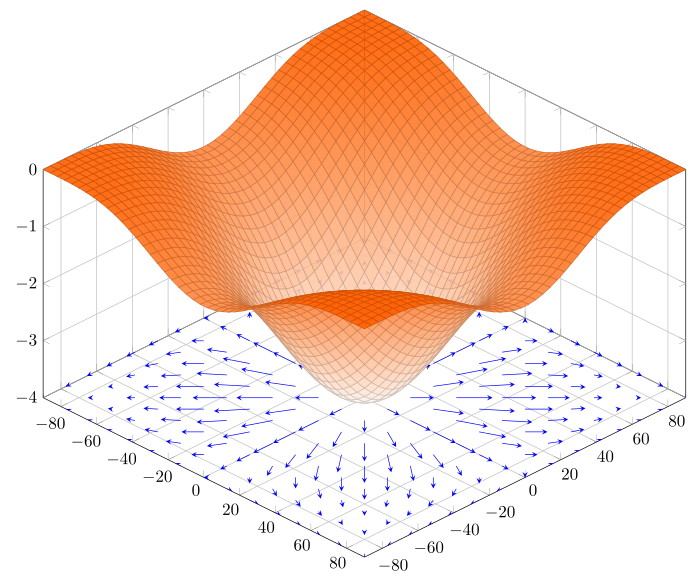
\includegraphics[scale=.3]{pics/gradient-cos.png}
\end{minipage}
\begin{alertblock}{Important geometric interpretation of the gradient}
	The gradient gives the direction of the steepest local increase of $f$.
\end{alertblock}

%	\begin{itemize}
%		%\item Generalization of derivatives in multidimensions.
%		%\item It is a vector representing the slope.
%		\item The direction of the gradient points to the gratest rate of increase of the function. 
%		%\item Its magnitude is the slope of the graph in its direction.
%	\end{itemize}
\end{frame}


\begin{frame}{Error minimization}
	\begin{itemize}
		\item Training statistical models always reduces to solving an optimization problem $${\rm minimize}_{\mathbf w}\;E(\mathbf w),\qquad\qquad \mathbf w^*:=\arg\min_{\mathbf w}\;E(\mathbf w).$$
%		\item Equivalently, we are interested in finding $w^*=\arg\min_w\;E(w)$.
		\item Standard approach is gradient descent $\mathbf w^{t+1}=\mathbf w^t-\eta\nabla E(\mathbf w^t)$, where $\eta\in (0,1]$ is the step size (aka \alert{learning rate}) with $w^0$ some initial point.\\[5mm]
		\item For the least squares, ${\rm minimize}\;E(\mathbf w)=\tfrac12\sum_{n=1}^N(\mathbf x_n^\top \mathbf w-t_n)^2$ we have $$\nabla E(\mathbf w)=\sum_{n=1}^N\mathbf x_n(\mathbf x_n^\top \mathbf w-t_n).$$
%		\item We choose an initial point $w^0$, and perform the following iterations $$w^{t+1}=w^t-\eta\nabla E(w^{t}).$$
	\end{itemize}
\end{frame}

\begin{frame}{Gradient descent derivation}
	\begin{itemize}
		\item Suppose we are at $\mathbf w$ and we want to pick a direction $\mathbf u$ such that $E(\mathbf w+\eta \mathbf u)$ is smaller than $E(\mathbf w)$ for a step size $\eta$, $\|\mathbf u\|=1$.
		\item The first-order Taylor series approximation of $E(\mathbf w+\eta \mathbf u)$ around $\mathbf w$ is: $$E(\mathbf w+\eta \mathbf u)\;=\;E(\mathbf w)+\eta\nabla E(\mathbf w)^\top \mathbf u +o(\eta)\;\approx\; E(\mathbf w)+\eta\nabla E(\mathbf w)^\top \mathbf u.$$
		\item Direction $u$ should have a negative inner product with $\nabla E(\mathbf w)$, e.g. $-\tfrac{\nabla E(\mathbf w)}{\|\nabla E(\mathbf w)\|}$. 
		\item This approximation gets better as $\eta$ gets smaller. 
	\end{itemize}
	\begin{exampleblock}{How do we choose the step size in GD? \;\;\;\;\;\;\;$\mathbf w^{t+1}=\mathbf w^t-\eta\nabla E(\mathbf w^t)$}
	\begin{itemize}
		\item Simple strategy: start with a big $\eta$ and progressively make it smaller by e.g. halving it until the function decreases.
		\item The sequence of step sizes is referred to as \alert{learning rate schedule}. 
	\end{itemize}
	\end{exampleblock}
\end{frame}

%\begin{frame}{How do we choose the step size?}
%	\begin{itemize}
%		\item The step size is referres as learning rate in machine learning.
%		%\item It should be in the interval $(0,1]$.
%		\item The sequence of step sizes is referred to as learning rate schedule. 
%		\item Simple strategy: start with a big $\eta$ and progressively make it smaller by e.g. halving it until the function decreases.
%		\item There are more formal ways of choosing the step size. But in practice, they are not used for computational reasons. 
%	\end{itemize}
%\end{frame}

\begin{frame}{When did the GD converge?}
	\begin{itemize}
		\item The vector $\mathbf w$ is a fixed point if $\nabla E(\mathbf w)=\mathbf 0$.\\[3mm]
		\item This is never possible in practice. So we stop iterations if gradient is smaller than a threshold, $\|\nabla E(\mathbf w)\|<\tau$. \\[3mm]
		\item If the function is convex then we have reached a global minimum.\\[3mm]
		\item If the function is not convex, what did we obtain?\\[3mm]
		\item Probably a local minimum or a saddle point. 
	\end{itemize}
\end{frame}

%\begin{frame}{Stochastic gradient descent}
%	\begin{itemize}
%		\item Any iteration of a gradient descent method requires that we sum over the entire dataset to compute the gradient.
%		\item SGD idea: at each iteration, sub-sample a small amount of data (even just 1 point can work) and use that to estimate the gradient.
%		\item Each update is noisy, but very fast!
%		\item This is the basis of optimizing ML algorithms with huge datasets (e.g. deep learning).
%		\item Computing gradients using the full dataset is called batch learning, using subsets of data is called mini-batch learning.
%	\end{itemize}
%\end{frame}


\begin{frame}{Stochastic Gradient Descent}
In most cases, we minimize an average over data points: $$E(\mathbf w)=\tfrac1N\sum_{i=1}^N L(t_n,y(\mathbf x_n,\mathbf w)),\qquad \nabla E(\mathbf w)\;=\;\tfrac1N\sum_{n=1}^n \nabla L(t_n,y(\mathbf x_n,\mathbf w)),$$
which is hard to compute when $N$ is very large.

At each iteration, use a sub-sample of data  to estimate the gradient
$$
\mathbf w^{t+1}=\mathbf w^t-\eta\frac{1}{|S|}\sum_{n\in S}\nabla L(t_n,y(\mathbf x_n,\mathbf w)).
$$
{\small (Here $|S|$ denotes the number of elements in the set $S$. Standard SGD has $|S|=1$)}\\[3mm]
ML terminology: Computing gradients using the full dataset is called \alert{batch learning}, using subsets of data is called \alert{mini-batch learning}.
\end{frame}




\section{Introducing neural networks}


\begin{frame}{A Simpler Neuron}
For neural nets, we use a simple model for neuron, or \textbf{unit}:

    \begin{center}
      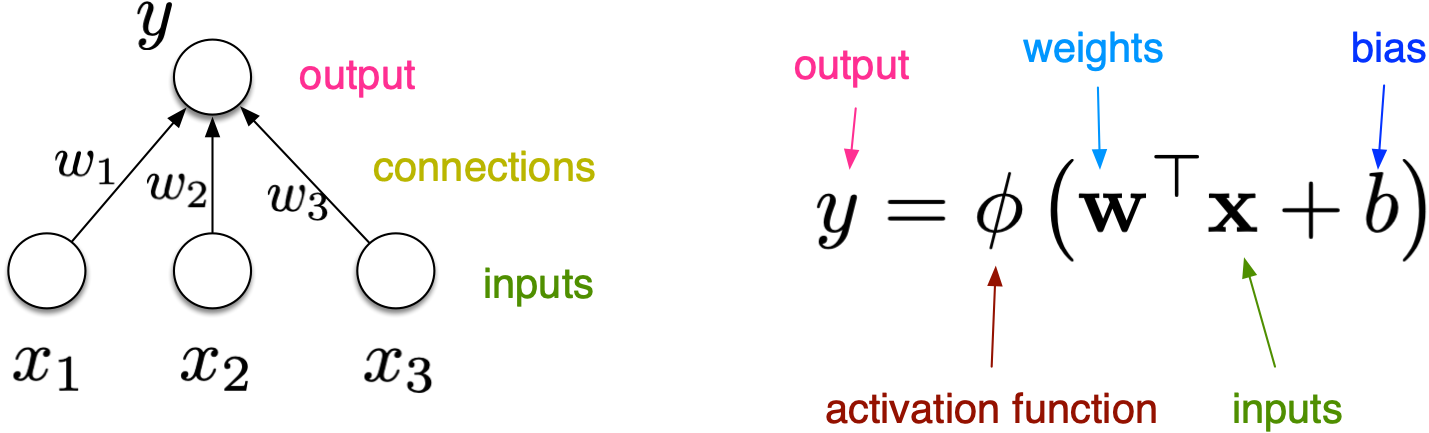
\includegraphics[width=0.8 \textwidth]{pics/neuron2}
    \end{center}
\pause
  \begin{itemize}

  \item By throwing together lots of these simple neuron-like processing units, we can do some powerful computations!
  \end{itemize}
\end{frame}



\begin{frame}{A Feed-Forward Neural Network}
\vspace{5mm}
  \begin{columns}
    \begin{column}{0.45 \linewidth}
      \begin{itemize}
      \item A \high{directed acyclic graph}
      \item Units are grouped into \high{layers}
      \end{itemize}
    \end{column}
    \begin{column}{0.65 \linewidth}
      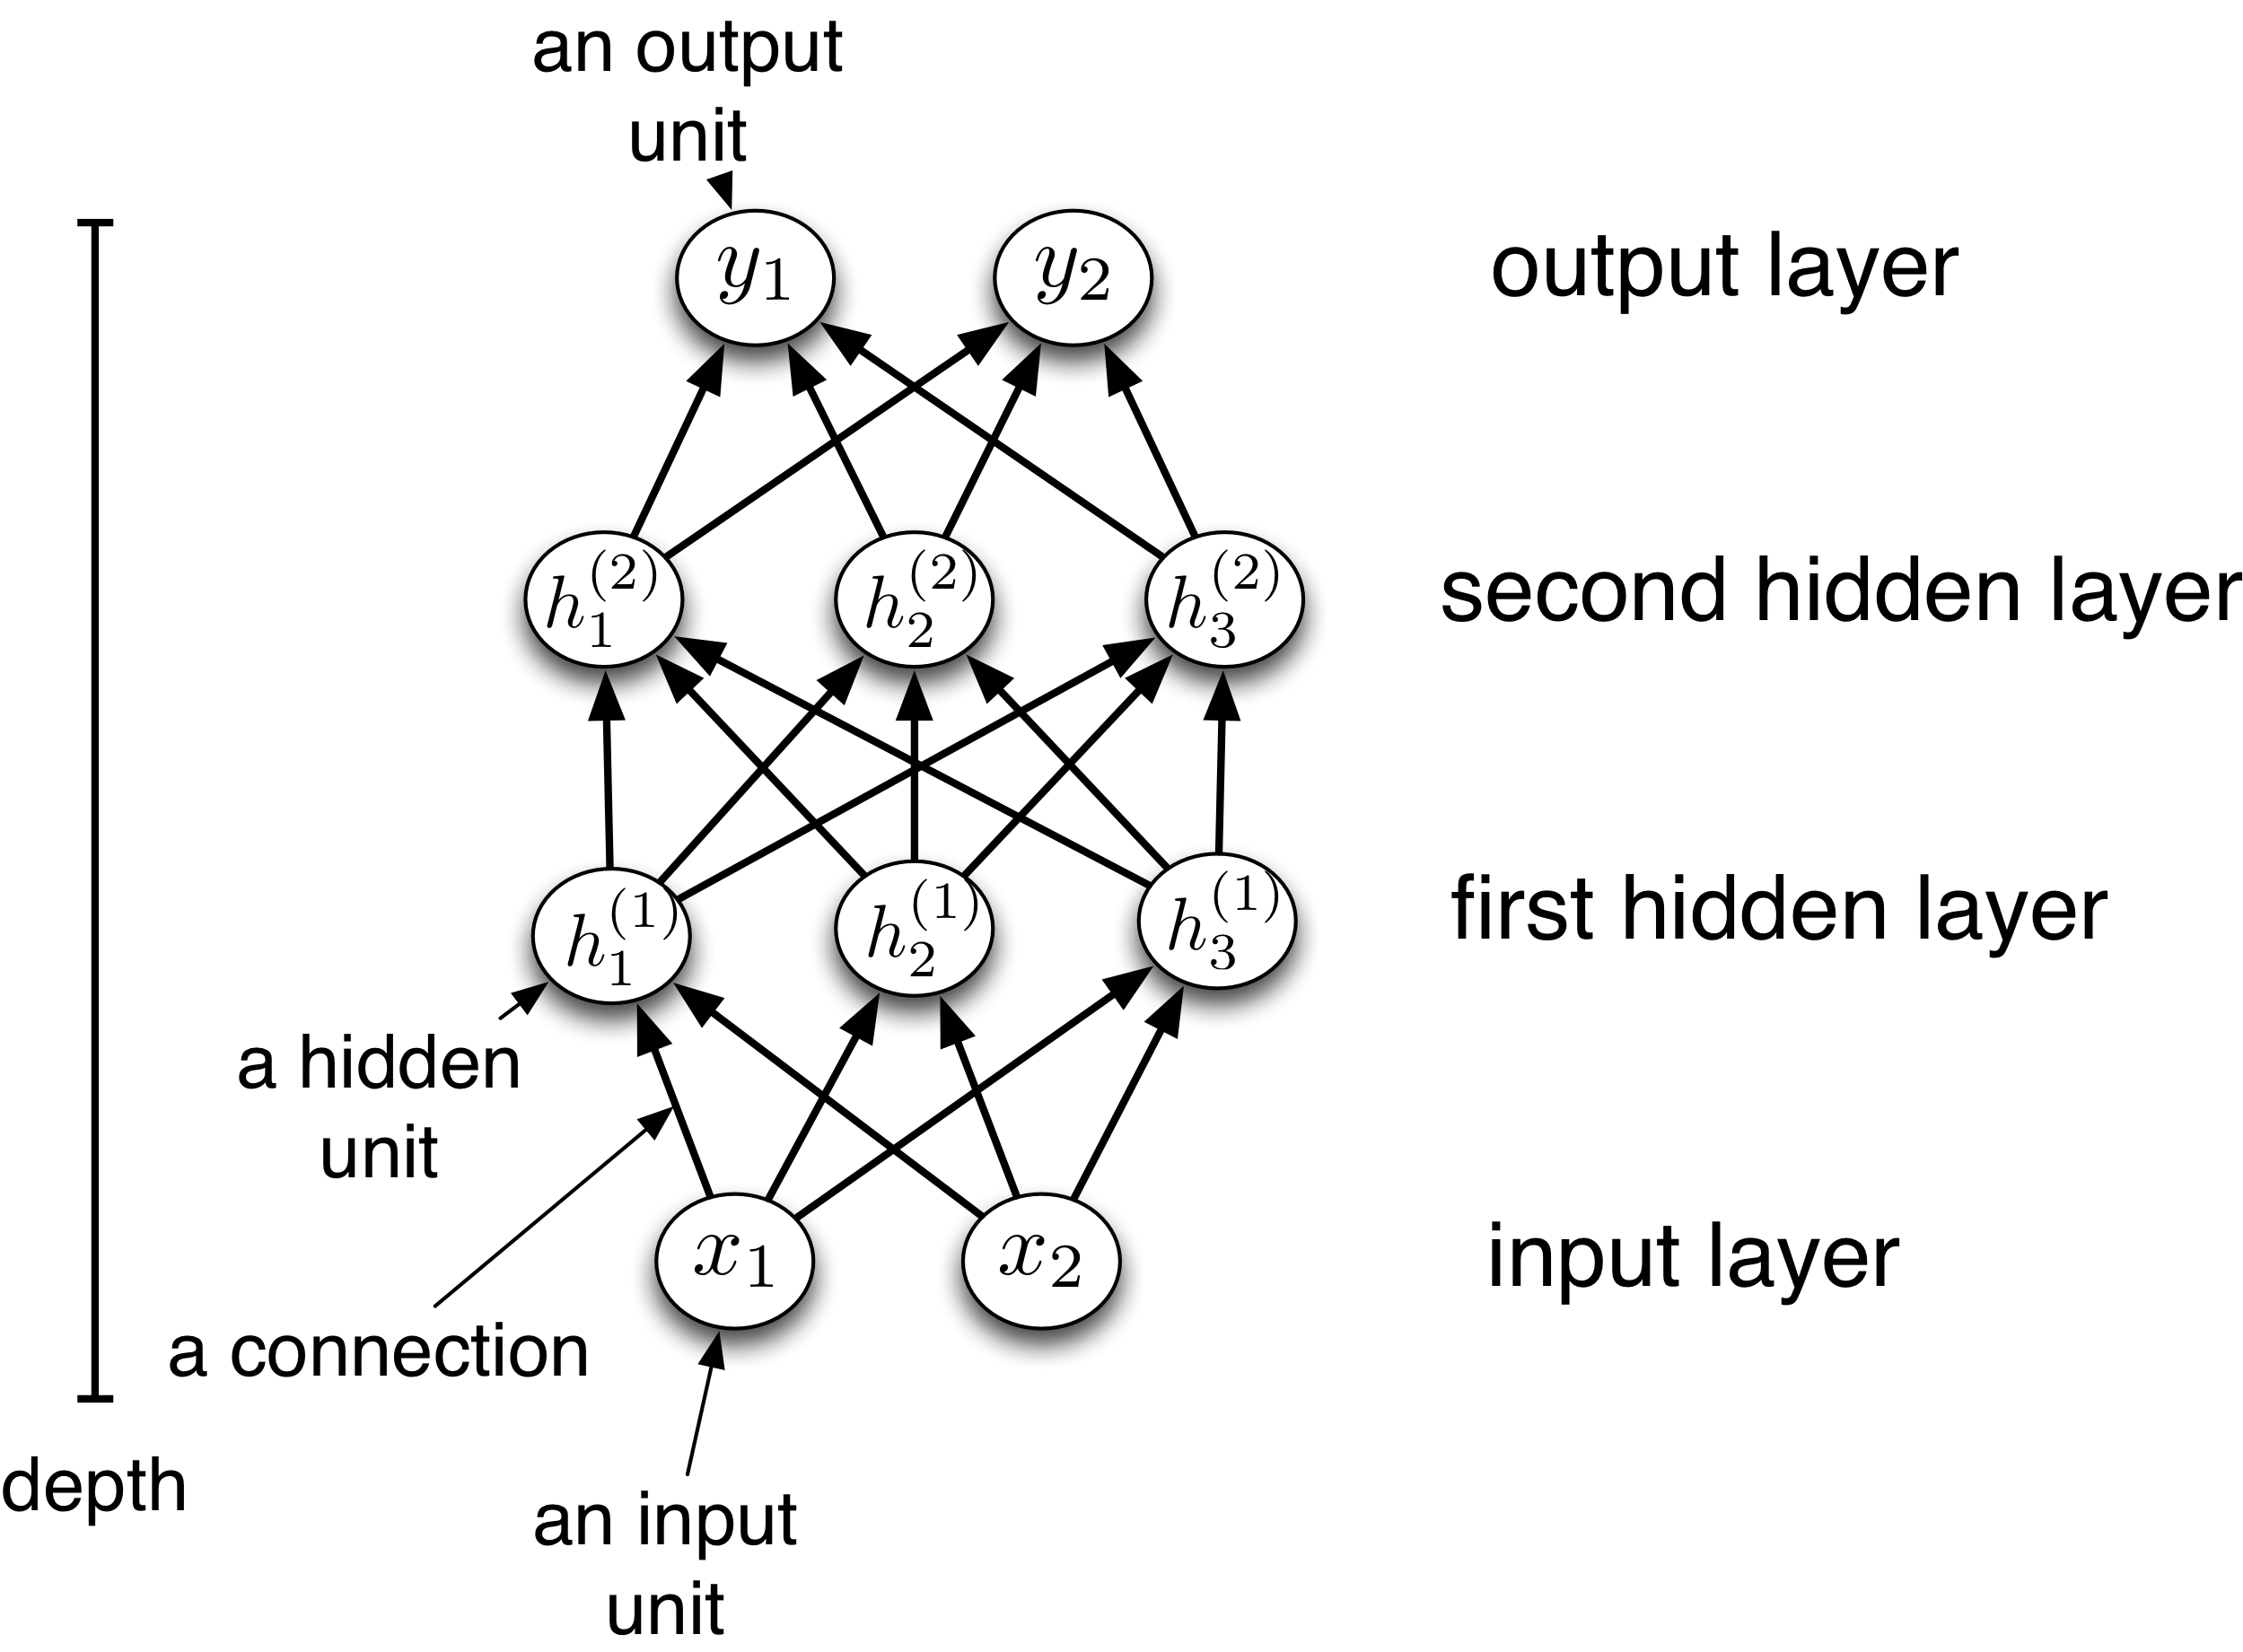
\includegraphics[width=\linewidth]{pics/mlp.png}
    \end{column}
  \end{columns}
\end{frame}

\begin{frame}{Multilayer Perceptrons}
\begin{itemize}
\item A multi-layer network consists of fully connected layers.
\item In a fully connected layer, all input units are connected to 
all output units.
%\item Each hidden layer $i$ connects $N_{i-1}$ input units to $N_{i}$ output
%  units. Weight matrix is $N_i$ x $N_{i-1}$.
\pause
\item The outputs are a function of the input units:
        \[ \predictions = \function(\inputVec) = \activationFunction \left( \weightMat \inputVec + \biases \right) \]
        $\activationFunction:\R\to \R$ is applied \alert{component-wise}.
\end{itemize}
\vspace{-4mm}
\begin{center}
  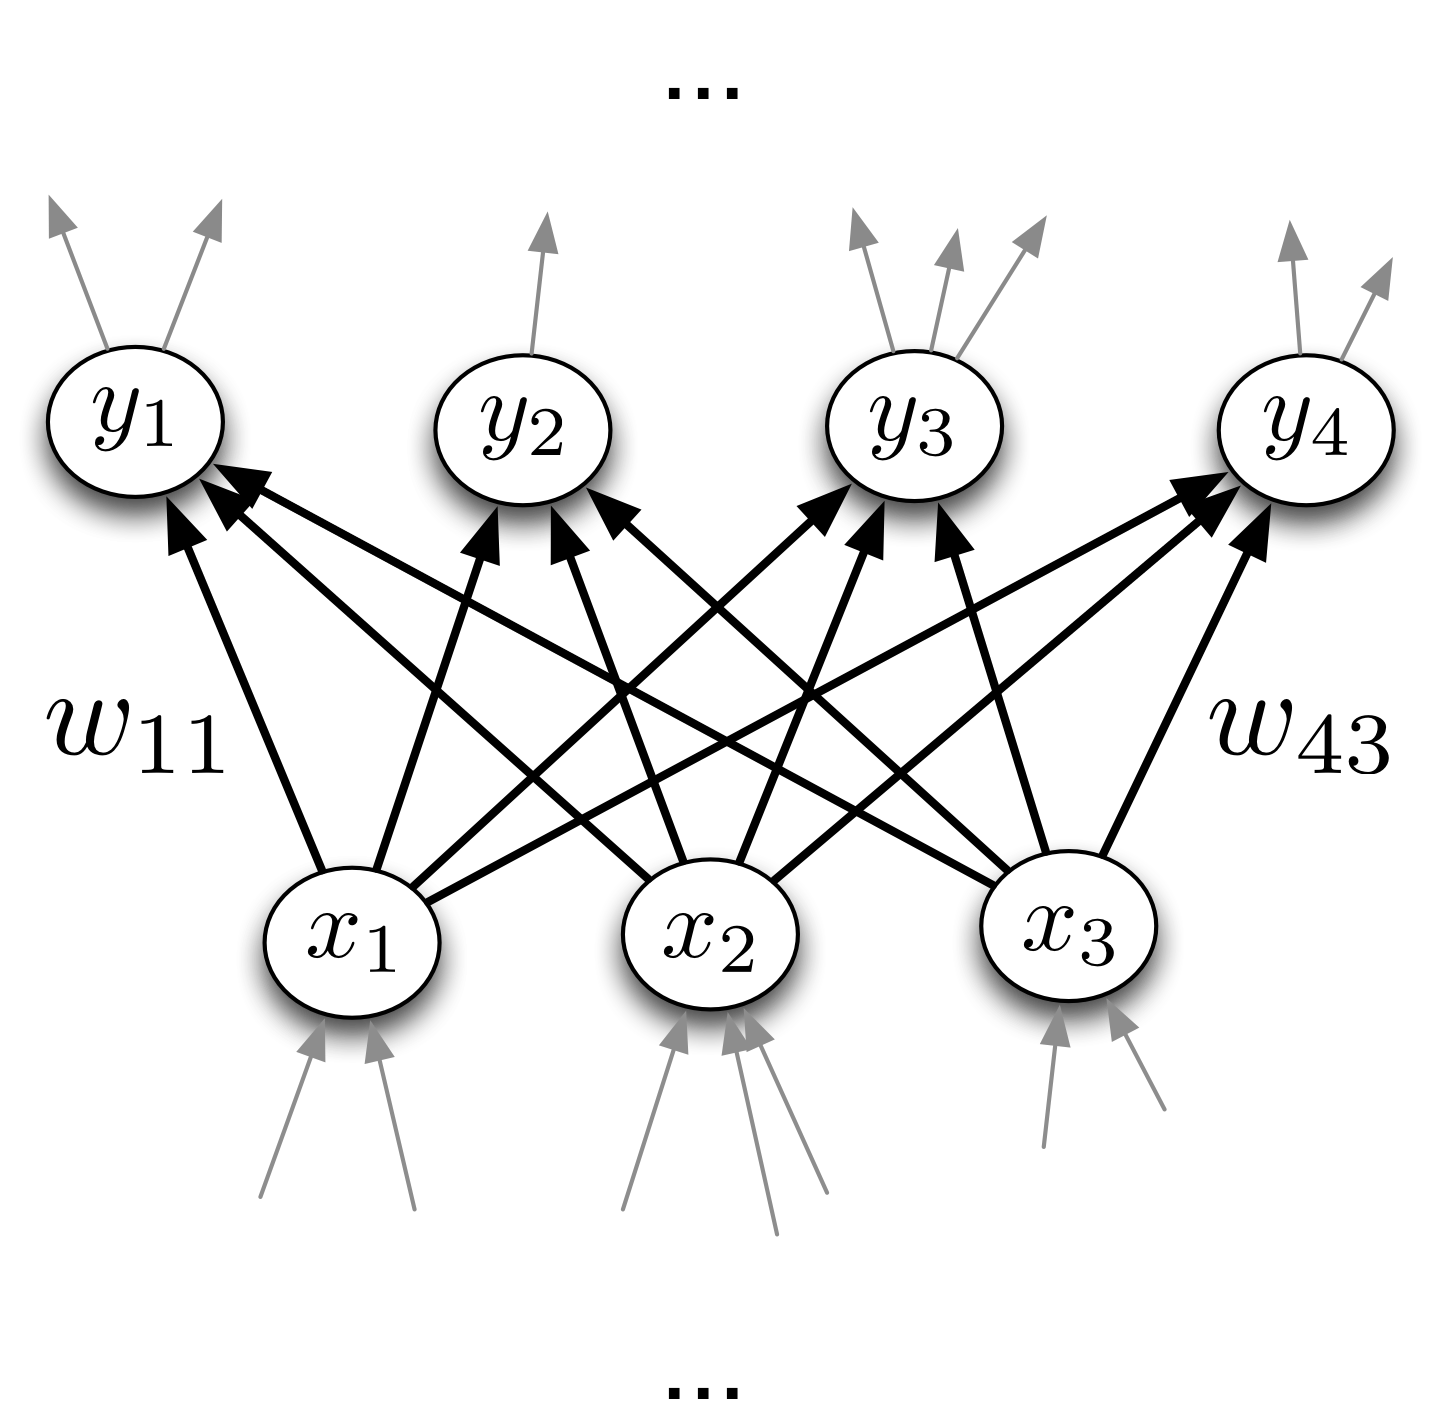
\includegraphics[width=0.3\linewidth]{pics/fc_layer.png}
\end{center}
\end{frame}


\begin{frame}{Some Activation Functions}
  \begin{columns}
    \begin{column}{0.25 \linewidth}
      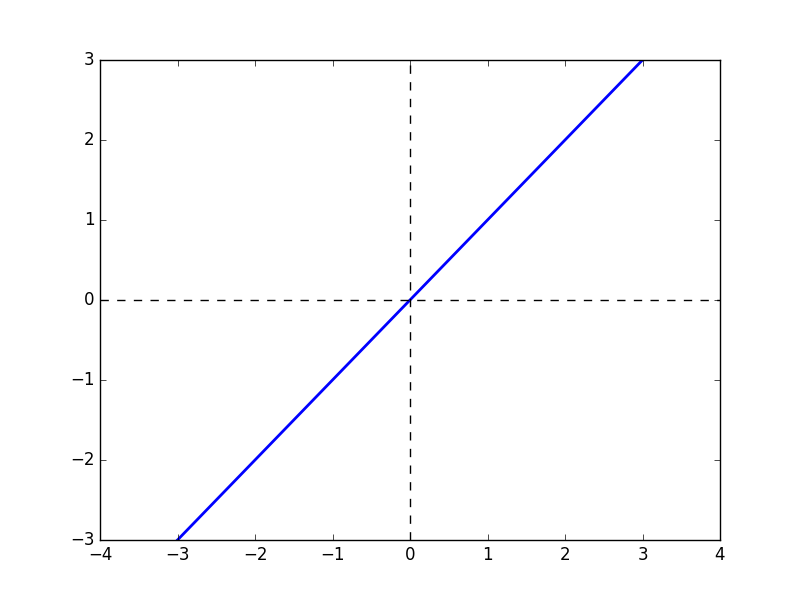
\includegraphics[width=\linewidth]{pics/act_lin.png}
      \begin{center}
        {\bf Identity}
      \end{center}
      \[ \phi(z) = z \]
    \end{column}

    \begin{column}{0.4 \linewidth}
    \centering
      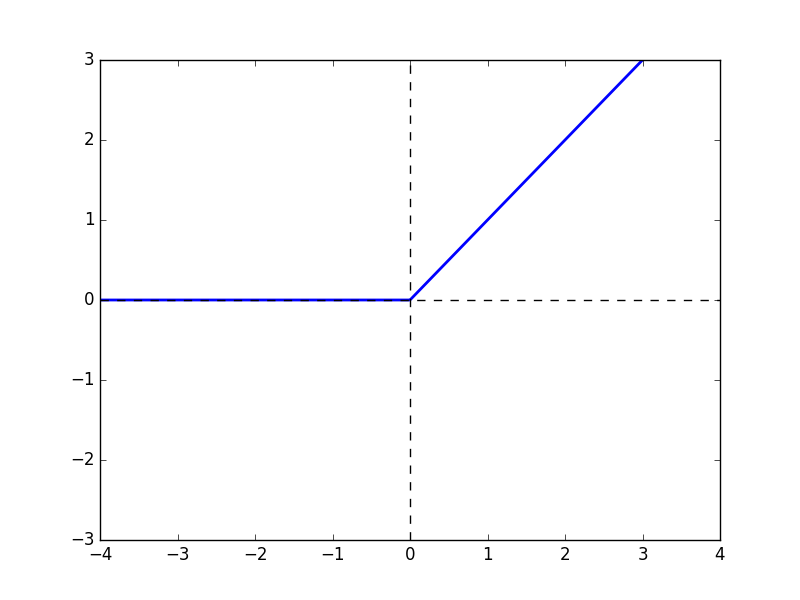
\includegraphics[width=0.8\linewidth]{pics/act_relu.png}
      \begin{center}
        {\bf Rectified Linear Unit} \\
        {\bf (ReLU)}
      \end{center}
      \[ \phi(z) = \max(0, z) \]
    \end{column}

    \begin{column}{0.25 \linewidth}
      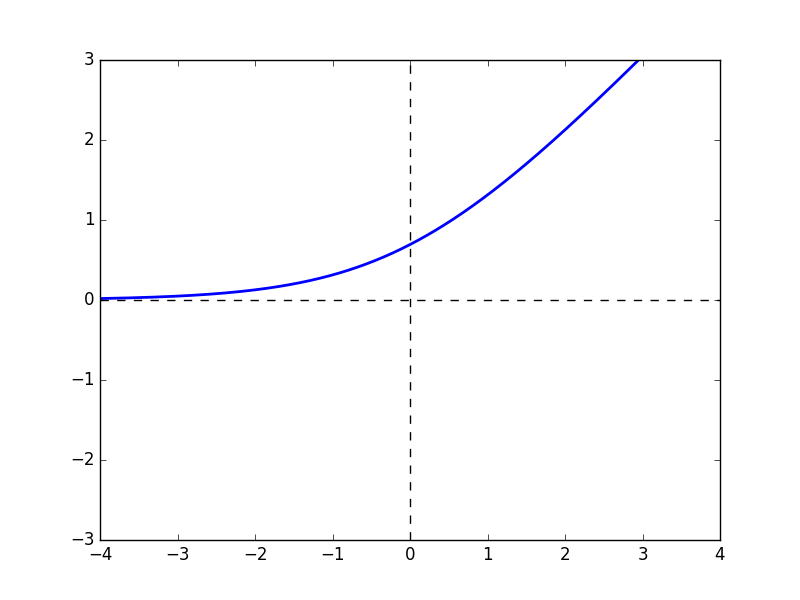
\includegraphics[width=\linewidth]{pics/act_soft_relu.png}
      \begin{center}
        {\bf Soft ReLU}
      \end{center}
      \[ \phi(z) = \log 1 + e^z \]
    \end{column}
  \end{columns}
\end{frame}

\begin{frame}{More Activation Functions}
  \begin{columns}
    \begin{column}{0.3 \linewidth}
      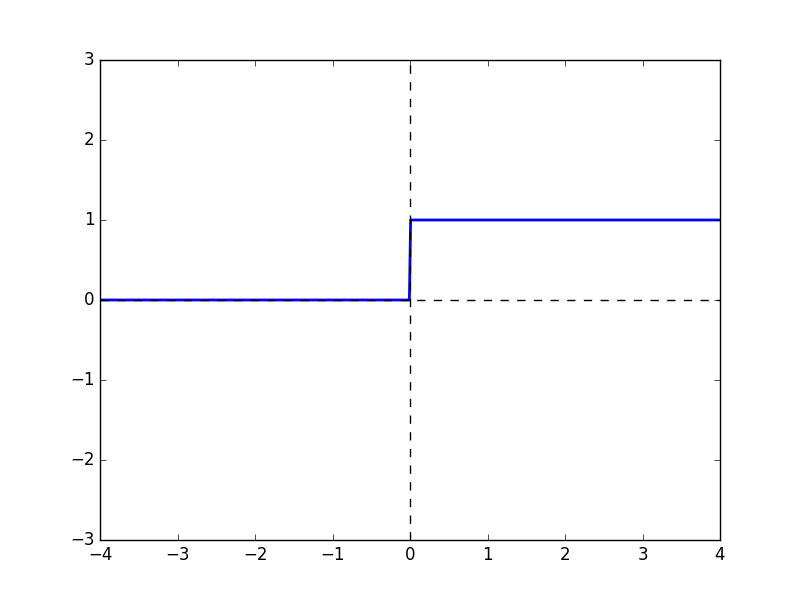
\includegraphics[width=\linewidth]{pics/act_threshold.png}
      \begin{center}
        {\bf Hard Threshold}
      \end{center}
      \[ \phi(z) = \left\{ \begin{array}{ll} 1 & \textrm{if } z > 0 \\ 0 & \textrm{if } z \leq 0 \end{array} \right. \]
    \end{column}

    \begin{column}{0.3 \linewidth}
      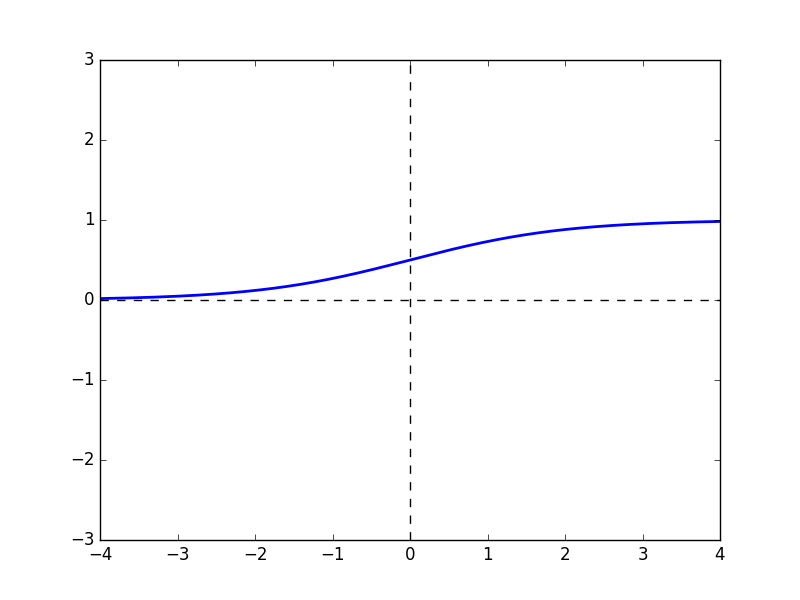
\includegraphics[width=\linewidth]{pics/act_logistic.png}
      \begin{center}
        {\bf Logistic}
      \end{center}
      \[ \phi(z) = \frac{1}{1+e^{-z}} \]
    \end{column}

    \begin{column}{0.3 \linewidth}
      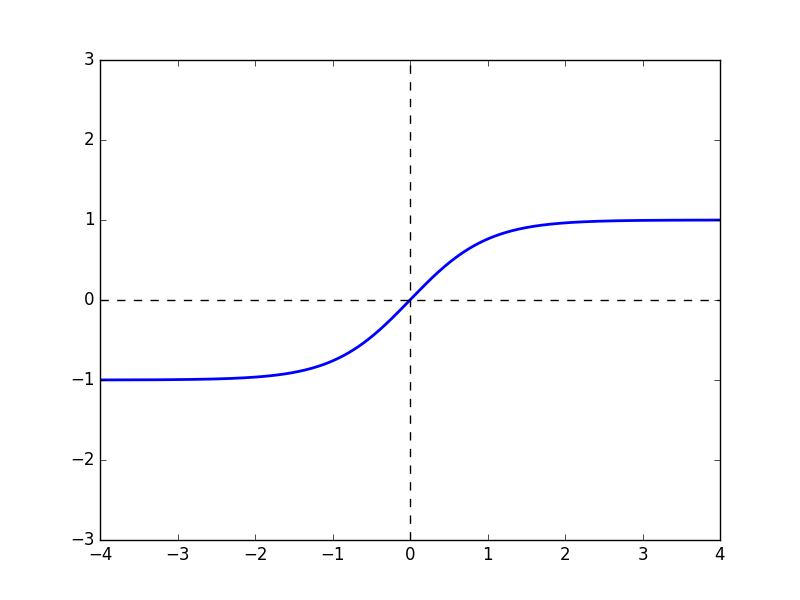
\includegraphics[width=\linewidth]{pics/act_tanh.png}
      \begin{center}
        {\bf Hyperbolic Tangent} \\
        {\bf (tanh)}
      \end{center}
      \[ \phi(z) = \frac{e^{z} - e^{-z}}{e^{z} + e^{-z}} \]
    \end{column}
  \end{columns}
\end{frame}


\begin{frame}{Computation in Each Layer}
\medskip 

\begin{columns}
\begin{column}{0.75\linewidth}
%\centering

Each layer computes a function.
\begin{align*}
          \hiddensL{1} &= \functionL{1}(\inputVec) = \phi(\weightMat^{(1)} \inputVec + \biases^{(1)}) \\
          \hiddensL{2} &= \functionL{2}(\hiddensL{1}) = \phi(\weightMat^{(2)} \hiddensL{1} + \biases^{(2)})\\
                       & \hspace{0.5em} \vdots \\
          \predictions &= \functionL{\numLayers}(\hiddensL{\numLayers-1})
\end{align*}
\bigskip
\pause 
The network computes a composition of functions.\\[-7mm]
        \[ \predictions = \functionL{\numLayers} \circ \cdots \circ \functionL{1}(\inputVec). \]

\pause{
The last layer depends on the task.
\begin{itemize}
\item Regression: \quad $\predictions = \functionL{\numLayers}(\hiddensL{\numLayers-1}) = (\weights^{(L)})^{\top} \hiddensL{\numLayers-1} + b^{(L)}$
\item Classification:  $\predictions = \functionL{\numLayers}(\hiddensL{\numLayers-1}) = \alert{\sigma\big(}(\weights^{(L)})^{\top} \hiddensL{\numLayers-1} + b^{(L)}\alert{\big)}$
\end{itemize}
}
\bigskip

\end{column}
\begin{column}{0.35\linewidth}
    \centering
      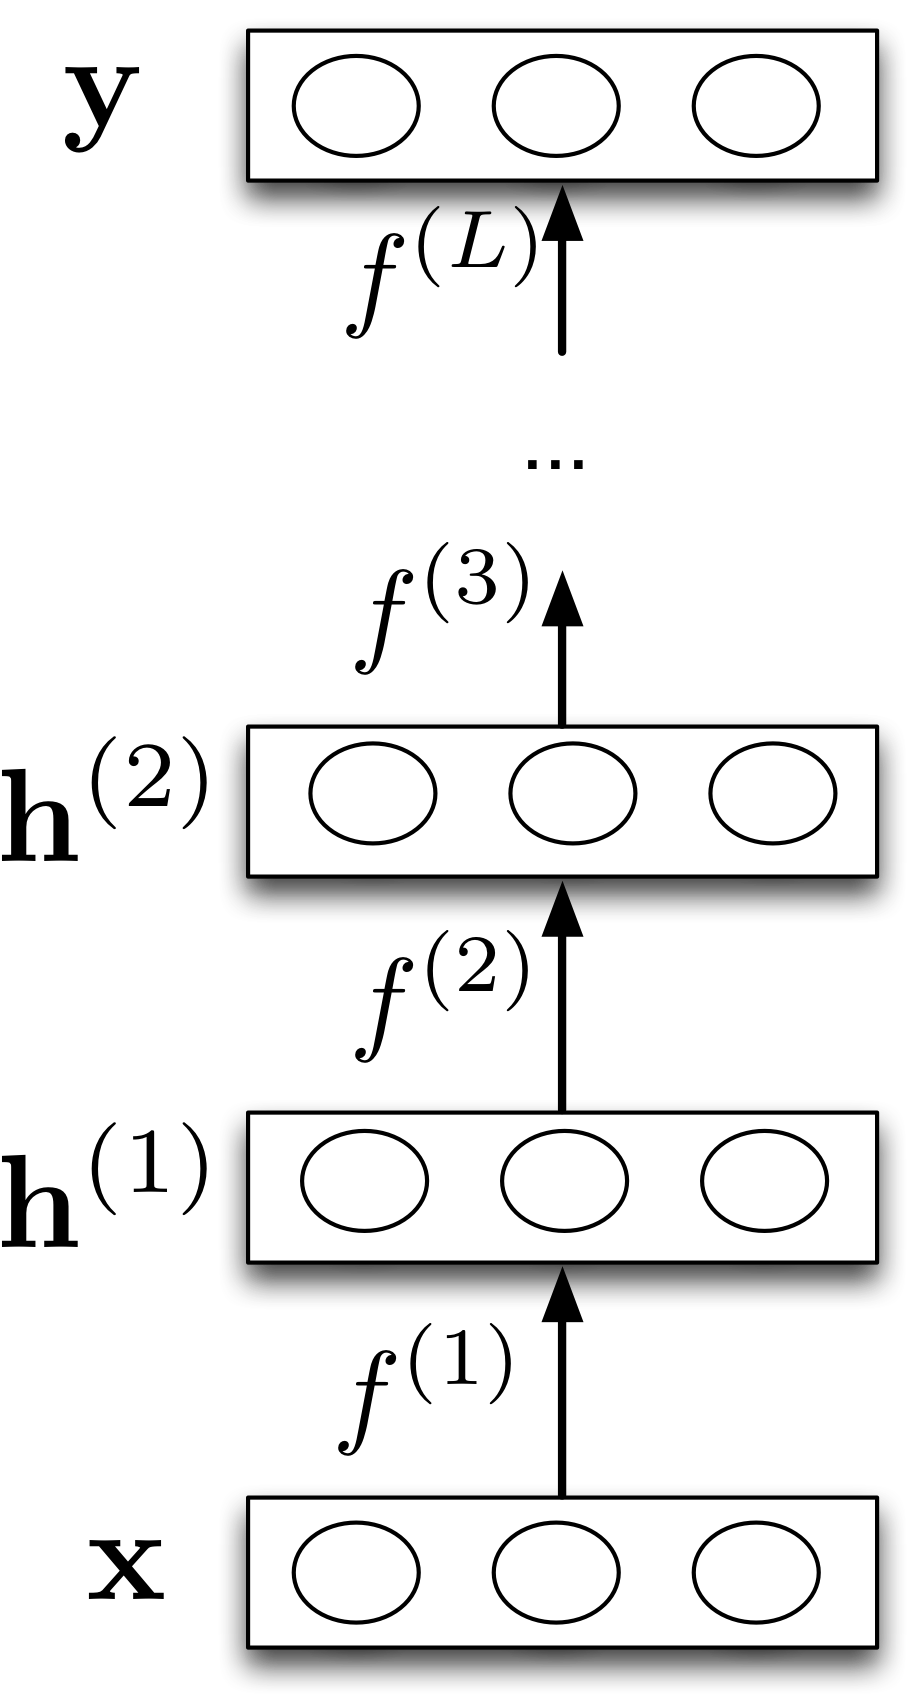
\includegraphics[width=.7\linewidth]{pics/layer_functions.png}
\end{column}
\end{columns}
\end{frame}


\begin{frame}{Expressive Power of Linear Networks}
  \begin{itemize}
  \setlength\itemsep{1em}
  \item Consider a linear layer: the activation function was the identity. The layer just computes an affine transformation of the input.
  \item Any sequence of linear layers is equivalent to a single linear layer.
    \[ \predictions = \underbrace{\weightMatL{3} \weightMatL{2} \weightMatL{1}}_{\triangleq \weightMat^\prime} \inputVec \]
\item Deep linear networks can only represent linear functions 
--- no more expressive than linear regression.
  \end{itemize}
\end{frame}


\begin{frame}{Expressive Power of Non-linear Networks}
  \begin{itemize}
  \setlength\itemsep{1em}
    \item Multi-layer feed-forward neural networks  with non-linear activation functions
    \item \textbf{Universal Function Approximators}:  They can approximate any function arbitrarily well.
      %, \\
   % i.e., for any $f : \mathcal{X} \to \mathcal{T}$ there is a sequence $f_i \in \mathcal{H}$ with $f_i \to f$.
    \item True for various activation functions  (e.g. thresholds, logistic, ReLU, etc.)
  \end{itemize}
%      \begin{figure}
%      \centering
%      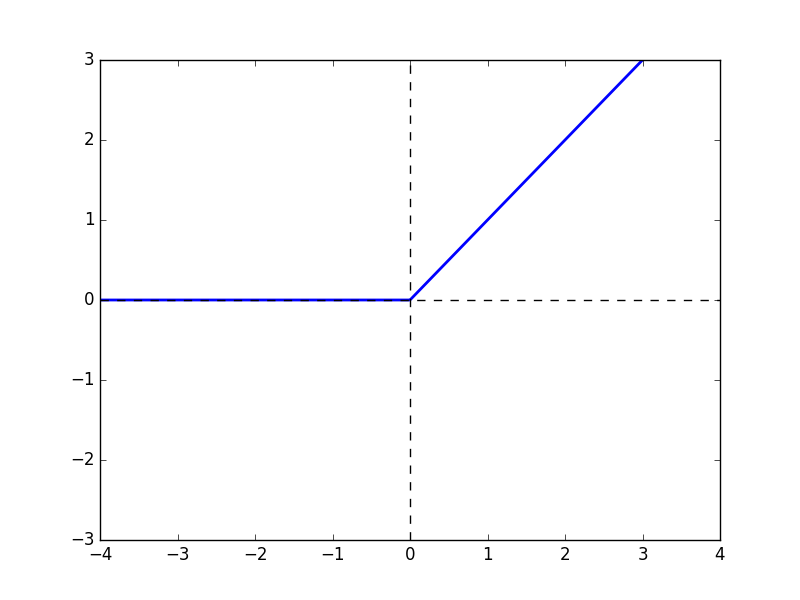
\includegraphics[width=0.4\linewidth]{pics/act_relu.png}
%      \end{figure}
\end{frame}




\begin{frame}{Expressivity of the Logistic Activation Function}
  \begin{itemize}
    \item What about the logistic activation function?
    \item Approximate a hard threshold by scaling up $w$ and $b$.
      \begin{columns}
        \begin{column}{0.4 \textwidth}
          \begin{center}
            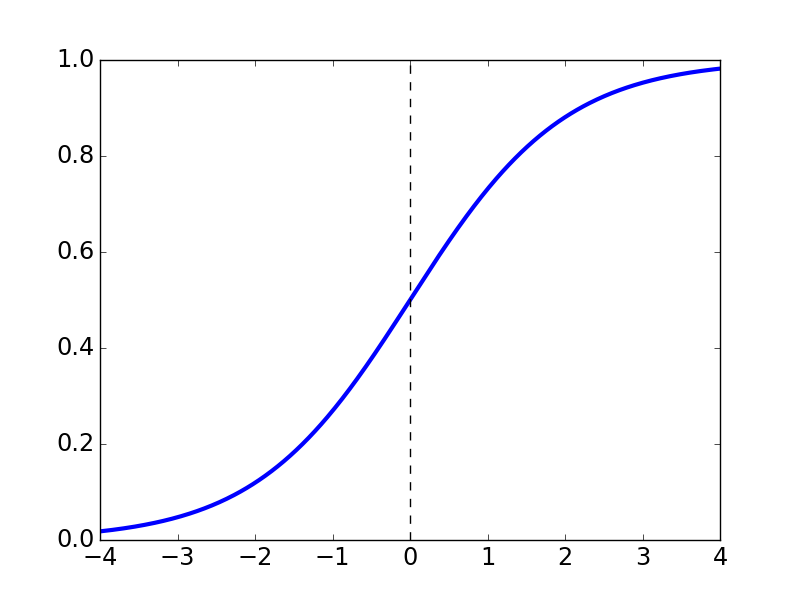
\includegraphics[width=0.8 \textwidth]{pics/scaling_1.png}
          \end{center}
          \[ y = \sigma(x) \]
        \end{column}
        \begin{column}{0.4 \textwidth}
          \begin{center}
            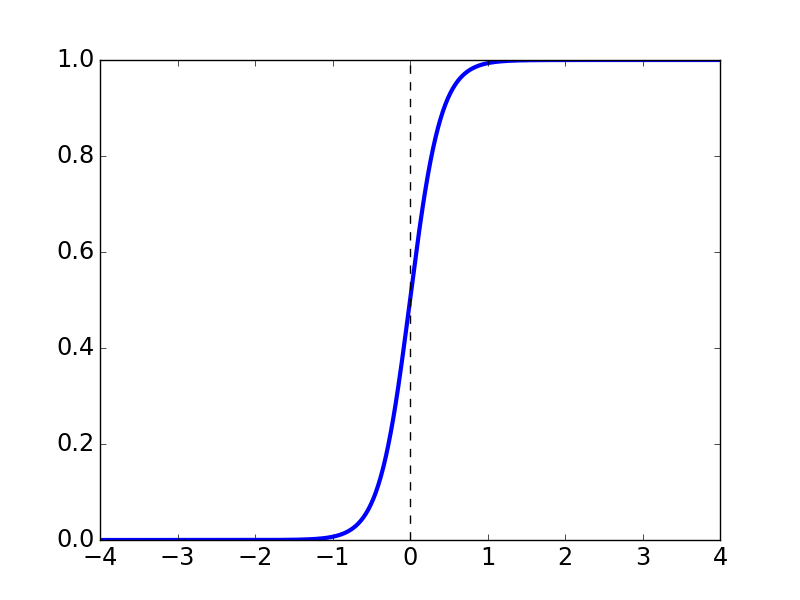
\includegraphics[width=0.8 \textwidth]{pics/scaling_5.png}
          \end{center}
          \[ y = \sigma(5x) \]
        \end{column}
      \end{columns}

      \vspace{0.5em}
    \pause
    \item Logistic units are differentiable, so we can learn weights with gradient descent.
  \end{itemize}
\end{frame}


\begin{frame}{What is Expressivity Good For?}

\begin{itemize}

\item May need a very large network to represent a function.
\item Non-trivial to learn the weights that represent a function.
\item If you can learn any function, over-fitting is potentially a serious concern!
\bigskip

For the polynomial feature mappings, expressivity increases with the degree $M$, eventually allowing multiple perfect fits to the training data. This motivated $L^2$ regularization.
\begin{center}
    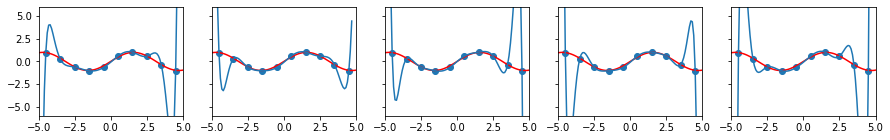
\includegraphics[width=0.8\textwidth]{pics/multiple_memorizations.png}
\end{center}
\bigskip

\item Do neural networks over-fit and how can we regularize them?
\end{itemize}
\end{frame}


\begin{frame}{Regularization and Over-fitting for Neural Networks}
	\begin{itemize}
    \item The topic of over-fitting (when \& how it happens, how to regularize, etc.) for neural networks is not well-understood, even by researchers!
    \begin{itemize}
      \item In principle, you can always apply $L^2$ regularization.
   %   \item You will learn more in CSC413.
    \end{itemize}
    \item A common approach is \high{early stopping}, or stopping training early, because over-fitting typically increases as training progresses.
		\begin{center}
			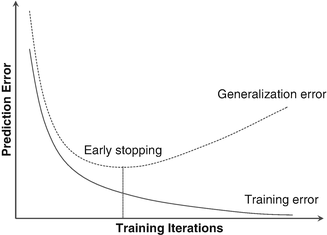
\includegraphics[width=0.4\textwidth]{pics/learning_curves.png}
		\end{center}
%\item Don't add an explicit $\mathcal{R}(\btheta)$ term to our cost.
\item \alert{Benign overfitting} is a heavily studied phenomenon.
	\end{itemize}
\end{frame}



\section{Backpropagation}
%\begin{frame}
%  \tableofcontents[sectionstyle=show/shaded,subsectionstyle=show/shaded/hide]
%\end{frame}

\begin{frame}{Learning Weights in a Neural Network}

\begin{itemize}
\item Goal is to learn weights in a multi-layer neural network 
using gradient descent.
\medskip

\item Weight space for a multi-layer neural net: one set of weights for each unit in every layer of the network
\medskip

\item Define a loss $\loss(\target,y)=\loss(\target,y(x,\weights))$ and compute the gradient of the cost $$E(\weights)\;=\;\tfrac1N\sum_{n=1}^N \loss(\target_n,y(x_n,\weights)),$$
which is the average loss over all the training examples.
\medskip

\item How we can calculate $\nabla E ( \weights)$ efficiently?
\end{itemize}
\end{frame}


\begin{frame}{Example: Two-Layer Neural Network}
\begin{figure}
\begin{tikzpicture}
\tikzstyle{nodestyle}=[draw, circle, font=\bfseries\large]
    \node[nodestyle] (1t1) at (0,6) {$1$};
    \node[nodestyle] (x1) at (0,4.3) {$x_1$};
    \node[nodestyle] (x2) at (0,1.7) {$x_2$};
    \node[nodestyle] (1b1) at (0,0) {$1$};
    \node[nodestyle] (h1) at (3,4.3) {$h_1$};
    \node[nodestyle] (h2) at (3,1.7) {$h_2$};
    \node[nodestyle] (2t1) at (3,6) {$1$};
    \node[nodestyle] (y1) at (6,4.3) {$y_1$};
    \node[nodestyle] (y2) at (6,1.7) {$y_2$} ;
    \node[nodestyle] (2b1) at (3,0) {$1$};
    \draw [-{Latex[length=3mm]}] (x1) -- (h1) node [near start, above] {$w^{(1)}_{11}$};
    \draw [-{Latex[length=3mm]}] (x1) -- (h2) node [near start, above] {$w^{(1)}_{12}$};
    \draw [-{Latex[length=3mm]}] (1t1) -- (h1) node [near start, above] {$w^{(1)}_{01}$};
    \draw [-{Latex[length=3mm]}] (x2) -- (h1) node [near start, below] {$w^{(1)}_{21}$};
    \draw [-{Latex[length=3mm]}] (x2) -- (h2) node [near start, below] {$w^{(1)}_{22}$};
    \draw [-{Latex[length=3mm]}] (1b1) -- (h2) node [near start, below] {$w^{(1)}_{02}$};   
    \draw [-{Latex[length=3mm]}] (h1) -- (y1) node [near start, above] {$w^{(2)}_{11}$};
    \draw [-{Latex[length=3mm]}] (h1) -- (y2) node [near start, above] {$w^{(2)}_{21}$};
    \draw [-{Latex[length=3mm]}] (2t1) -- (y1) node [near start, above] {$w^{(2)}_{01}$};
    \draw [-{Latex[length=3mm]}] (h2) -- (y1) node [near start, below] {$w^{(2)}_{12}$};
    \draw [-{Latex[length=3mm]}] (h2) -- (y2) node [near start, below] {$w^{(2)}_{22}$};
    \draw [-{Latex[length=3mm]}] (2b1) -- (y2) node [near start, below] {$w^{(2)}_{02}$};
\end{tikzpicture}
\caption{Two-Layer Neural Network}
\end{figure}
\end{frame}


\begin{frame}[t]{Computations for Two-Layer Neural Network}
A neural network computes a composition of functions.
\begin{minipage}{6cm}
{\small 
	\begin{tikzpicture}[scale=.7]
\tikzstyle{nodestyle}=[draw, circle, font=\bfseries\small]
    \node[nodestyle] (1t1) at (0,6) {$1$};
    \node[nodestyle] (x1) at (0,4.3) {$x_1$};
    \node[nodestyle] (x2) at (0,1.7) {$x_2$};
    \node[nodestyle] (1b1) at (0,0) {$1$};
    \node[nodestyle] (h1) at (3,4.3) {$h_1$};
    \node[nodestyle] (h2) at (3,1.7) {$h_2$};
    \node[nodestyle] (2t1) at (3,6) {$1$};
    \node[nodestyle] (y1) at (6,4.3) {$y_1$};
    \node[nodestyle] (y2) at (6,1.7) {$y_2$} ;
    \node[nodestyle] (2b1) at (3,0) {$1$};
    \draw [-{Latex[length=2mm]}] (x1) -- (h1) node [near start, above] {$w^{(1)}_{11}$};
    \draw [-{Latex[length=2mm]}] (x1) -- (h2) node [near start, above] {$w^{(1)}_{12}$};
    \draw [-{Latex[length=2mm]}] (1t1) -- (h1) node [near start, above] {$w^{(1)}_{01}$};
    \draw [-{Latex[length=2mm]}] (x2) -- (h1) node [near start, below] {$w^{(1)}_{21}$};
    \draw [-{Latex[length=2mm]}] (x2) -- (h2) node [near start, below] {$w^{(1)}_{22}$};
    \draw [-{Latex[length=2mm]}] (1b1) -- (h2) node [near start, below] {$w^{(1)}_{02}$};   
    \draw [-{Latex[length=2mm]}] (h1) -- (y1) node [near start, above] {$w^{(2)}_{11}$};
    \draw [-{Latex[length=2mm]}] (h1) -- (y2) node [near start, above] {$w^{(2)}_{21}$};
    \draw [-{Latex[length=2mm]}] (2t1) -- (y1) node [near start, above] {$w^{(2)}_{01}$};
    \draw [-{Latex[length=2mm]}] (h2) -- (y1) node [near start, below] {$w^{(2)}_{12}$};
    \draw [-{Latex[length=2mm]}] (h2) -- (y2) node [near start, below] {$w^{(2)}_{22}$};
    \draw [-{Latex[length=2mm]}] (2b1) -- (y2) node [near start, below] {$w^{(2)}_{02}$};
\end{tikzpicture}}
\end{minipage}
\begin{minipage}{7cm}
\begin{align*}
\large
& z^{(1)}_1 = w^{(1)}_{01} \cdot 1 + w^{(1)}_{11} \cdot  x_1 + w^{(1)}_{21} \cdot  x_2\\
& \qquad h_1 = \sigma (z_1) \\
& z^{(2)}_1 = w^{(2)}_{01} \cdot  1 + w^{(2)}_{11} \cdot  h_1 + w^{(2)}_{21} \cdot  h_2 \\
& \qquad y_1 = z_1 \\
& z^{(1)}_2 = \\
& \qquad h_2 = \\
& z^{(2)}_2 = \\
& \qquad y_2 = \\
& \loss = \frac{1}{2} \left( (y_1 - t_1)^2 + (y_2 - t_2)^2 \right)
\end{align*}	
\end{minipage}
\end{frame}


\begin{frame}{Simplified Example: Logistic Least Squares}
\begin{minipage}{0.3\textwidth}
\begin{align*}
\Large
    \intermediate &= \weightUni \inputUni + \bias \\[3mm]
    \prediction &= \sigmoid(\intermediate) \\[3mm]
    \loss &= \frac{1}{2} (\prediction - \target)^2 \\
\end{align*}
\end{minipage}\begin{minipage}{0.69\textwidth}
\begin{figure}
\begin{tikzpicture}
\tikzstyle{nodestyle}=[draw=none, font=\bfseries\huge]

    \node[nodestyle] (x) at (0,3) {$x$};
    \node[nodestyle] (b) at (0,2) {$b$};
    \node[nodestyle] (w) at (0,1) {$w$};
    \node[nodestyle] (z) at (2,2) {$z$};
    \node[nodestyle] (y) at (4,2) {$y$};
    \node[nodestyle] (t) at (4,3) {$t$} ;
    \node[nodestyle] (l) at (6,2) {$\loss$} ;

    \draw [-{Latex[length=3mm]}] (x) -- (z);
    \draw [-{Latex[length=3mm]}] (w) edge (z);
    \draw [-{Latex[length=3mm]}] (b) edge (z);
    \draw [-{Latex[length=3mm]}] (z) edge (y);
    \draw [-{Latex[length=3mm]}] (t) edge (l);
    \draw [-{Latex[length=3mm]}] (y) edge (l);
\end{tikzpicture}
\end{figure}
\end{minipage}
\alert{Computation Graph}:
\begin{itemize}
\item The nodes represent the inputs and computed quantities.
\item The edges represent which nodes are computed directly as a function of which other nodes.
\end{itemize}
\end{frame}


%\begin{frame}{Computation Graph}
%\begin{itemize}
%\item The nodes represent the inputs and computed quantities.
%\item The edges represent which nodes are computed directly as a function of which other nodes.
%\end{itemize}
%\begin{figure}
%\begin{tikzpicture}
%\tikzstyle{nodestyle}=[draw=none, font=\bfseries\huge]
%
%    \node[nodestyle] (x) at (0,3) {$x$};
%    \node[nodestyle] (b) at (0,2) {$b$};
%    \node[nodestyle] (w) at (0,1) {$w$};
%    \node[nodestyle] (z) at (2,2) {$z$};
%    \node[nodestyle] (y) at (4,2) {$y$};
%    \node[nodestyle] (t) at (4,3) {$t$} ;
%    \node[nodestyle] (l) at (6,2) {$\loss$} ;
%
%    \draw [-{Latex[length=3mm]}] (x) -- (z);
%    \draw [-{Latex[length=3mm]}] (w) edge (z);
%    \draw [-{Latex[length=3mm]}] (b) edge (z);
%    \draw [-{Latex[length=3mm]}] (z) edge (y);
%    \draw [-{Latex[length=3mm]}] (t) edge (l);
%    \draw [-{Latex[length=3mm]}] (y) edge (l);
%\end{tikzpicture}
%\end{figure}
%\end{frame}


\begin{frame}{Univariate Chain Rule}
Let $z = f(y)$ and $y = g(x)$ be uni-variate functions. \\
Then $z = f(g(x))$.
\begin{align*}
\frac{\deriv z}{\deriv x} = \frac{\deriv z}{\deriv y} \,\, \frac{\deriv y}{\deriv x}
\end{align*}
\end{frame}


\begin{frame}{Logistic Least Squares: Gradient for $w$}
  Computing the loss:
  \begin{align*}
    \Large
    \intermediate &= \weightUni \inputUni + \bias \\
    \prediction &= \sigmoid(\intermediate) \\
    \loss &= \frac{1}{2} (\prediction - \target)^2 
  \end{align*}

Computing the gradient for $w$:
\begin{align*}
    \frac{\partial \loss}{\partial \weightUni} 
    &= \frac{\partial \loss}{\partial \prediction} \,\, \frac{\partial \prediction}{\partial \weightUni}  \\
    &= \frac{\partial \loss}{\partial \prediction} \,\, \frac{\partial \prediction}{\partial \intermediate} \,\, \frac{\partial \intermediate}{\partial \weightUni}  \\
            &= (\prediction - \target) \,\, \sigma^\prime (\intermediate) \,\, \inputUni \\
            &= (\sigma(\weightUni \inputUni + \bias) - \target) \sigma^\prime (\weightUni \inputUni + \bias) \inputUni
\end{align*}
\end{frame}


%\begin{frame}{Logistic Least Squares: Gradient for $w$}
%
%The least squares loss function:
%\begin{align*}
%\loss &= \frac{1}{2} ( \sigmoid(\weightUni \inputUni + \bias) - \target)^2
%\end{align*}
%
%The gradient for $w$:
%\begin{align*}
%      \frac{\partial \loss}{\partial \weightUni} &= \frac{\partial}{\partial \weightUni} \left[ \frac{1}{2} ( \sigmoid(\weightUni \inputUni + \bias) - \target)^2 \right] \\
%            &= \frac{1}{2} \frac{\partial}{\partial \weightUni} ( \sigmoid(\weightUni \inputUni + \bias) - \target)^2 \\
%            &= (\sigma(\weightUni \inputUni + \bias) - \target) \frac{\partial}{\partial \weightUni} (\sigma(\weightUni \inputUni + \bias) - \target) \\
%            &= (\sigma(\weightUni \inputUni + \bias) - \target) \sigma^\prime (\weightUni \inputUni + \bias) \frac{\partial}{\partial \weightUni} (\weightUni \inputUni + \bias) \\
%            &= (\sigma(\weightUni \inputUni + \bias) - \target) \sigma^\prime (\weightUni \inputUni + \bias) \inputUni
%\end{align*}
%
%\end{frame}



%\begin{frame}{Logistic Least Squares: Gradient for $b$}
%  Computing the loss:
%  \begin{align*}
%    \Large
%    \intermediate &= \weightUni \inputUni + \bias \\
%    \prediction &= \sigmoid(\intermediate) \\
%    \loss &= \frac{1}{2} (\prediction - \target)^2 \\
%  \end{align*}
%
%Computing the gradient for $\bias$:
%\begin{align*}
%    \frac{\partial \loss}{\partial \bias} 
%    &= \qquad\qquad\qquad\qquad\qquad\qquad\qquad\qquad\qquad\qquad \\
%    &=  \\
%    &= \\
%    &= 
%\end{align*}
%\end{frame}


\begin{frame}{Logistic Least Squares: Gradient for $b$}
  Computing the loss:
  \begin{align*}
    \Large
    \intermediate &= \weightUni \inputUni + \bias \\
    \prediction &= \sigmoid(\intermediate) \\
    \loss &= \frac{1}{2} (\prediction - \target)^2 
  \end{align*}
  
Computing the gradient for $\bias$:
\begin{align*}
    \frac{\partial \loss}{\partial \bias} 
    &= \frac{\partial \loss}{\partial \prediction} \,\, \frac{\partial \prediction}{\partial \bias}  \\
    &= \frac{\partial \loss}{\partial \prediction} \,\, \frac{\partial \prediction}{\partial \intermediate} \,\, \frac{\partial \intermediate}{\partial \bias}  \\
            &= (\prediction - \target) \,\, \sigma^\prime (\intermediate) \,\, 1 \\
            &= (\sigma(\weightUni \inputUni + \bias) - \target) \sigma^\prime (\weightUni \inputUni + \bias) 1
\end{align*}
\end{frame}


\begin{frame}{Comparing Gradient Computations for $w$ and $b$}
  Computing the loss:\\[-13mm]
  \begin{align*}
    \intermediate &= \weightUni \inputUni + \bias \\
    \prediction &= \sigmoid(\intermediate) \\
    \loss &= \frac{1}{2} (\prediction - \target)^2 
  \end{align*}
\begin{minipage}{0.5\textwidth}
Computing the gradient for $w$:
\begin{align*}
    \frac{\partial \loss}{\partial \weightUni} &=\; \frac{\partial \loss}{\partial \prediction} \,\, \frac{\partial \prediction}{\partial \intermediate} \,\, \frac{\partial \intermediate}{\partial \weightUni}\\  &=\; (\prediction - \target) \,\, \sigma^\prime (\intermediate) \,\, \inputUni
\end{align*}
\end{minipage}\begin{minipage}{0.45\textwidth}
Computing the gradient for $b$:
\begin{align*}
    \frac{\partial \loss}{\partial \bias} &=\; \frac{\partial \loss}{\partial \prediction} \,\, \frac{\partial \prediction}{\partial \intermediate} \,\, \frac{\partial \intermediate}{\partial \bias} \\ 
&=\; (\prediction - \target) \,\, \sigma^\prime (\intermediate) \,\, 1 
\end{align*}
\end{minipage}
\begin{alertblock}{Drawbacks}
	\begin{itemize}
		\item For larger networks these computations become cumbersome
		\item There will be many repeated terms, e.g. $\sigma'(z)$ appears on both sides. 
	\end{itemize}
\end{alertblock}

\end{frame}


\begin{frame}{Structured Way of Computing Gradients}
\begin{minipage}{.45\textwidth}
	  Computing the loss:\\[-8mm]
  \begin{align*}
    \Large
    \intermediate &= \weightUni \inputUni + \bias \\
    \prediction &= \sigmoid(\intermediate) \\
    \loss &= \frac{1}{2} (\prediction - \target)^2 \\
  \end{align*}
\end{minipage}
\begin{minipage}{0.45\textwidth}
	\begin{tikzpicture}[scale=.6]
\tikzstyle{nodestyle}=[draw=none, font=\bfseries\large]
    \node[nodestyle] (x) at (0,3) {$x$};
    \node[nodestyle] (b) at (0,2) {$b$};
    \node[nodestyle] (w) at (0,1) {$w$};
    \node[nodestyle] (z) at (2,2) {$z$};
    \node[nodestyle] (y) at (4,2) {$y$};
    \node[nodestyle] (t) at (4,3) {$t$} ;
    \node[nodestyle] (l) at (6,2) {$\loss$} ;

    \draw [-{Latex[length=2mm]}] (x) -- (z);
    \draw [-{Latex[length=2mm]}] (w) edge (z);
    \draw [-{Latex[length=2mm]}] (b) edge (z);
    \draw [-{Latex[length=2mm]}] (z) edge (y);
    \draw [-{Latex[length=2mm]}] (t) edge (l);
    \draw [-{Latex[length=2mm]}] (y) edge (l);
\end{tikzpicture}
\end{minipage}  
  
{Computing the gradients:\\[-12mm]}
\begin{align*}
&{\frac{\partial \loss}{\partial \prediction}} = (\prediction - \target) \\
&\textcolor{red}{\frac{\partial \loss}{\partial \intermediate}} = \frac{\partial \loss}{\partial \prediction} \,\,  \sigma^\prime (\intermediate)
\end{align*}
\begin{minipage}{0.45\textwidth}
\centering
\begin{align*}
\frac{\partial \loss}{\partial \weightUni} 
&=  \textcolor{red}{\frac{\deriv \loss}{\deriv \intermediate}} \frac{\deriv \intermediate}{\deriv \weightUni} 
= \textcolor{red}{\frac{\deriv \loss}{\deriv \intermediate}}\, \inputUni 
\end{align*}
\end{minipage}\begin{minipage}{0.45\textwidth}
\centering
\begin{align*}
\frac{\partial \loss}{\partial \bias} 
&= \textcolor{red}{\frac{\deriv \loss}{\deriv \intermediate}} \frac{\deriv \intermediate}{\deriv \bias} 
= \textcolor{red}{\frac{\deriv \loss}{\deriv \intermediate}} \, 1
\end{align*}
\end{minipage}
\end{frame}


%\begin{frame}{Computation Graph for Ridge Regression}
%
%Draw the computation graph for Ridge Regression.
%
%\begin{minipage}{0.26\textwidth}
%
%    \begin{align*}
%      \intermediate &= \weightUni \inputUni + \bias \\
%      \prediction &= \sigmoid(\intermediate) \\
%      \loss &= \frac{1}{2} (\prediction - \target)^2 \\
%      \regularizer &= \frac{1}{2} w^2 \\
%      \loss_{\rm reg} &= \loss + \weightCost \regularizer
%    \end{align*}
%
%\end{minipage}\begin{minipage}{0.75\textwidth}
%
%\end{minipage}
%
%\end{frame}




%\begin{frame}{Computation Graph for Ridge Regression}

%\begin{minipage}{0.26\textwidth}
%\Large
%    \begin{align*}
%      \intermediate &= \weightUni \inputUni + \bias \\
%      \prediction &= \sigmoid(\intermediate) \\
%      \loss &= \frac{1}{2} (\prediction - \target)^2 \\
%      \regularizer &= \frac{1}{2} w^2 \\
%      \loss_{\rm reg} &= \loss + \weightCost \regularizer
%    \end{align*}
%
%\end{minipage}\begin{minipage}{0.73\textwidth}
%
%\vspace{3em}
%
%\begin{figure}
%\centering
%\begin{tikzpicture}
%\tikzstyle{nodestyle}=[draw=none, font=\bfseries\huge]
%
%    \node[nodestyle] (x) at (0,3) {$x$};
%    \node[nodestyle] (w) at (0,1) {$w$};
%    \node[nodestyle] (b) at (0,2) {$b$};
%    \node[nodestyle] (z) at (1.5,2) {$z$};
%    \node[nodestyle] (y) at (3,2) {$y$};
%    \node[nodestyle] (t) at (3,3) {$t$} ;
%    \node[nodestyle] (l) at (4.5,2) {$L$} ;
%    \node[nodestyle] (r) at (4.5,1) {$R$} ;
%    \node[nodestyle] (lr) at (6.5,2) {$L_{ref}$} ;
%    
%    \draw [-{Latex[length=3mm]}] (x) edge (z);
%    \draw [-{Latex[length=3mm]}] (w) edge (z);
%    \draw [-{Latex[length=3mm]}] (w) edge (r);
%    \draw [-{Latex[length=3mm]}] (b) edge (z);
%    \draw [-{Latex[length=3mm]}] (z) edge (y);
%    \draw [-{Latex[length=3mm]}] (t) edge (l);
%    \draw [-{Latex[length=3mm]}] (y) edge (l);
%    \draw [-{Latex[length=3mm]}] (l) edge (lr);
%    \draw [-{Latex[length=3mm]}] (r) edge (lr);    
%    
%\end{tikzpicture}
%\caption{Ridge Regression}
%\end{figure}
%
%\end{minipage}
%
%\end{frame}



\begin{frame}{Error Signal Notation}
  \begin{itemize}
  \item Let $\costDeriv{\prediction}$ denote the derivative $\deriv \loss / \deriv \prediction$, called the \alert{error signal}.
  \item Error signals are just values our program is computing (rather than a mathematical operation).
  % \item This is not a standard notation, but I couldn't find another one that I liked.
  \end{itemize}

  \vspace{.1em}

\begin{minipage}{0.49\textwidth}

\vspace{1em}

{\bf Computing the loss:}
\begin{align*}
      \intermediate &= \weightUni \inputUni + \bias \\
      \prediction &= \sigmoid(\intermediate) \\
      \loss &= \frac{1}{2} (\prediction - \target)^2 
\end{align*}
    
\end{minipage}\begin{minipage}{0.49 \textwidth}

{\bf Computing the derivatives:}
\begin{align*}
& \costDeriv{\prediction} = (\prediction - \target) \\
& \costDeriv{\intermediate} = \costDeriv{\prediction} \, \logistic^\prime(\intermediate) \\
& \costDeriv{\weightUni} = \costDeriv{\intermediate} \, \inputUni \qquad \costDeriv{\bias} = \costDeriv{\intermediate}
    \end{align*}
\end{minipage}
\bigskip 

(previous slide: ${\frac{\partial \loss}{\partial \prediction}} = (\prediction - \target)$,\;\;
 ${\frac{\partial \loss}{\partial \intermediate}} = \frac{\partial \loss}{\partial \prediction} \,\,  \sigma^\prime (\intermediate)$,\;\; $\frac{\partial \loss}{\partial \weightUni} 
= {\frac{\deriv \loss}{\deriv \intermediate}}\, \inputUni $,\;\; $\frac{\partial \loss}{\partial \bias} 
= {\frac{\deriv \loss}{\deriv \intermediate}} \, 1$)
\end{frame}


\begin{frame}{Computation Graph has a Fan-Out $> 1$}
{\bf $L_2$-Regularized Regression}
\begin{minipage}{0.7\textwidth}
\centering
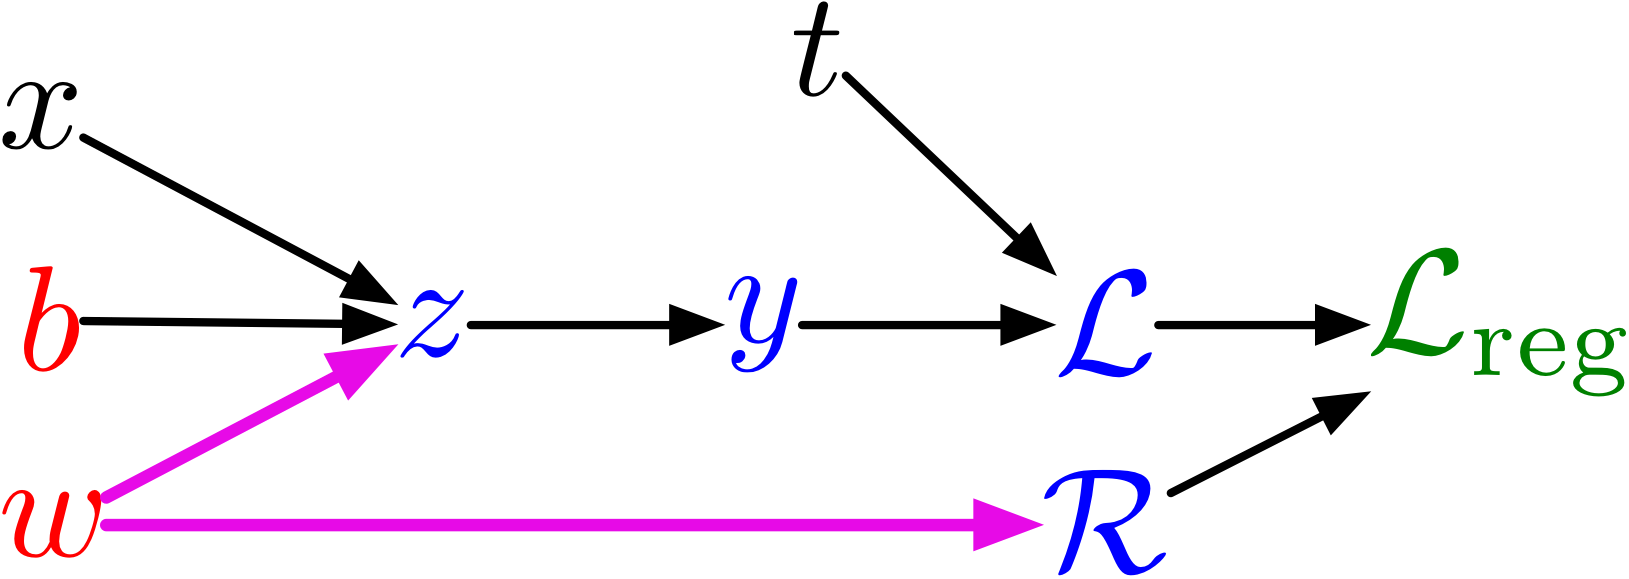
\includegraphics[width=0.9\linewidth]{pics/reg_computation_graph.png}

\end{minipage}\begin{minipage}{0.3\textwidth}
\centering
    \begin{align*}
      \intermediate &= \weightUni \inputUni + \bias \\
      \prediction &= \sigmoid(\intermediate) \\
      \loss &= \frac{1}{2} (\prediction - \target)^2 \\
      \regularizer &= \frac{1}{2} w^2 \\
      \loss_{\rm reg} &= \loss + \weightCost \regularizer
    \end{align*}
\end{minipage}
\end{frame}


\begin{frame}{Computation Graph has a Fan-Out $> 1$}
{\bf Softmax Regression}
\smallskip

\begin{minipage}{0.7\textwidth}
\centering
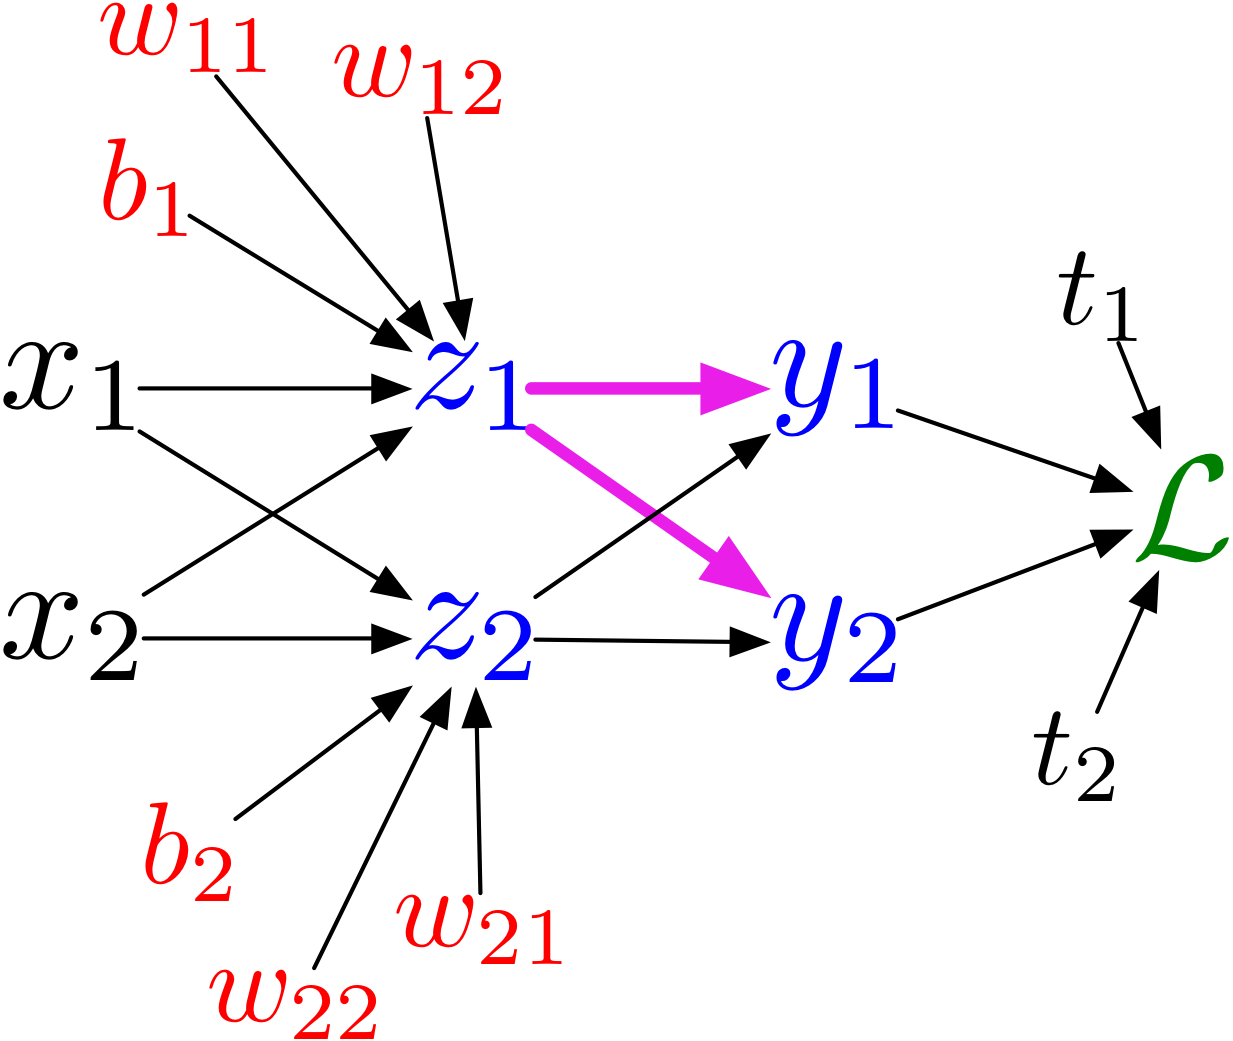
\includegraphics[width=0.7\linewidth]{pics/multiway_graph.png}

\end{minipage}\begin{minipage}{0.3\textwidth}
\centering
    \begin{align*}
      \intermediateK{\classIdxTwo} &= \sum_{\featIdx} \weightKJ{\classIdxTwo}{\featIdx} \inputJ{\featIdx} + \biasK{\classIdxTwo} \\[3mm]
      \predictionK{\classIdx} &= \frac{e^{\intermediateK{\classIdx}}}{\sum_{\classIdxTwo} e^{\intermediateK{\classIdxTwo}}} \\[5mm]
      \loss &= -\sum_{\classIdx} \targetK{\classIdx} \log \predictionK{\classIdx}
    \end{align*}
\end{minipage}
\end{frame}

\begin{frame}{Multi-variate Chain Rule}
Suppose we have functions $f(x, y)$, $x(t)$, and $y(t)$. 
      \begin{columns}
        \begin{column}{0.7 \linewidth}
          \[ \frac{\deriv}{\deriv t} f(x(t), y(t)) = \frac{\partial f}{\partial x} \frac{\deriv x}{\deriv t} + \frac{\partial f}{\partial y} \frac{\deriv y}{\deriv t} \]
        \end{column}
        \begin{column}{0.2 \linewidth}
          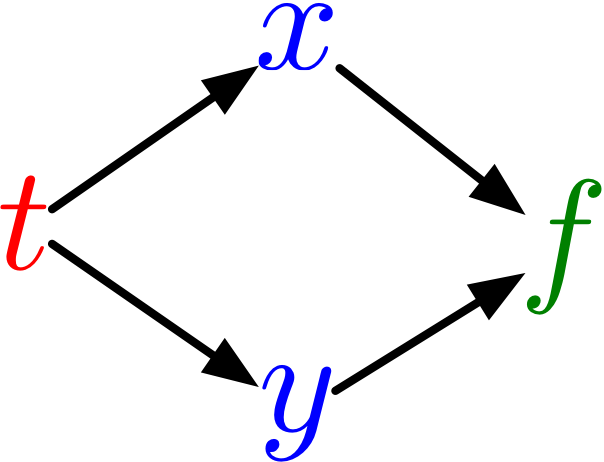
\includegraphics[width=\linewidth]{pics/toy_multivariate_graph.png}
        \end{column}
      \end{columns}

\vfill

Example:

\begin{minipage}{0.45\textwidth}
\centering
      \begin{align*}
        f(x, y) &= y + e^{xy} \\
        x(t) &= \cos t \\
        y(t) &= t^2
      \end{align*}
\end{minipage}\begin{minipage}{0.45\textwidth}
\centering
      \begin{align*}
        \frac{\deriv f}{\deriv t} &= \frac{\partial f}{\partial x} \frac{\deriv x}{\deriv t} + \frac{\partial f}{\partial y} \frac{\deriv y}{\deriv t} \\
        &= \left( y e^{xy} \right) \cdot \left( -\sin t \right) + \left( 1 + xe^{xy} \right) \cdot 2t
      \end{align*}
\end{minipage}
\end{frame}


\begin{frame}{Multi-variate Chain Rule}
In the context of back-propagation:
\vspace{1em}

\begin{minipage}{0.5\textwidth}

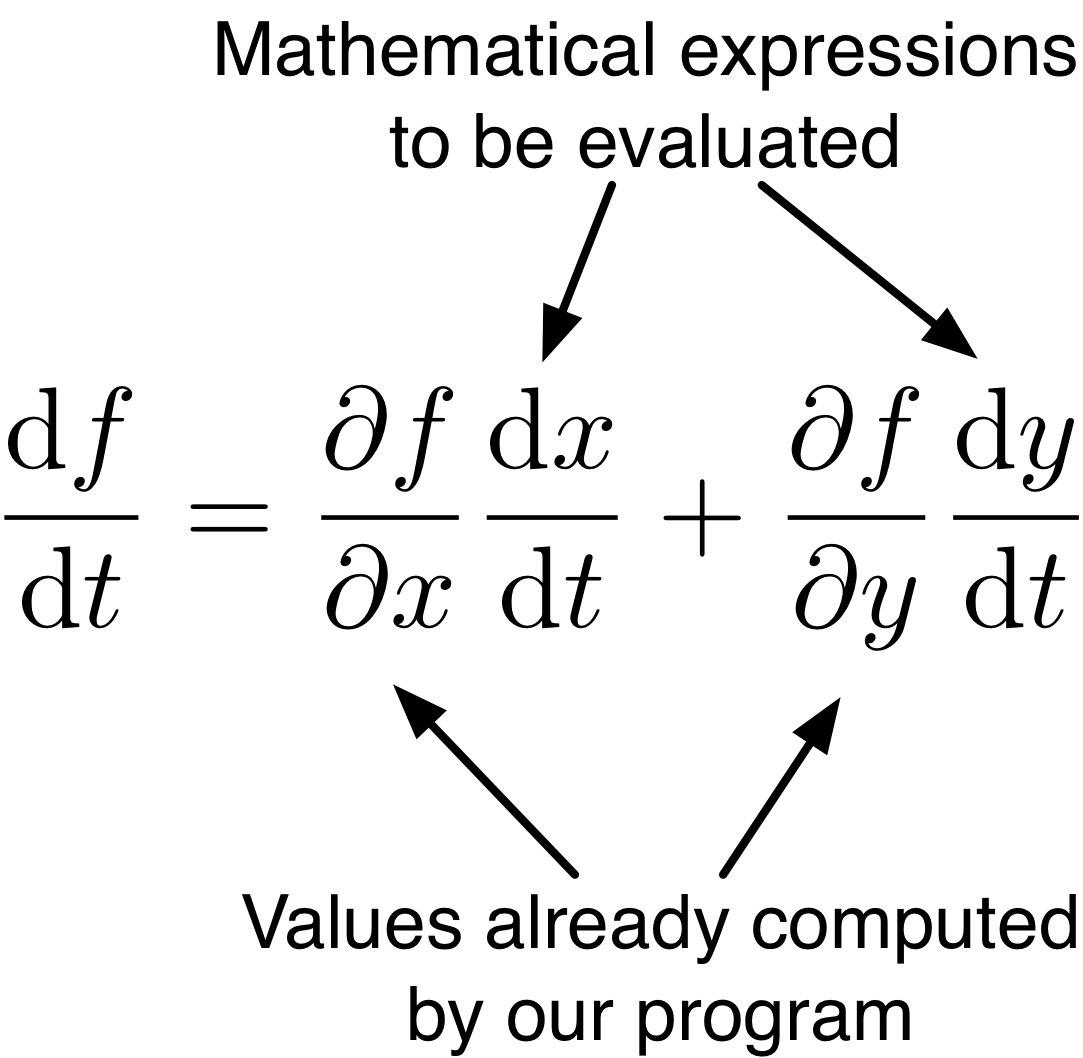
\includegraphics[width=0.7\linewidth]{pics/label_equation.png}

\end{minipage}\begin{minipage}{0.5\textwidth}

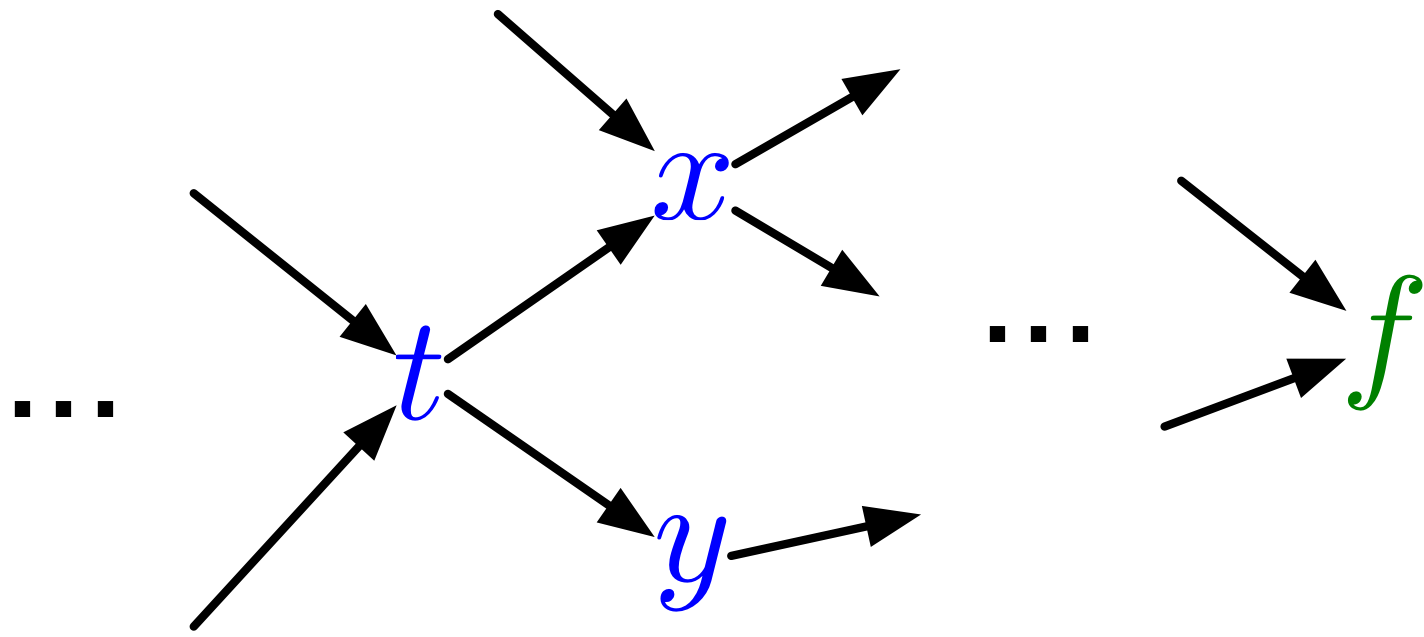
\includegraphics[width=1\linewidth]{pics/multivariate_context.png}
\end{minipage}

\vspace{1em}

In our new notation:\qquad \quad
 {\Large   $ \costDeriv{t} \;=\; \costDeriv{x} \, \frac{\deriv x}{\deriv t} + \costDeriv{y} \, \frac{\deriv y}{\deriv t} $}
\end{frame}





\begin{frame}{Backpropagation for Regularized Logistic Least Squares}
  \begin{columns}
    \begin{column}{0.35 \linewidth}
      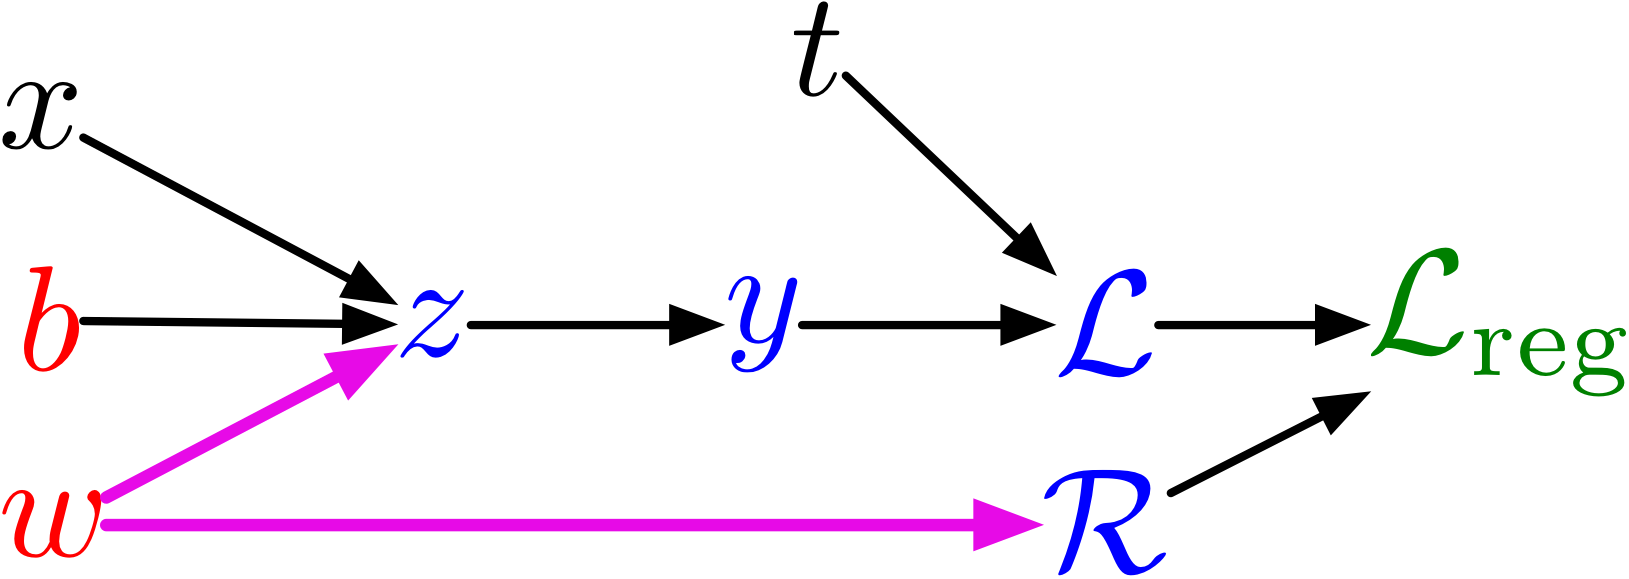
\includegraphics[width=\linewidth]{pics/reg_computation_graph.png}

      {\bf Forward pass:}
        \begin{align*}
          \intermediate &= \weightUni \inputUni + \bias \\
          \prediction &= \sigmoid(\intermediate) \\
          \loss &= \frac{1}{2} (\prediction - \target)^2 \\
          \regularizer &= \frac{1}{2} w^2 \\
          \loss_{\rm reg} &= \loss + \weightCost \regularizer
        \end{align*}

    \end{column}
    \pause
    \begin{column}{0.3 \linewidth}
      {\bf Backward pass:}
        \begin{align*}
          \costDeriv{\loss_{\rm reg}} &= 1 \\[4mm]
          \costDeriv{\regularizer} &= \frac{\deriv \loss_{\rm reg}}{\deriv \regularizer} = \weightCost  \\[4mm]
          \costDeriv{\loss} &= \frac{\deriv \loss_{\rm reg}}{\deriv \loss} = 1 \\[4mm]
          \costDeriv{\prediction} &= \costDeriv{\loss}\, \frac{\deriv \loss}{\deriv \prediction} = \costDeriv{\loss}\, (\prediction - \target) \\
        \end{align*}
    \end{column}
    \pause
    \begin{column}{0.35 \linewidth}
        \begin{align*}
          \costDeriv{\intermediate} &= \costDeriv{\prediction} \, \frac{\deriv \prediction}{\deriv \intermediate} = \costDeriv{\prediction} \, \logistic^\prime(\intermediate) \\[5mm]
          \textcolor[rgb]{0.9, 0, 0.9}{\costDeriv{\weightUni}} & \textcolor[rgb]{0.9, 0, 0.9}{= \costDeriv{\intermediate} \, \frac{\partial \intermediate}{\partial \weightUni} + \costDeriv{\regularizer} \frac{\deriv \regularizer}{\deriv \weightUni}}   \textcolor[rgb]{0.9, 0, 0.9}{= \costDeriv{\intermediate} \, \inputUni + \costDeriv{\regularizer} \, \weightUni } \\[5mm]
          \costDeriv{\bias} &= \costDeriv{\intermediate} \, \frac{\partial \intermediate}{\partial \bias} = \costDeriv{\intermediate}
        \end{align*}
    \end{column}
  \end{columns}
\end{frame}

\begin{frame}{Full Backpropagation Algorithm:}
  Let $v_1, \ldots, v_N$ be an ordering of the computation graph  where parents come before children (aka topological ordering). 

  % \begin{figure}
  %   \centering
  %   \includegraphics[width=0.3\linewidth,trim={0.3cm 4.5cm 1cm 4cm},clip]{pics/top_sort.jpg}
  % \end{figure}

  $v_N$ denotes the variable for which we try to compute gradients ($\loss$, $\loss_{\rm reg}$ etc).

  \begin{itemize}
  \item 
    forward pass:

    \begin{center}
      For $i = 1, \dots, N$, 

      Compute $v_i$ as a function of $\text{Parents}(v_i)$.
    \end{center}

  \item 
    backward pass:
$$\bar v_N=1$$
    \begin{center}
      For $i = N-1, \dots, 1$,
    \end{center}
    $$\bar{v_i} = \sum_{j \in \text{Children}(v_i)} \bar{v_j} \frac{\partial v_j}{\partial v_i}$$
  \end{itemize}
\end{frame}

%\begin{frame}{Computational Cost}
%  \begin{itemize}
%    \item Computational cost of forward pass: \\
%    \high{one add-multiply operation} per weight
%      \[ \intermediateK{\hidIdx} = \sum_{\featIdx} \weightLIJ{1}{\hidIdx}{\featIdx} \inputJ{\featIdx} + \biasLI{1}{\hidIdx} \]
%      %\pause
%    \item Computational cost of backward pass: \\
%    \high{two add-multiply operations} per weight
%      \begin{align*}
%        \costDeriv{\weightLIJ{2}{\outputIdx}{\hidIdx}} &= \costDeriv{\predictionK{\outputIdx}} \, \hiddenI{\hidIdx} \\
%        \costDeriv{\hiddenI{\hidIdx}} &= \sum_{\outputIdx} \costDeriv{\predictionK{\outputIdx}} \weightLIJ{2}{\outputIdx}{\hidIdx}
%      \end{align*}
%      %\pause
%    \item One backward pass is as expensive as two forward passes.
%    %\item For a multilayer perceptron, this means the cost is linear in the number of layers, quadratic in the number of units per layer.
%  \end{itemize}
%\end{frame}


\begin{frame}{Backpropagation}

  \begin{itemize}
  \item The algorithm for efficiently computing gradients in neural nets.\\[3mm]
  \item Gradient descent with gradients computed via backprop is used to train the overwhelming majority of neural nets today.\\[3mm]

  \item Even optimization algorithms much fancier than gradient descent (e.g.~second-order methods) use backprop to compute the gradients.
  
  %\item Despite its practical success, backprop is believed to be neurally implausible.
  \end{itemize}
\end{frame}

\begin{frame}{Auto-Differentiation}
	\begin{itemize}
		%\item Suppose we construct our networks out of a series of ``primitive'' operations (e.g., add, multiply) with specified routines for computing derivatives.
		\item \high{Autodifferentiation} performs backprop in a completely mechanical and automatic way.\\[3mm]
		\item Many autodiff libraries: PyTorch, Tensorflow, Jax, etc.\\[3mm]
		\item Although autodiff automates the backward pass for you, it's still important to know how things work under the hood.\\[3mm]
		\item In the tutorial, we will use an autodiff framework to build complex neural networks.
	\end{itemize}
\end{frame}


% \begin{frame}{ImageNet Results Over the Years}
  
% There are 1000 classes. Top-5 errors mean that the network can make 5 guesses for each image. So chance is 0.5\%.

%   \begin{center}
%   \begin{tabular}{llc}
%     {\bf Year} & {\bf Model} &  {\bf Top-5 error}\\
%     2010 & Hand-designed descriptors + SVM& 28.2\%\\
%     2011 & Compressed Fisher Vectors + SVM & 25.8\%\\
%     2012 & AlexNet & 16.4\% \\
%     2013 & a variant of AlexNet & 11.7\% \\
%     2014 & GoogLeNet & 6.6\% \\
%     2015 & deep residual nets  & 4.5\% \\
%   \end{tabular}
%   \end{center}

%   \vspace{1em}
%     Human-level performance is around 5.1\%. 

%     \vspace{1em}
% No longer running the object recognition competition \\
% because the performance is already so good.

% \end{frame}





\begin{frame}{Backpropagation for Two-Layer Neural Network}

  \begin{columns}
    \begin{column}{0.45 \linewidth}
      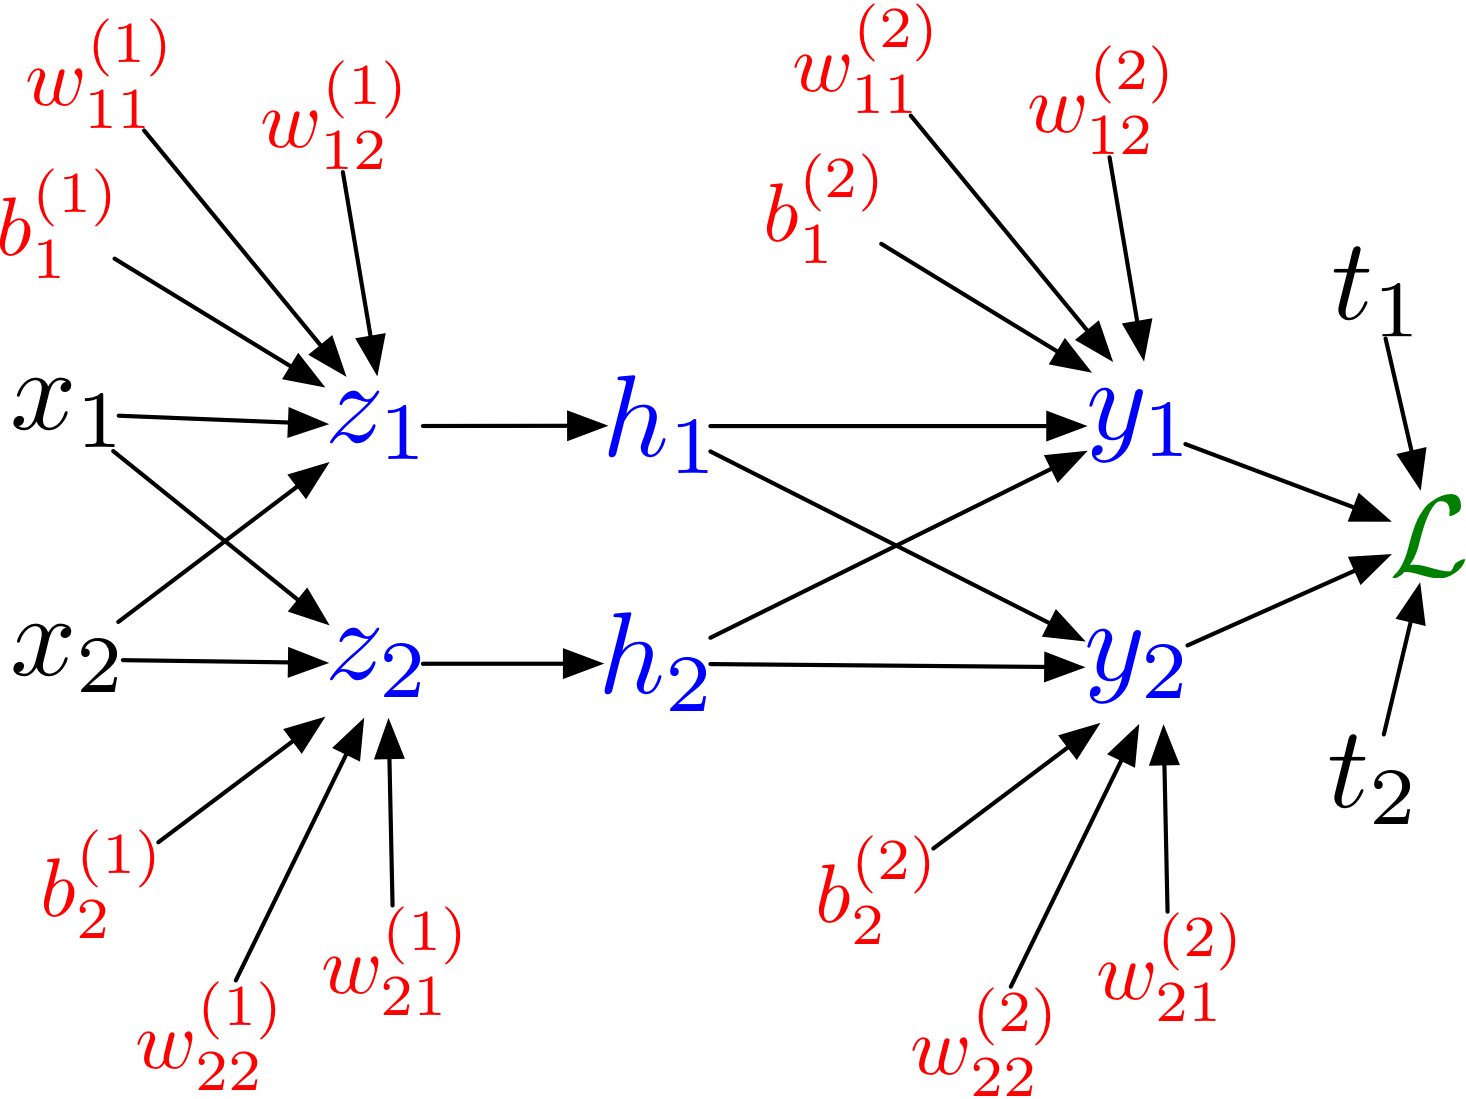
\includegraphics[width=0.9 \linewidth]{pics/mlp_graph.png}
      {\bf Forward pass:}
      \begin{align*}
        %\intermediates &= \weightMatL{1} \inputVec + \biasesL{1} \\
        %\hiddens &= \logistic(\intermediates) \\
        %\predictions &= \weightMatL{2} \hiddens + \biasesL{2} \\
        %\loss &= \| \targets - \predictions \|^2 \\
        \intermediateK{\hidIdx} &= \sum_{\featIdx} \weightLIJ{1}{\hidIdx}{\featIdx} \inputJ{\featIdx} + \biasLI{1}{\hidIdx}, \;\;\;
        \hiddenI{\hidIdx} = \logistic(\intermediateK{\hidIdx}) \\
        \predictionK{\outputIdx} &= \sum_{\hidIdx} \weightLIJ{2}{\outputIdx}{\hidIdx} \hiddenI{\hidIdx} + \biasLI{2}{\outputIdx}, \;\;\;\loss = \frac{1}{2} \sum_\outputIdx (\predictionK{\outputIdx} - \targetK{\outputIdx})^2
      \end{align*}
    \end{column}

    %\pause
    \begin{column}{0.45 \linewidth}
      {\bf Backward pass:}
      \begin{align*}
        \costDeriv{\loss} &= 1 \\
        \costDeriv{\predictionK{\outputIdx}} &= \costDeriv{\loss} \, (\predictionK{\outputIdx} - \targetK{\outputIdx}) \\
        \costDeriv{\weightLIJ{2}{\outputIdx}{\hidIdx}} &= \costDeriv{\predictionK{\outputIdx}} \, \hiddenI{\hidIdx} \\
        \costDeriv{\biasLI{2}{\outputIdx}} &= \costDeriv{\predictionK{\outputIdx}} \\
        \costDeriv{\hiddenI{\hidIdx}} &= \sum_{\outputIdx} \costDeriv{\predictionK{\outputIdx}} \weightLIJ{2}{\outputIdx}{\hidIdx} \\
        \costDeriv{\intermediateK{\hidIdx}} &= \costDeriv{\hiddenI{\hidIdx}} \, \logistic^\prime(\intermediateK{\hidIdx}) \\
        \costDeriv{\weightLIJ{1}{\hidIdx}{\featIdx}} &= \costDeriv{\intermediateK{\hidIdx}} \, \inputJ{\featIdx} \\
        \costDeriv{\biasLI{1}{\hidIdx}} &= \costDeriv{\intermediateK{\hidIdx}} 
      \end{align*}
    \end{column}
  \end{columns}

\end{frame}


\begin{frame}{Backpropagation for Two-Layer Neural Network}

  {\bf In vectorized form:}

  \vspace{1em}
  \begin{columns}
    \begin{column}{0.45 \linewidth}
    
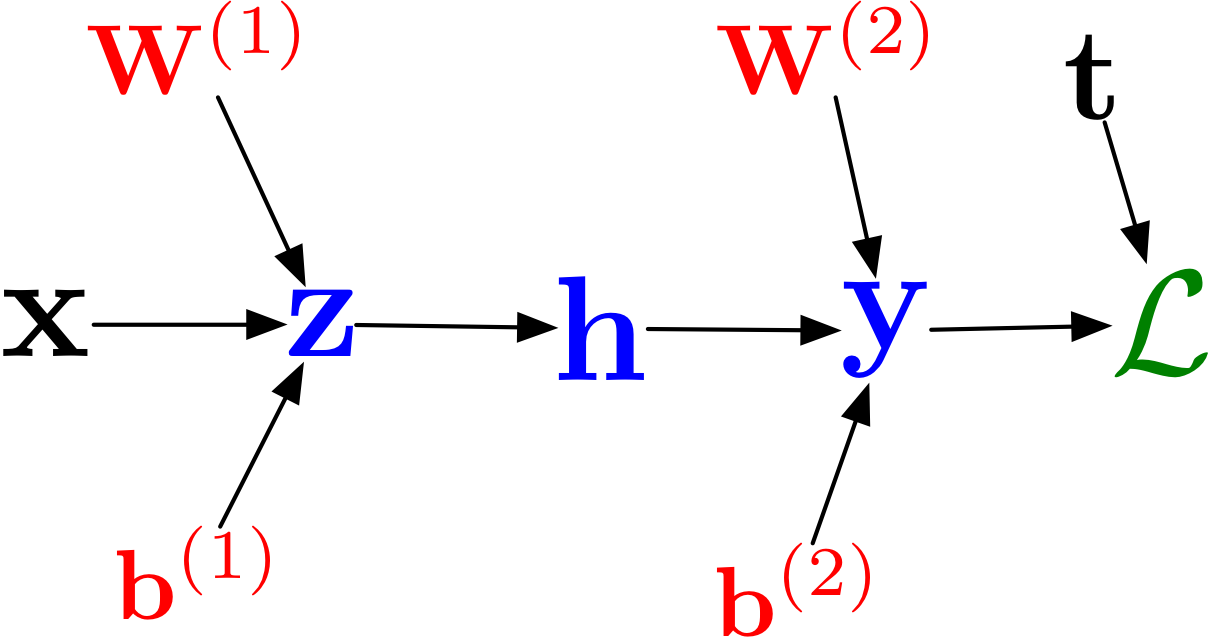
\includegraphics[width=0.9 \linewidth]{pics/mlp_graph_vectorized.png}

      {\bf Forward pass:}
      \begin{align*}
        \intermediates &= \weightMatL{1} \inputVec + \biasesL{1}, \;\;\;\hiddens = \logistic(\intermediates) \\
        \predictions &= \weightMatL{2} \hiddens + \biasesL{2},\;\;\;
        \loss = \frac{1}{2} \| \targets - \predictions \|^2
      \end{align*}     
    \end{column}

    \begin{column}{0.45 \linewidth}   
      {\bf Backward pass:}
      \begin{align*}
        \costDeriv{\loss} &= 1 \\
        \costDeriv{\predictions} &= \costDeriv{\loss} \, (\predictions - \targets) \\
        \costDeriv{\weightMatL{2}} &= \costDeriv{\predictions} \hiddens^\transpose \\
        \costDeriv{\biasesL{2}} &= \costDeriv{\predictions} \\
        \costDeriv{\hiddens} &= \weightMat^{(2) \transpose} \costDeriv{\predictions} \\
        \costDeriv{\intermediates} &= \costDeriv{\hiddens} \circ \logistic^\prime(\intermediates) \\
        \costDeriv{\weightMatL{1}} &= \costDeriv{\intermediates} \inputVec^\transpose \\
        \costDeriv{\biasesL{1}} &= \costDeriv{\intermediates}
      \end{align*}
      
    \end{column}
  \end{columns}
\end{frame}

\section{Autoencoders}


\begin{frame}{Non-linear Dimension Reduction}
  \begin{tabular}{ll}  
    \begin{tabular}{l}
      \!\!\!\!\!\!  \!\!\!\!\!\!       \!\!\!\!\!\!       \!\!\!\!\!\!       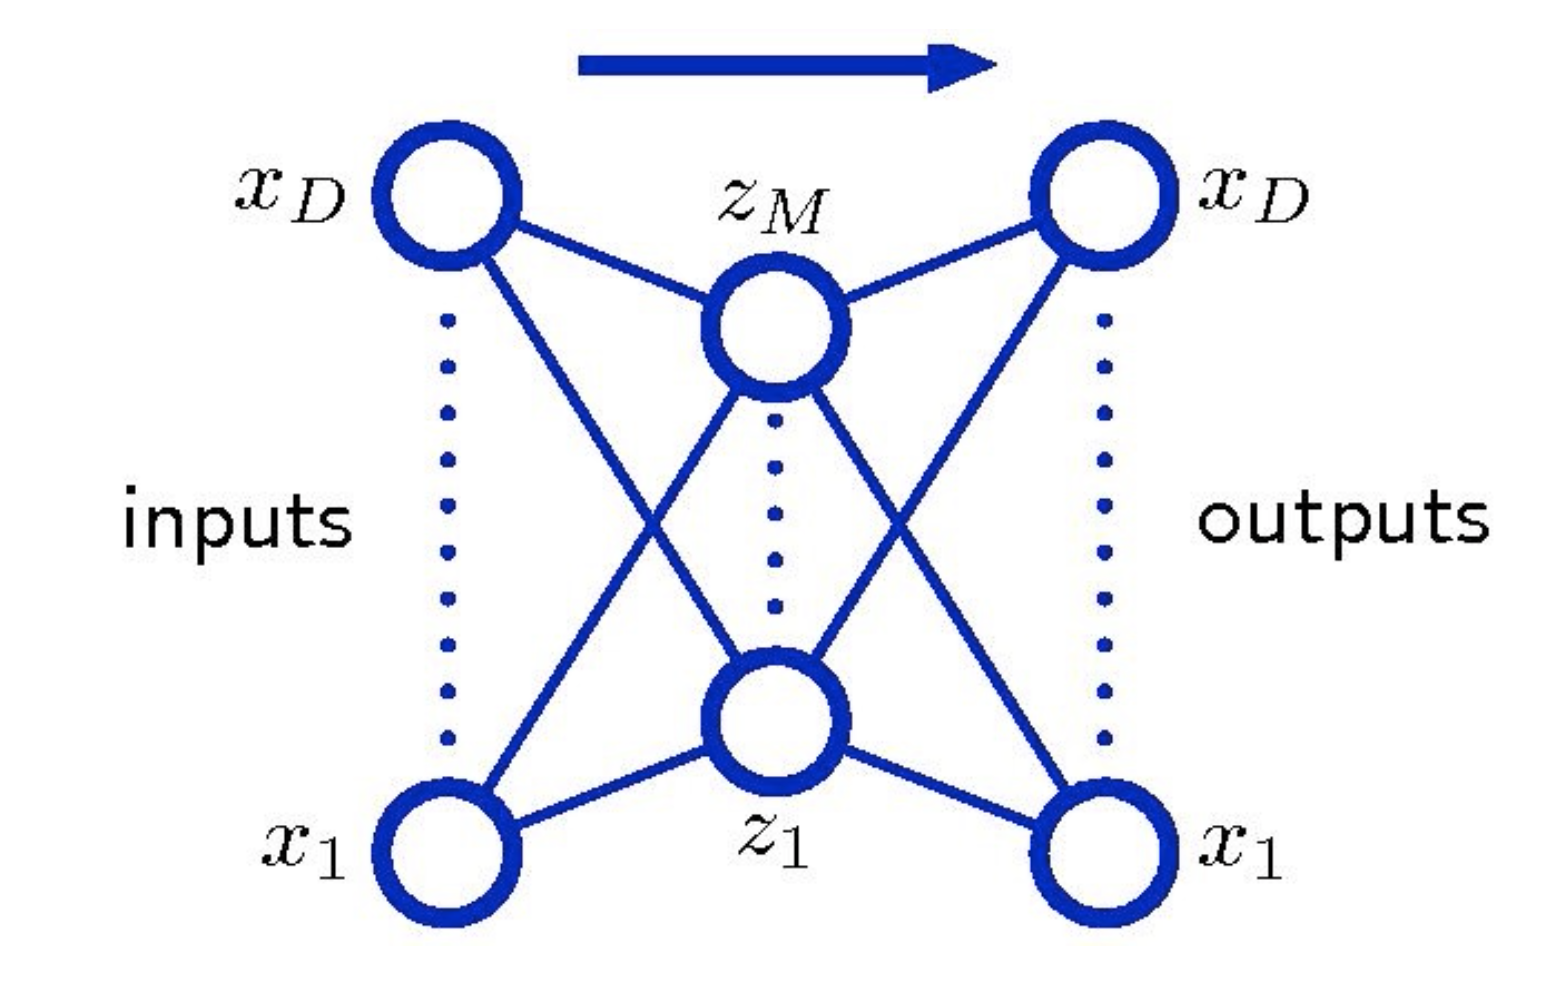
\includegraphics[width=1.9in]{pics/2-layer-auto-enc.png}
    \end{tabular}
    & \begin{tabular}{l}
        \hspace{-.4in} \parbox{.75\linewidth}{
        \begin{itemize}
        \item Neural networks can be used for \alert{nonlinear dimensionality reduction}.\\[3mm]
        \item This is achieved by having the same number of outputs as inputs. These models are called autoencoders.\\[3mm]
        \pause
        \item Consider a feed-forward neural network that has $D$ inputs, $D$ outputs, and $M$ hidden units, with $M<D$.\\[3mm]
        \item We can squeeze the information through a bottleneck.\\[3mm]
        \pause
        \item If we use a linear network (linear activation) this is very similar to Principal Components Analysis.
        \end{itemize}
        }
      \end{tabular}  
  \end{tabular}
\end{frame}


\begin{frame}
  \frametitle{Autoencoders and PCA}
  \begin{itemize}
  \item Given an input $\boldsymbol x$, its corresponding reconstruction is given by:
    $$
    y_k(\boldsymbol x, \boldsymbol w) = \sum_{j=1}^M w_{kj}^{(2)} \sigma\Big(\sum_{i=1}^D w_{ji}^{(1)}x_i \Big), \ \ \ k=1,...,D.
    $$
  \item We learn the parameters $\boldsymbol w$ by minimizing the reconstruction error:\\[-2mm]
    $$
    E(\boldsymbol w) = \frac{1}{2N} \sum_{n=1}^{N} \| y(\boldsymbol x_n, \boldsymbol w) - \boldsymbol x_n \|^2
    $$
  \end{itemize}
\pause
\vspace{-2mm}
  \begin{tabular}{ll}  
    \begin{tabular}{l}
      \!\!\!\!\!\! \!\!\!\!\!\! \!\!\!\!\!\! \!\!\!\!\!\!      \!\!\!\!\!\!       \!\!\!\!\!\!       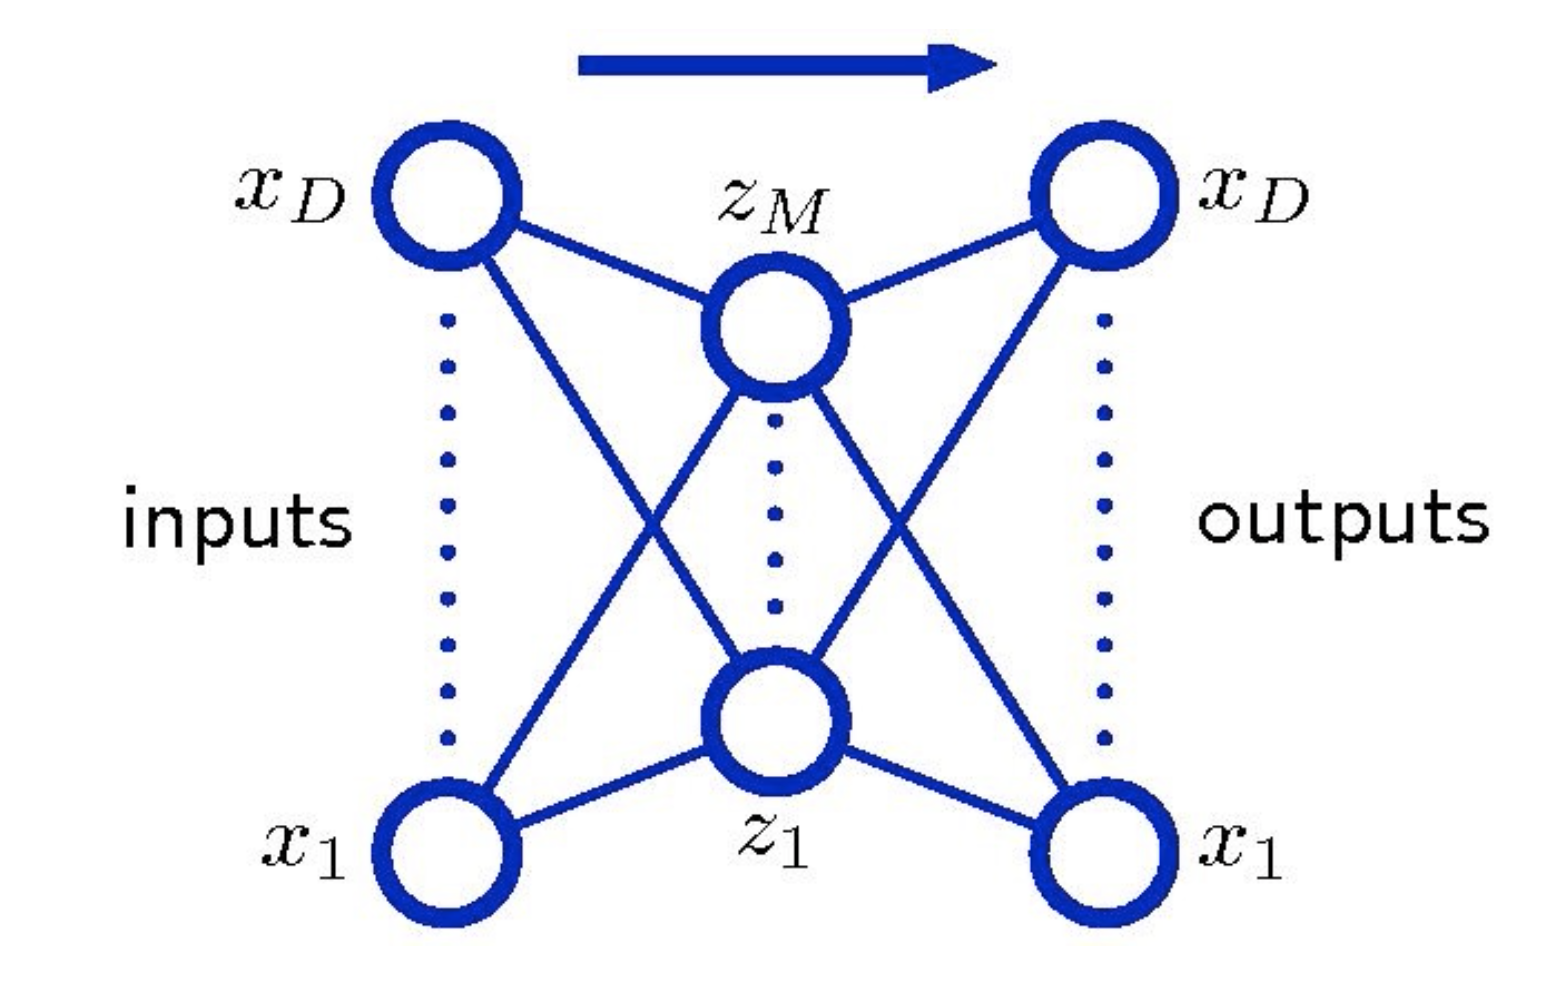
\includegraphics[width=1.99in]{pics/2-layer-auto-enc.png}
    \end{tabular}
    & \begin{tabular}{l}
        \hspace{-.4in} \parbox{.75\linewidth}{
        \begin{itemize}
        \item In the case when layers are linear:
        \begin{itemize}
        \item it will learn hidden units that are linear functions of the data and minimize squared error.
        \item $M$ hidden units will span the same space as the first $M$ principal components (PCA). 
        \end{itemize}      
        \end{itemize}
        }
      \end{tabular}  
  \end{tabular}
\end{frame}

\begin{frame}
  \frametitle{Deep Autoencoders }
  \begin{tabular}{ll}  
    \begin{tabular}{l}
      \!\!\!\!\!\!      \!\!\!\!\!\!       \!\!\!\!\!\!       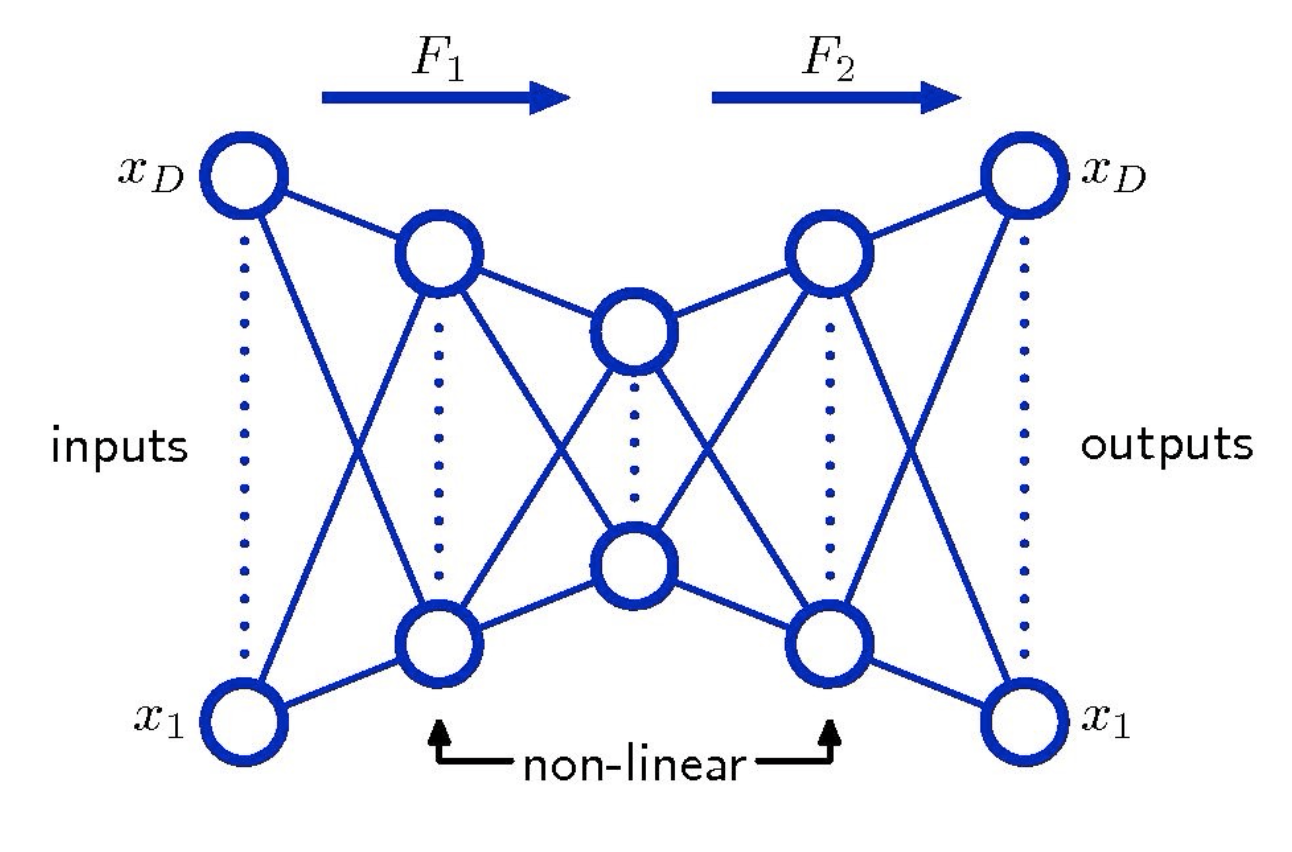
\includegraphics[width=1.99in]{pics/deep-auto-enc.png}
    \end{tabular}
    & \begin{tabular}{l}
        \hspace{-.4in} \parbox{.7\linewidth}{
        
        \begin{itemize}
        \item We can put extra nonlinear hidden layers between the input and the bottleneck and between the bottleneck and the output.
        \item This gives nonlinear generalization of PCA, providing non-linear dimensionality reduction.
\pause
        \item The network can be trained by the minimization of the reconstruction error function.
        \item Much harder to train.
          
        \end{itemize}

        }
      \end{tabular}  \\
  \end{tabular}
\end{frame}


\begin{frame}
  \frametitle{Geometrical Interpretation}

  \begin{itemize}
  \item Geometrical interpretation of the mappings performed by the network with 2 hidden layers for the case of $D=3$ and $M=2$ units in the middle layer.
    \begin{figure}
      \centering
      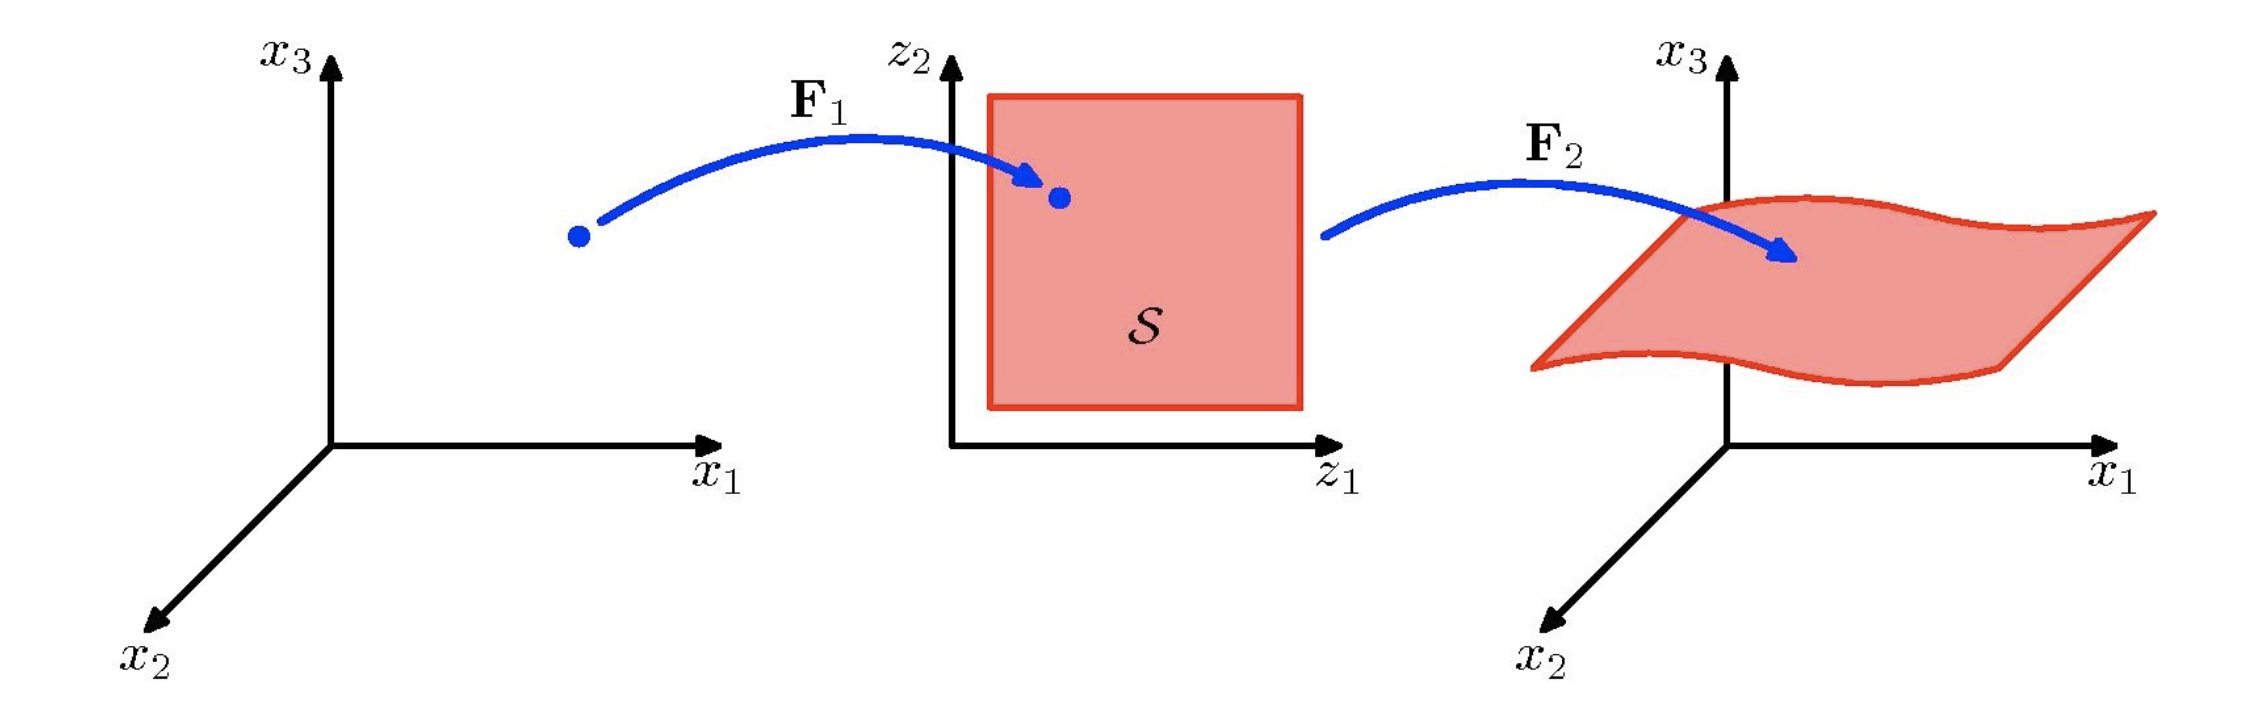
\includegraphics[width=3.99in]{pics/geo-inter.png}
    \end{figure}
  \item The mapping $F_1$ defines a nonlinear projection of points in the original $D$-space into the $M$-dimensional subspace.
  \item The mapping $F_2$ maps from an $M$-dimensional space into $D$-dimensional space.
  \end{itemize}
\end{frame}

\begin{frame}{Deep Autoencoders}
  \begin{tabular}{ll}  
    \begin{tabular}{l}
      \!\!\!\!\!\!      \!\!\!\!\!\!       \!\!\!\!\!\!       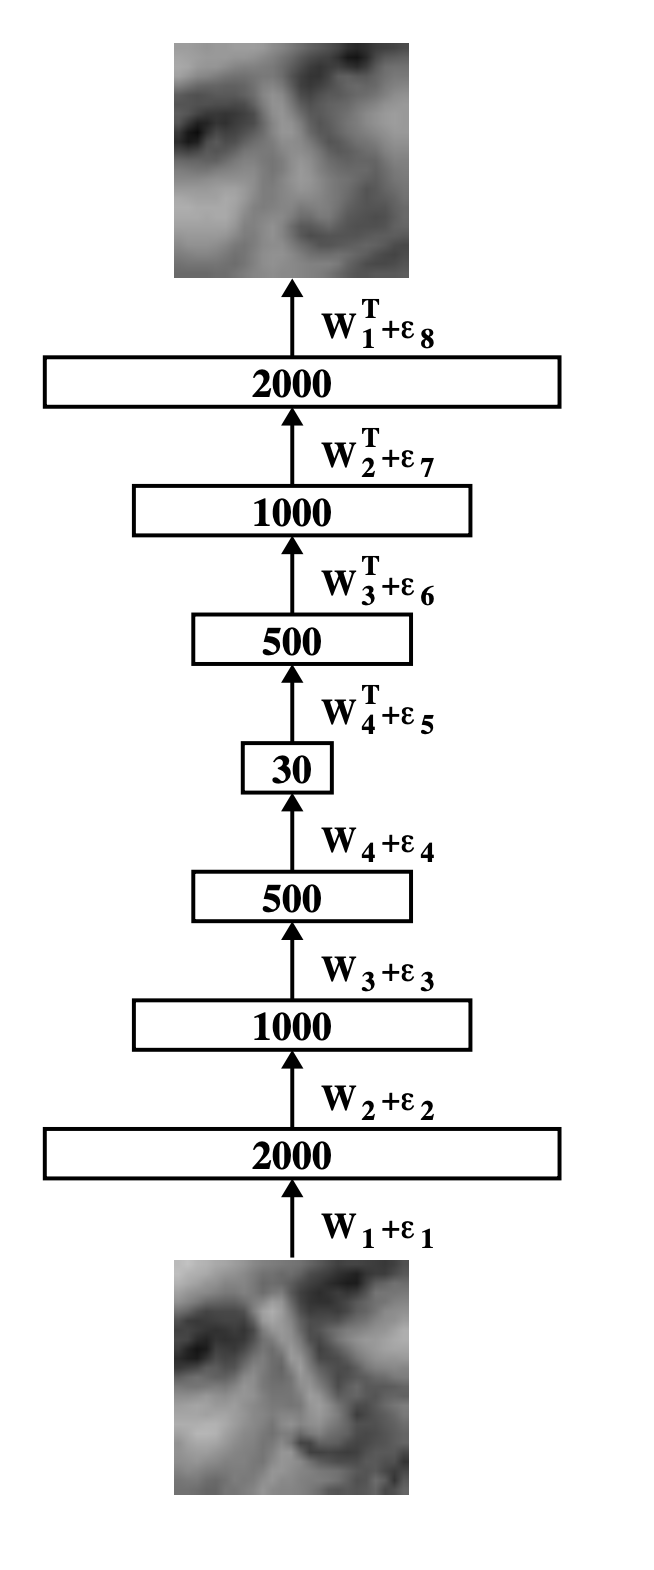
\includegraphics[width=0.99in]{pics/auto-enc-face.png}
    \end{tabular}
    & \begin{tabular}{l}
        \hspace{-.4in} \parbox{.7\linewidth}{
        
        \begin{itemize}
        \item[] \begin{figure}
            \centering
            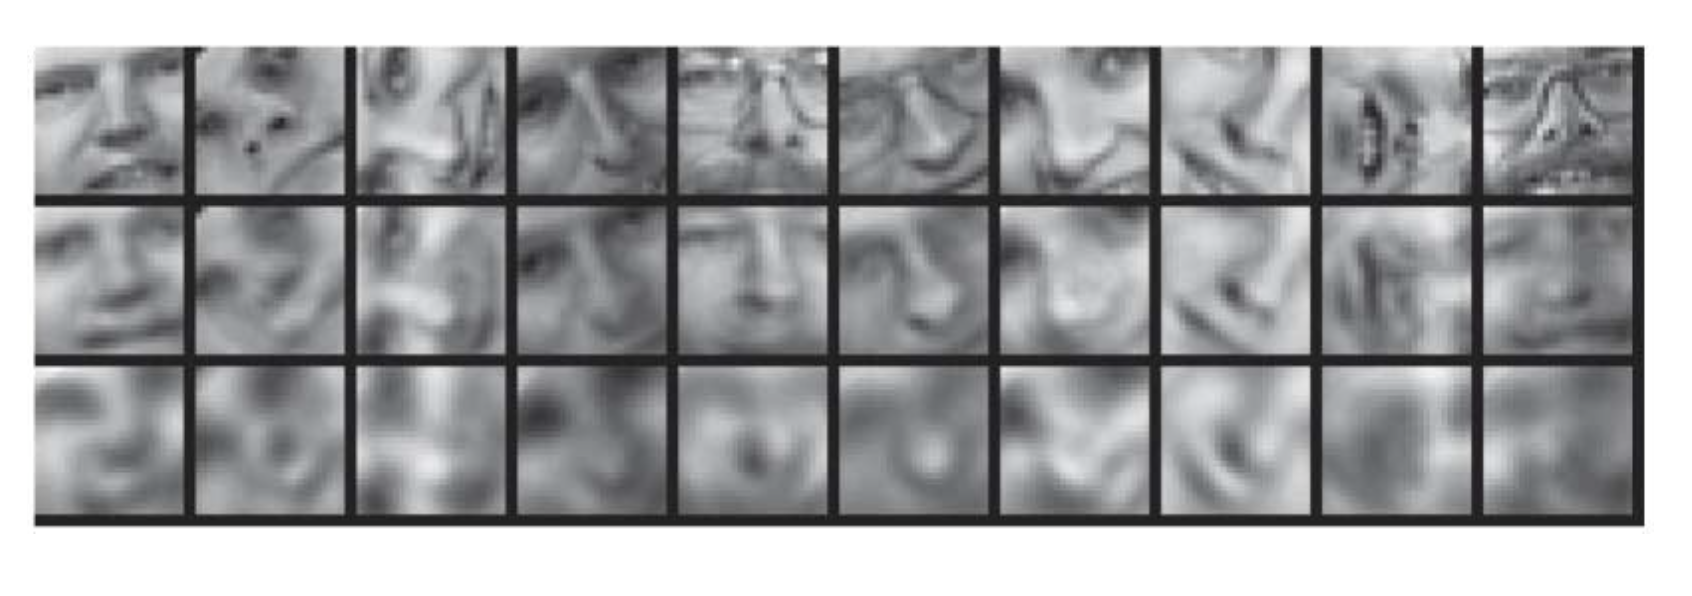
\includegraphics[width=2.99in]{pics/auto-enc-faces.png}
          \end{figure}
        \item We can consider very deep autoencoders.
%        \item There is an efficient way to learn these deep autoencoders.
        \item By row: Real data, Deep autoencoder with a bottleneck of 30 units, and 30-d PCA.      
        \end{itemize}
        }
      \end{tabular}  \\
  \end{tabular}
\end{frame}

\begin{frame}{Deep Autoencoders}
  \begin{itemize}
  \item Similar model for MNIST handwritten digits:
    \begin{figure}
      \centering
      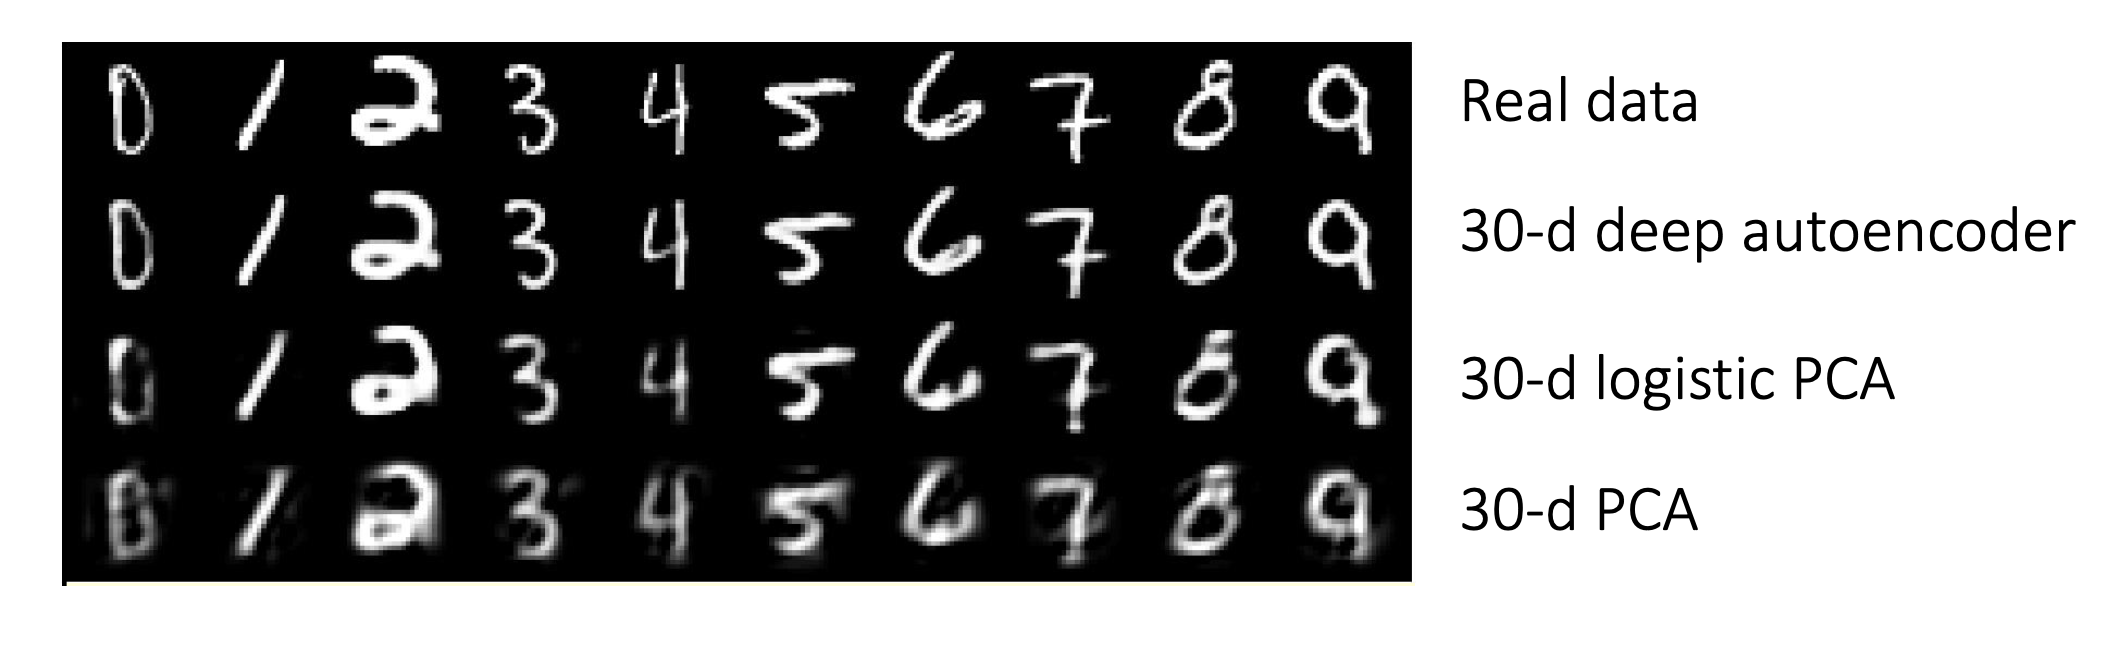
\includegraphics[width=3.99in]{pics/auto-enc-mnist.png}
    \end{figure}
  \item Deep autoencoders produce much better reconstructions.
  \end{itemize}
\end{frame}

\begin{frame}{Application: Image Denoising}
  \begin{figure}
  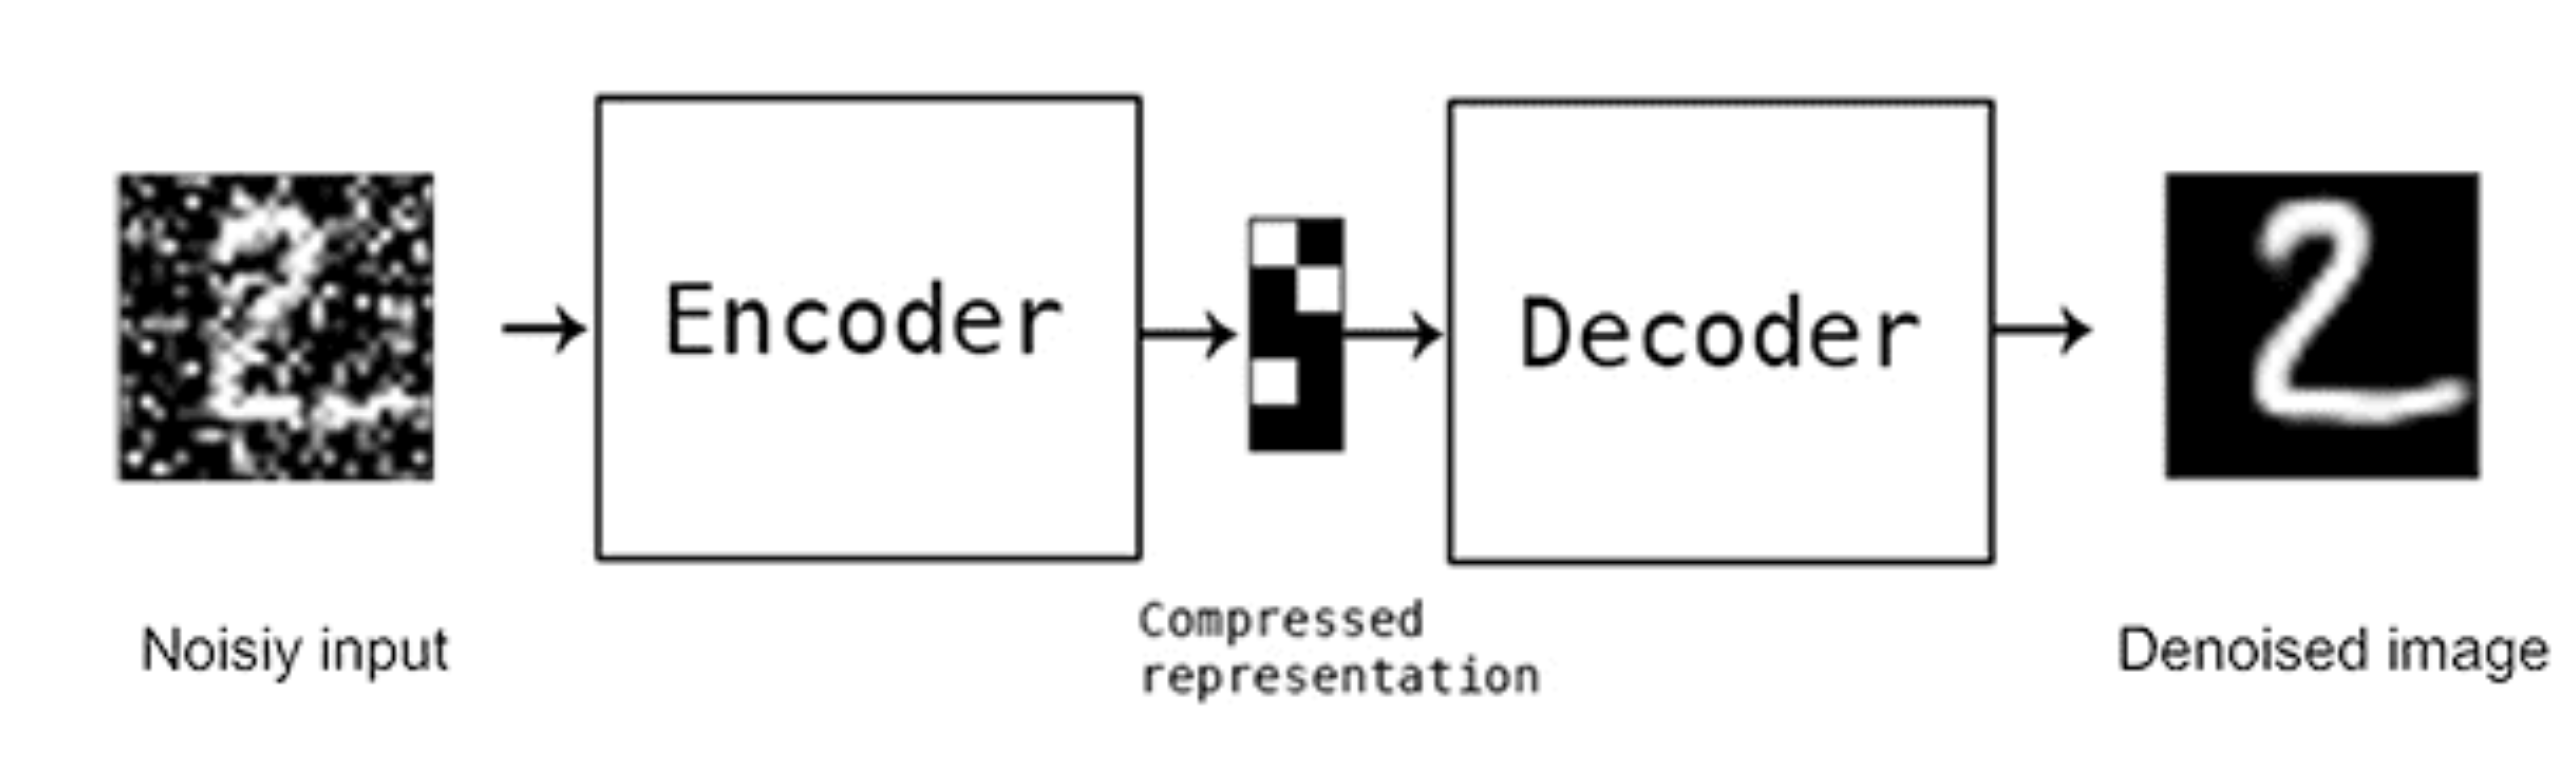
\includegraphics[width=4.5in]{pics/mnist-denoise}
  \end{figure}
  \vspace{-5mm}  
  \begin{itemize}
  \item We can train a \textbf{denoising autoencoder}.
  
  \item We feed noisy image as an input to the encoder 
  \item Minimize the reconstruction error between the decoder output and original image.
\item This method requires training and knowledge of the noise structure (fully supervised).
  
  \item In contrast, loopy BP works for a single noisy image and doesn't require the knowledge of noise structure (unsupervised).
    \end{itemize}
\end{frame}




\begin{frame}{Autoencoders: Summary}

  Autoencoders reconstruct their input via an encoder and a decoder.


  \begin{itemize}
  \item \textbf{Encoder}:  $e(x) = z \in F, \quad x \in X$

  \item \textbf{Decoder}:  $d(z) = \tilde x \in X$
  \item where  $X$ is the data space, and  $F$ is the feature (latent) space.
  

\item  $z$ is the code, 
\pause
 compressed representation of the input,  $x$. It is important that this code is a bottleneck, i.e. that
  $$
  \text{dim} \ F \ll \text{dim} \ X
  $$
\item Goal:
  $  \tilde x \;=\; d(e(x)) \;\approx\; x$.
\end{itemize}
\vspace{-9mm}\hspace{8mm}\qquad\qquad\qquad\qquad\qquad\qquad\qquad    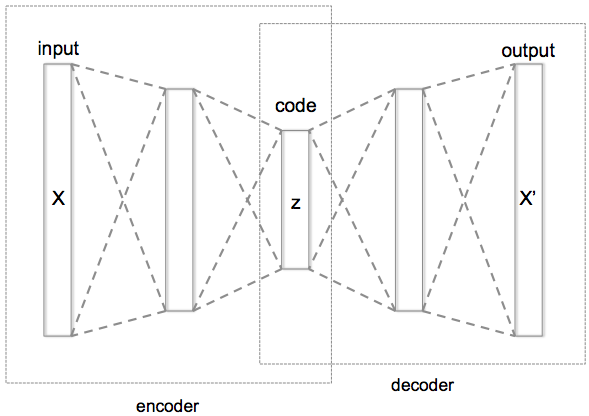
\includegraphics[width=1.8in]{pics/lecture_10_1.png}
\end{frame}


\begin{frame}
  \frametitle{Issues with (deterministic) Autoencoders}

  \begin{itemize}
  \item \textbf{Issue 1}: Proximity in data space does not mean proximity in feature space
    \begin{itemize}
    \item The codes learned by the model are deterministic, i.e.
      $$
      \begin{aligned}
        g(x_1) = z_1 \quad\Longrightarrow\quad f(z_1) = \tilde x_1 \\
        g(x_2) = z_2 \quad\Longrightarrow\quad f(z_2) = \tilde x_2 
      \end{aligned}
      $$

   \item but proximity in feature space is not ``directly'' enforced for inputs in close proximity in data space, i.e.
      $$
x_1 \approx x_2\quad\not\!\Longrightarrow  \quad     z_1 \approx z_2 
      $$

    \item The latent space may not be continuous, or allow easy interpolation.


    \end{itemize}
  \end{itemize}
\end{frame}


\begin{frame}
  \frametitle{Issues with (deterministic) Autoencoders}

  \begin{itemize}
  \item \textbf{Issue 1}: Proximity in data space does not mean proximity in feature space
    \begin{itemize}
    \item If the space has discontinuities (eg. gaps between clusters) and you sample/generate a variation from there, the decoder will simply generate an unrealistic output.

      \begin{figure}
      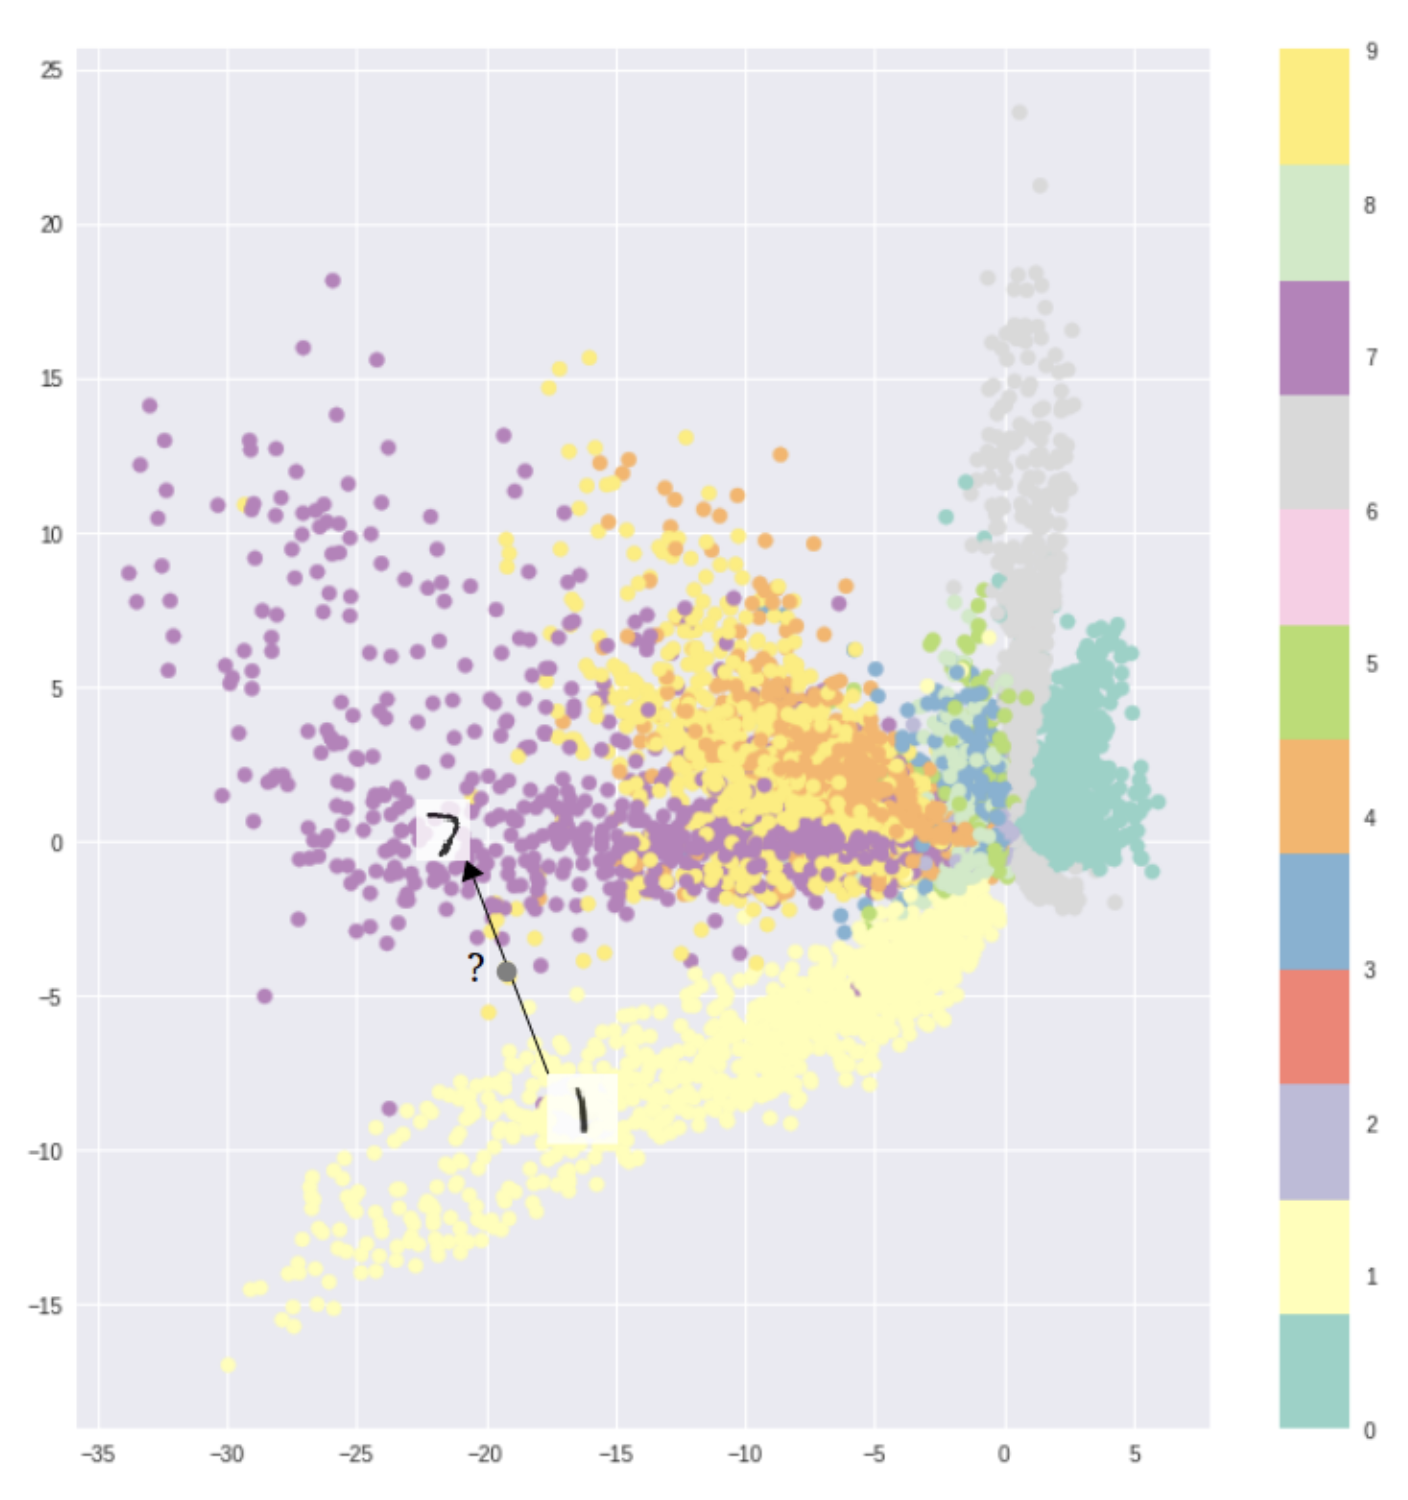
\includegraphics[width=1.9in]{pics/mnist-ae}
%        \includegraphics[width=4in]{pics/cluster-vae.png}  
      \end{figure}
    \end{itemize}
  \end{itemize}
  {\tiny Two dimensional latent space for the MNIST digit data.(Image credit: I.~Shafkat)}
\end{frame}


\begin{frame}
  \frametitle{Issues with (deterministic) Autoencoders}

  \begin{itemize}
  \item \textbf{Issue 2}: How to measure the goodness of a reconstruction?
    \begin{itemize}
    \item[] \begin{figure}
        \centering
        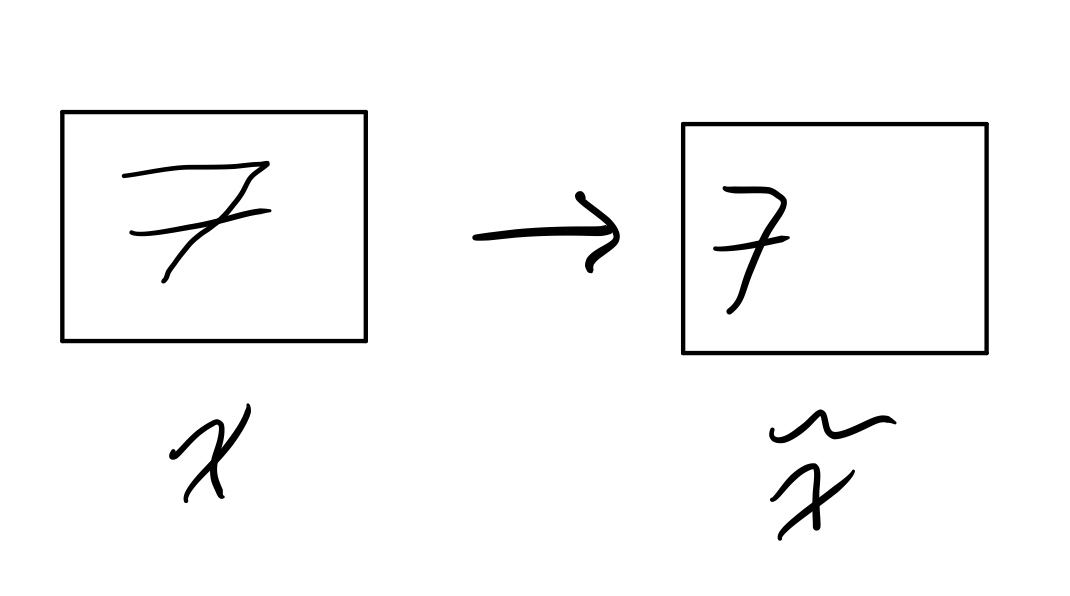
\includegraphics[width=2.1in]{pics/lecture_10_2.png}
      \end{figure}
    \item The reconstruction looks quite good. However, if we chose a simple distance metric between inputs and reconstructions, we would heavily penalize the left-shift in the reconstruction  $\tilde x$.
    \item Choosing an appropriate metric for evaluating model performance can be difficult, and that a miss-aligned objective can be disastrous.
    \end{itemize}
  \end{itemize}
\end{frame}

\begin{frame}
  \frametitle{Variational Autoencoders}
  \begin{itemize}
  \item Variational autoencoders (VAEs) encode inputs with uncertainty.\\[3mm]

  \item Unlike standard autoencoders, the encoder of a VAE outputs a probability distribution, $q_\phi(z )$ to approximate $p(z|x)$.\\[3mm]
  \item We assume that $q_\phi$ is a product of univariate normal distributions.
  \item Instead of the encoder learning an encoding vector, it learns two vectors: vector of means,  $\mu$, and another vector of standard deviations,  $\sigma$.

  \end{itemize}
\end{frame}


\begin{frame}
  \frametitle{Variational Autoencoders}
  \begin{itemize}

  \item The mean $\mu$ controls where encoding of input is centered while the standard deviation controls how much can the encoding vary.

    \begin{figure}
      \centering
      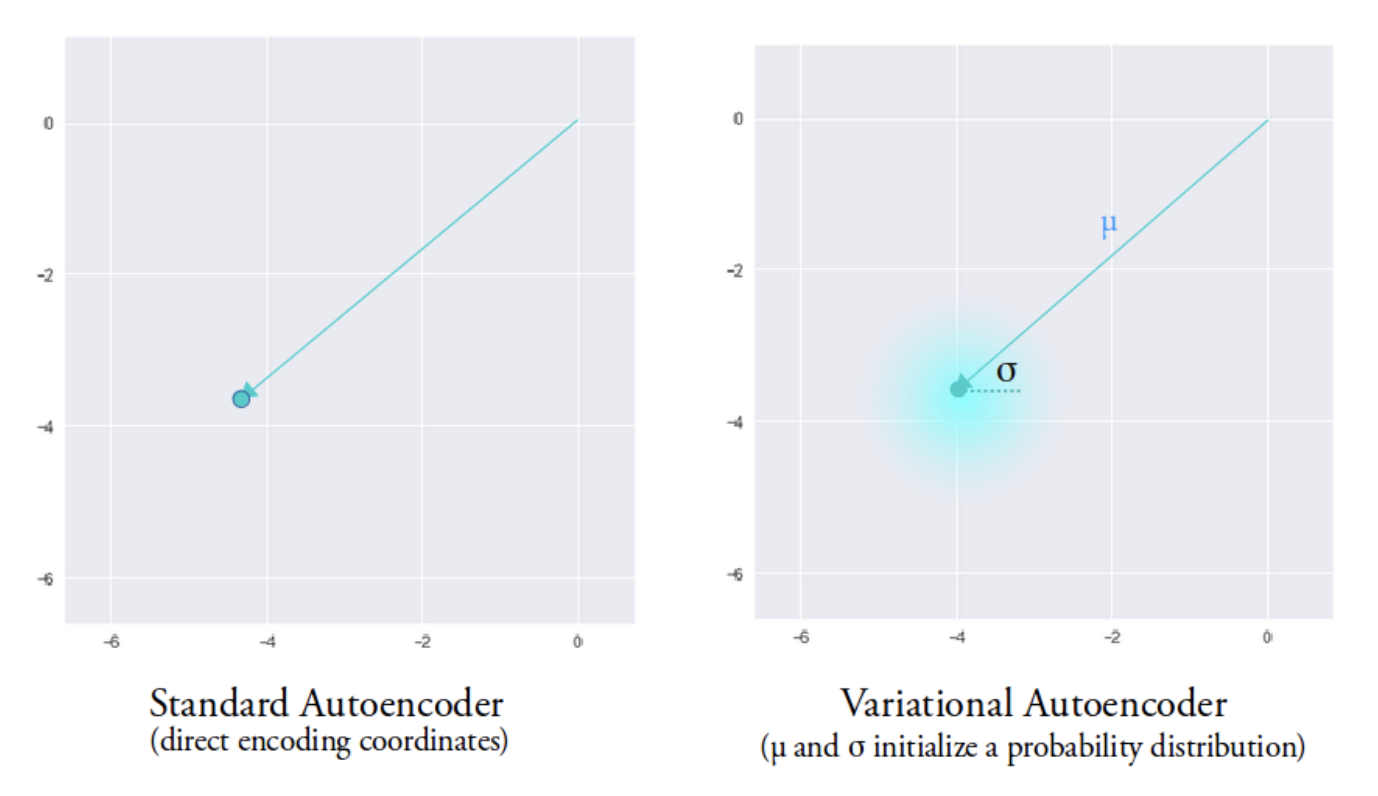
\includegraphics[width=2.5in]{pics/random-vae.png}{\tiny Image credit: I.~Shafkat}
    \end{figure}

  \item Encodings are generated at random from the ``ball'', the decoder learns that all nearby points refer to the same input. 
  \end{itemize}
  To minimize the reconstruction error, the algorithm may want to concentrate around the direct encodings. We will try to discourage this. 
\end{frame}



\begin{frame}
  \frametitle{VAE: Specifics}

  \begin{itemize}
  \item Our model is generated by the joint distribution over the latent codes and the input data  $p_\theta(x, z)$:
  \begin{itemize}
  \item The prior: $z\sim p_\theta(z)$ often Gaussian.
  \item The likelihood:  $x|z \sim {\rm Expfam}(x|d_{\theta}(z))$ with the {decoder}  $d_{\theta}(z)$ given by a DNN,
  \begin{itemize}
  \item e.g. for binary observations:  \;\;\; $p_\theta(x|z)\;=\;\prod_{d=1}^D {\rm Ber}(x_d|\sigma(d_{\theta}(z)))$
  \item e.g. for continuous observations: \;\;\;$p_\theta(x|z)\;=\;\prod_{d=1}^D N(x_d|d_{\theta}(z))$
  \end{itemize}
  \end{itemize} 
%Decomposing
%    $$
%    p(x, z) = \text{prior} \times \text{likelihood} = p(z)p(x | z)
%    $$
%    assuming our model looks like
%    \begin{figure}
%      \centering
%      \includegraphics[width=3.in]{pics/lecture_10_3.png}
%    \end{figure}

\item We could use the posterior $p_\theta(z|x) = p_\theta(x,z)/p_\theta(x)$ for encoding.
\end{itemize}
\pause
\begin{alertblock}{Issue: Learning
    $
    p(x) = \int p(x | z) p(z) dz
    $
    is intractable.}
	Introduce an approximation $q_\phi$ with its own set of parameters $\phi$, such that
    $$
    q_\phi (z|x) \;\approx\; p_\theta(z | x).
    $$

\end{alertblock}
%
%  \item However, learning
%    $
%    p(x) = \int p(x | z) p(z) dz
%    $
%    is intractable.
%    \item We introduce an approximation with its own set of parameters,  $q_\phi$, and learn these parameters such that
%    $$
%    q_\phi (z) \approx p(z | x).
%    $$
\end{frame}


\begin{frame}{After VAE is trained}

  \begin{itemize}
  \item Once a VAE is trained, we can sample new inputs (generative model)
    $$
z\sim p(z)\ \ \ \ \ \     \tilde x \sim p_\theta(x | z)
    $$

  \item We can also interpolate between inputs, using simple vector arithmetic.
    \begin{figure}
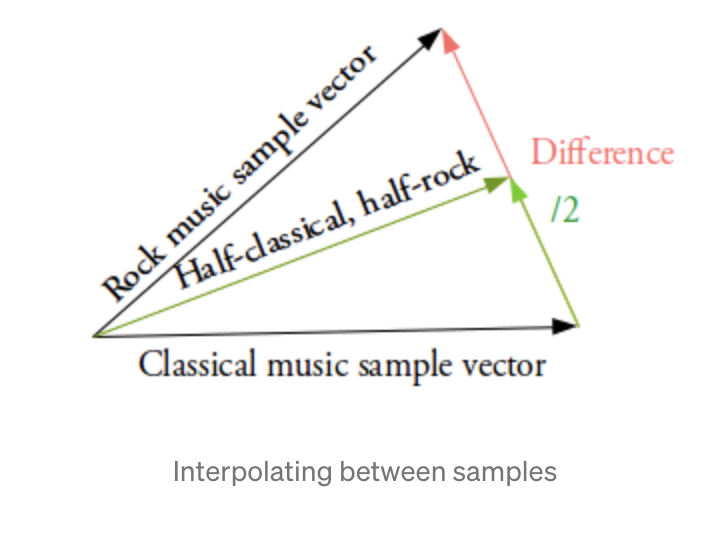
\includegraphics[width=3in]{pics/inter-vae.png}
    \end{figure}
  \end{itemize}
\end{frame}


%\begin{frame}
%  \frametitle{Example: MNIST}
%
%  \begin{itemize}
%  \item We choose the prior on $z$ to be the standard Gaussian
%    $$
%    p(z)\sim\mathcal{N}(0, I_M)
%    $$
%
%    \item our likelihood function to be
%    $$
%    p_\theta(x | z) = \text{Bernoulli}(\theta)
%    $$
%
%    \item and our approximate posterior is
%    $$
%    q_{\phi_i}(z | x_i) = \mathcal{N}(\mu_i, \sigma_i^2 I)
%    $$
%
%%  \item Finally, we use neural networks as our encoder and decoder
%%
%%    \begin{itemize}
%%    \item \textbf{Encoder}:  $g_\phi(x_i) = \phi_i = [\mu_i, \log \sigma_i]$
%%
%%\item \textbf{Decoder}:  $f_\theta(z_i) = \theta_i$
%%\item      where  $\theta_i$ are parameters of a Bernoulli rv for each input pixel.
%%
%%    \end{itemize}
%\item To get our reconstructed input, we simply evaluate
%    $$
%    \tilde x \sim p_{\theta}(x | z)
%    $$
%
%\item We will use neural networks as our encoder and decoder!
%  \end{itemize}
%\end{frame}

%\begin{frame}
%  \frametitle{Example: MNIST}
%
%  \begin{figure}
%    \centering
%    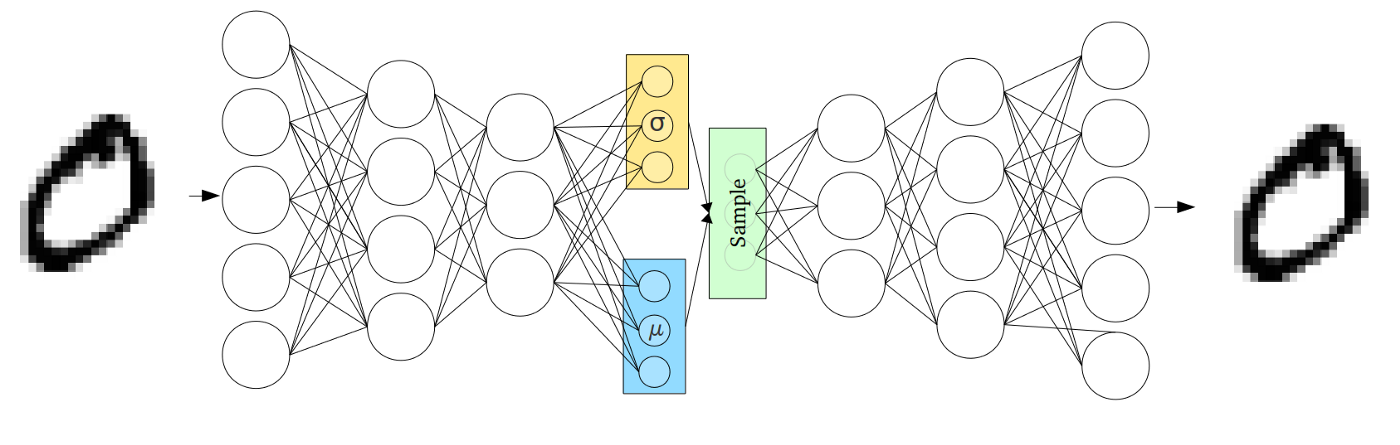
\includegraphics[width=3in]{pics/mnist-vae.png}
%  \end{figure}
%  
%  \begin{itemize}
%  \item Inputs  $x$ are encoded to $\mu$ and  $\log \sigma$, which parameterize  $q_\phi(z | x)$.
%  \item Before decoding, we draw a sample  $z \sim q_\phi(z | x) = \mathcal{N}(\mu, \sigma^2I)$ and evaluate its likelihood under the model with $p_\theta(x | z)$.
%    \item We compute the loss function  $\mathcal L(\theta, \phi ; x)$ and propagate its derivative with respect to $\theta$ and $\phi$,  $\nabla_\theta L$,  $\nabla_\phi L$, through the network during training. 
%  \end{itemize}
% \end{frame}


%\begin{frame}
%  \frametitle{The Reparametrization Trick}
%  
%  \begin{itemize}
%  \item Encoder generates a code by sampling from  $q_\phi(z | x)$.\\[3mm]
%  \item This sampling process introduces a major problem: gradients are blocked from flowing into the encoder, and hence it will not train.\\[3mm]
%  \item To solve this problem, we use the \textbf{reparameterization trick}.
%    \begin{itemize}
%    \item Instead of sampling  $z$ directly from its distribution (e.g.  $z_i \sim \mathcal{N}(\mu_i, \sigma_i^2)$) we express  $z_i$ as 
%      $$
%      z_i = \mu_i + \sigma_i \cdot \varepsilon_i \quad \text{where } \varepsilon_i \sim \mathcal N(0, I)
%      $$
%      with this, gradients can now flow through the entire network.
%
%    \end{itemize}
%
%  \end{itemize}
%\end{frame}










%\begin{frame}
%  \frametitle{Application: Image Denoising}
%  
%  \begin{figure}
%  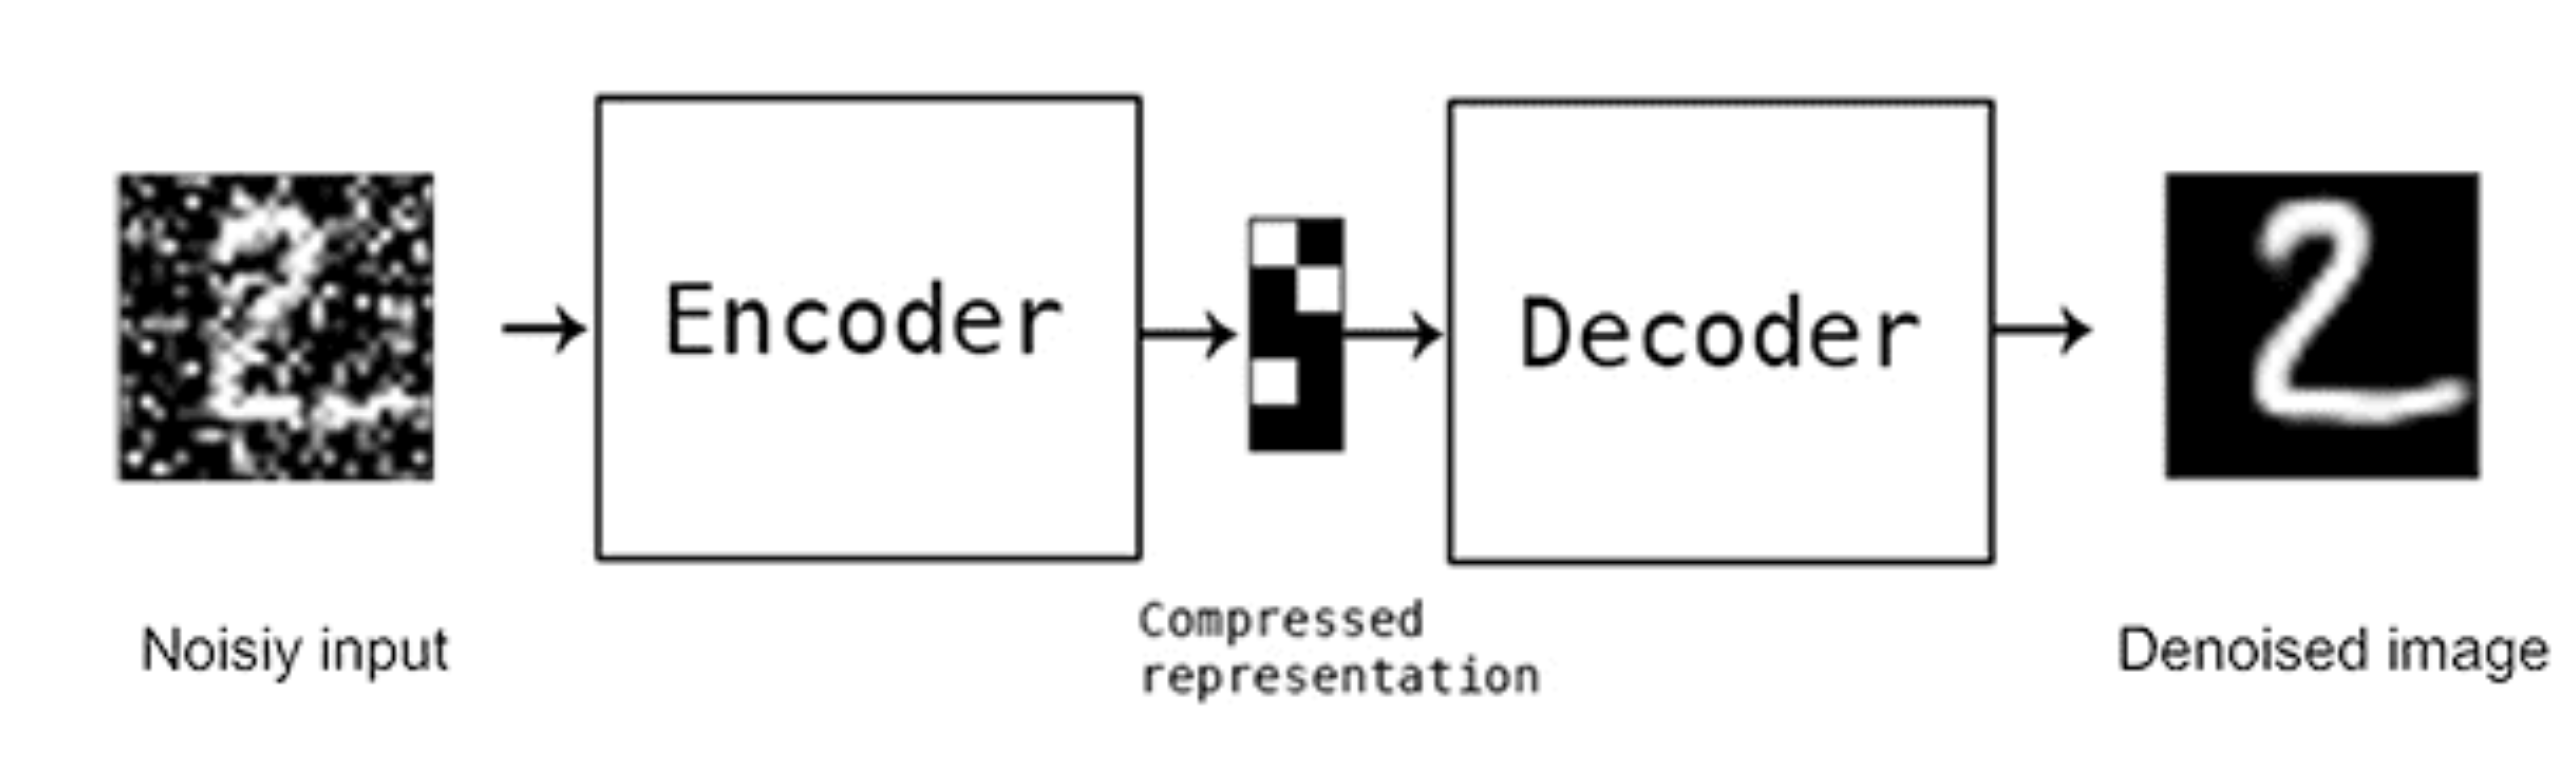
\includegraphics[width=4.5in]{pics/mnist-denoise}
%  \end{figure}
%  
%  \begin{itemize}
%\item This method requires training and knowledge of the noise structure (fully supervised).
%  
%  \item In contrast, loopy BP works for a single noisy image and doesn't require the knowledge of noise structure (unsupervised).
%  
%
%  
%    \end{itemize}
%
%
%\end{frame}





%\begin{frame}
%  \frametitle{VAE: Specifics}
%
%  \begin{itemize}
%  \item Our model is generated by the joint distribution over the latent codes and the input data  $p(x, z)$. Decomposing
%    $$
%    p(x, z) = \text{prior} \times \text{likelihood} = p(z)p(x | z)
%    $$
%    assuming our model looks like
%    \begin{figure}
%      \centering
%      \includegraphics[width=3.in]{pics/lecture_10_3.png}
%    \end{figure}

%\item The encoder is $p(z|x) = p(x,z)/p(x)$.
%\pause
%  \item However, learning
%    $
%    p(x) = \int p(x | z) p(z) dz
%    $
%    is intractable.
%    \item We introduce an approximation with its own set of parameters,  $q_\phi$, and learn these parameters such that
%    $$
%    q_\phi (z | x) \approx p(z | x).
%    $$
%
%  \end{itemize}
%\end{frame}

%\begin{frame}
%  \frametitle{Standard VAE}
%
%  \begin{itemize}
%  \item VI idea: we want to maximize $\log p(x)$ which
%    was lower bounded by the ELBO
%    $$
%    \begin{aligned}
%      \mathcal L(\theta, \phi ; x) =& \text{ELBO}\\
%      =&  \mathbb{E}_{z \sim q_\phi} \Big [ \log p_\theta({x | z}) \Big ] - D_{KL}(q_\phi(z | x) \| p(z)) 
%    \end{aligned}
%    $$
%which is the loss function we use when training VAEs.
%\pause
%\item First term is the expected log-likelihood and the second is the divergence of $q_\phi$ from  the true prior.
%\pause
%\item The encoder and decoder in a VAE become:
%%  \begin{itemize}
%%  \item \textbf{Encoder}:  $g(x_i) = \phi_i$
%%
%%    \item \textbf{Decoder}:  $f(z_i) = \theta_i$
%%  \end{itemize}
%  \begin{itemize}
%  \item \textbf{Encoder}:  $q_{\phi_i}(z|x_i) = \mathcal{N}(\mu_i,\sigma_i^2)$ where $\phi_i=(\mu_i,\log\sigma_i)$
%
%    \item \textbf{Decoder}:  $f(z) = \theta$ typically a neural network.
%  \end{itemize}
%
%\item The number of parameters for the encoder: $ N \times (|\mu_i| + |\sigma_i^2|)$
%  \end{itemize}
%\end{frame}


%\begin{frame}
%  \frametitle{Why VAE solves the problems of Autoencoders?}
%  \begin{itemize}
%  \item \textbf{Problem 1:} VAE generation model learns to reconstruct its inputs not only from the encoded points but also from the area around them.
%
%  \item \textbf{Problem 2:} The first term in the ELBO is the reconstruction log-likelihood, i.e. the log-likelihood that we would have re-constructed our data under our model. This serves as our measure of "goodness" of the reconstructed inputs.
%  \end{itemize}
%  
%\end{frame}



%\begin{frame}
%  \frametitle{Amortized Inference}
%
%  \begin{itemize}
%  
%  \item Instead of doing VI from scratch every time we see a new datapoint, we learn a function that can look at the data for a point $x_i$, and then output an approximate posterior $q_\phi(z_i|x_i)$.
%We call this a ``recognition model''.\\[3mm]
%
%\item Instead of a separate $\phi_i$ for each data example, we just have a single global $\phi$ that specifies the parameters of the recognition model.\\[3mm]
%
%\item Because the relationship between data and posteriors is complex and hard to specify by hand, we do this with a neural network!
%\item We can simply have a network take in $x_i$, and output the mean and variance vector for a Gaussian. The approximate posterior is given by
%$$q_\phi(z_i|x_i) = \mathcal{N}(z_i | \mu_\phi(x_i), \Sigma_\phi(x_i) )$$
%
%
%
%  \end{itemize}
%\end{frame}




%\begin{frame}
%  \frametitle{VAE vs Amortized VAE Pipeline}
%\begin{itemize}
%       \item For a given input (or minibatch) $x_i$,
%\end{itemize}
%
%
%  \begin{tabular}{ll}  
%    \begin{tabular}{l}
%    \parbox{.5\linewidth}{
%  \begin{itemize}
%  \item \textbf{Standard VAE}
%    \item Sample  $z_i \sim q_{\phi_i}(z | x_i) = \mathcal{N}(\mu_i,\sigma^2_iI)$.
%
%  \end{itemize}
%  }
%    \end{tabular}
%    & \begin{tabular}{l}
%    \hspace{-.5in}
%\parbox{.5\linewidth}{
%  \begin{itemize}
%    \item \textbf{Amortized VAE}
%    \item Sample  \\$z_i\! \sim\! q_{\phi}(z | x_i)\!=\!\mathcal{N}(\mu_\phi(x_i), \Sigma_\phi(x_i))\!\!\!$
%  \end{itemize}
%        }
%      \end{tabular}  \\
%  \end{tabular}
%\begin{itemize}
%    \item Run the code through decoder and get likelihood:  $p_\theta(x| z)$.
%    \item Compute the loss function:  $L(x ; \theta, \phi) = - E_{z_\phi \sim q_\phi} \Big [ \log p_\theta({x | z}) \Big ] + {KL}(q_\phi(z | x) \| p(z))$
%
%       \item Use gradient-based optimization to backpropagate  $\nabla_\theta L$,  $\nabla_\phi L$
%       \item This allows us to use the share parameters for all data points, and reduce the number of parameter for the encoder to that of the encoding NN.
%
%\item Standard VAE is more expressive as no parameters are shared across different data points.
%
%\end{itemize}
%\end{frame}


%\begin{frame}
%  \frametitle{Standard vs Amortized VAE}
%
%  \begin{itemize}
%
%\item This allows us to use the share parameters for all data points, and reduce the number of parameter for the encoder to that of the encoding NN.
%
%\item Standard VAE encoder is more expressive since no parameters are shared across different data points.
%  \end{itemize}
%\end{frame}
%
\begin{frame}{Example: MNIST}

  \begin{itemize}
  \item We choose the prior on $z$ to be the standard Gaussian:\;\;\;
    $
    p(z)\sim\mathcal{N}(0, I).
    $\\[3mm]

    \item The likelihood function:\;\;\;
    $
    p_\theta(x | z) = \prod_{i=1}^D\text{Bernoulli}(\theta_i).
    $\\[3mm]

    \item Approximate posterior:\;\;\;
    $
    q_{\phi}(z | x) = \mathcal{N}(\mu_\phi(x), \Sigma_\phi(x))
    $, where $\Sigma_\phi$ diagonal.\\[3mm]

  \item Finally, we use neural networks as our encoder and decoder
    \begin{itemize}
    \item \textbf{Encoder}:  $e_\phi(x) =  [\mu_\phi(x), \log \Sigma_\phi(x)]$
\item \textbf{Decoder}:  $d_\theta(z) = (\theta_1(z),\ldots,\theta_d(z))$
\item      where  $\theta_i$ are parameters of a Bernoulli rv for each input pixel.
    \end{itemize}
\item To get our reconstructed input, we simply take
    $$
    \tilde x \sim p_{\theta}(x | z)
    $$
  \end{itemize}
\end{frame}



\begin{frame}
  \frametitle{Example: MNIST}

  \begin{figure}
    \centering
    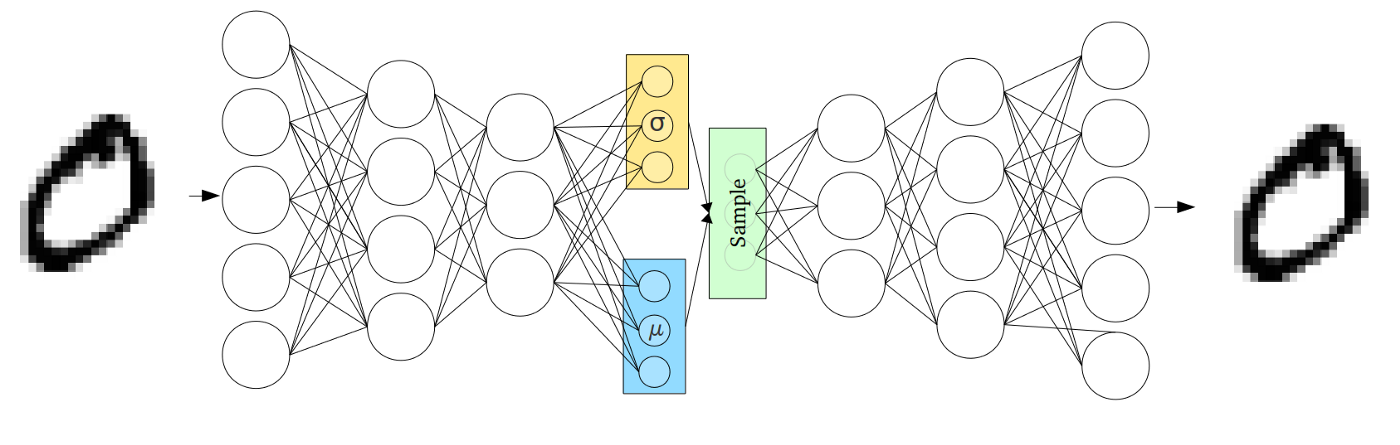
\includegraphics[width=4in]{pics/mnist-vae.png}
  \end{figure}
  
  \begin{itemize}
  \item We use neural networks for both the encoder and the decoder.
    \item We compute the loss function  $\mathcal L(\theta, \phi ; x)$ and propagate its derivative with respect to $\theta$ and $\phi$,  $\nabla_\theta \mathcal L$,  $\nabla_\phi \mathcal L$, through the network during training. 
    \item We use reparametrization trick as described before.
  \end{itemize}
 \end{frame}



\begin{frame}
  \frametitle{MNIST: Autoencoder vs VAE}

Codes generated by L: AE R: VAE
\begin{figure}
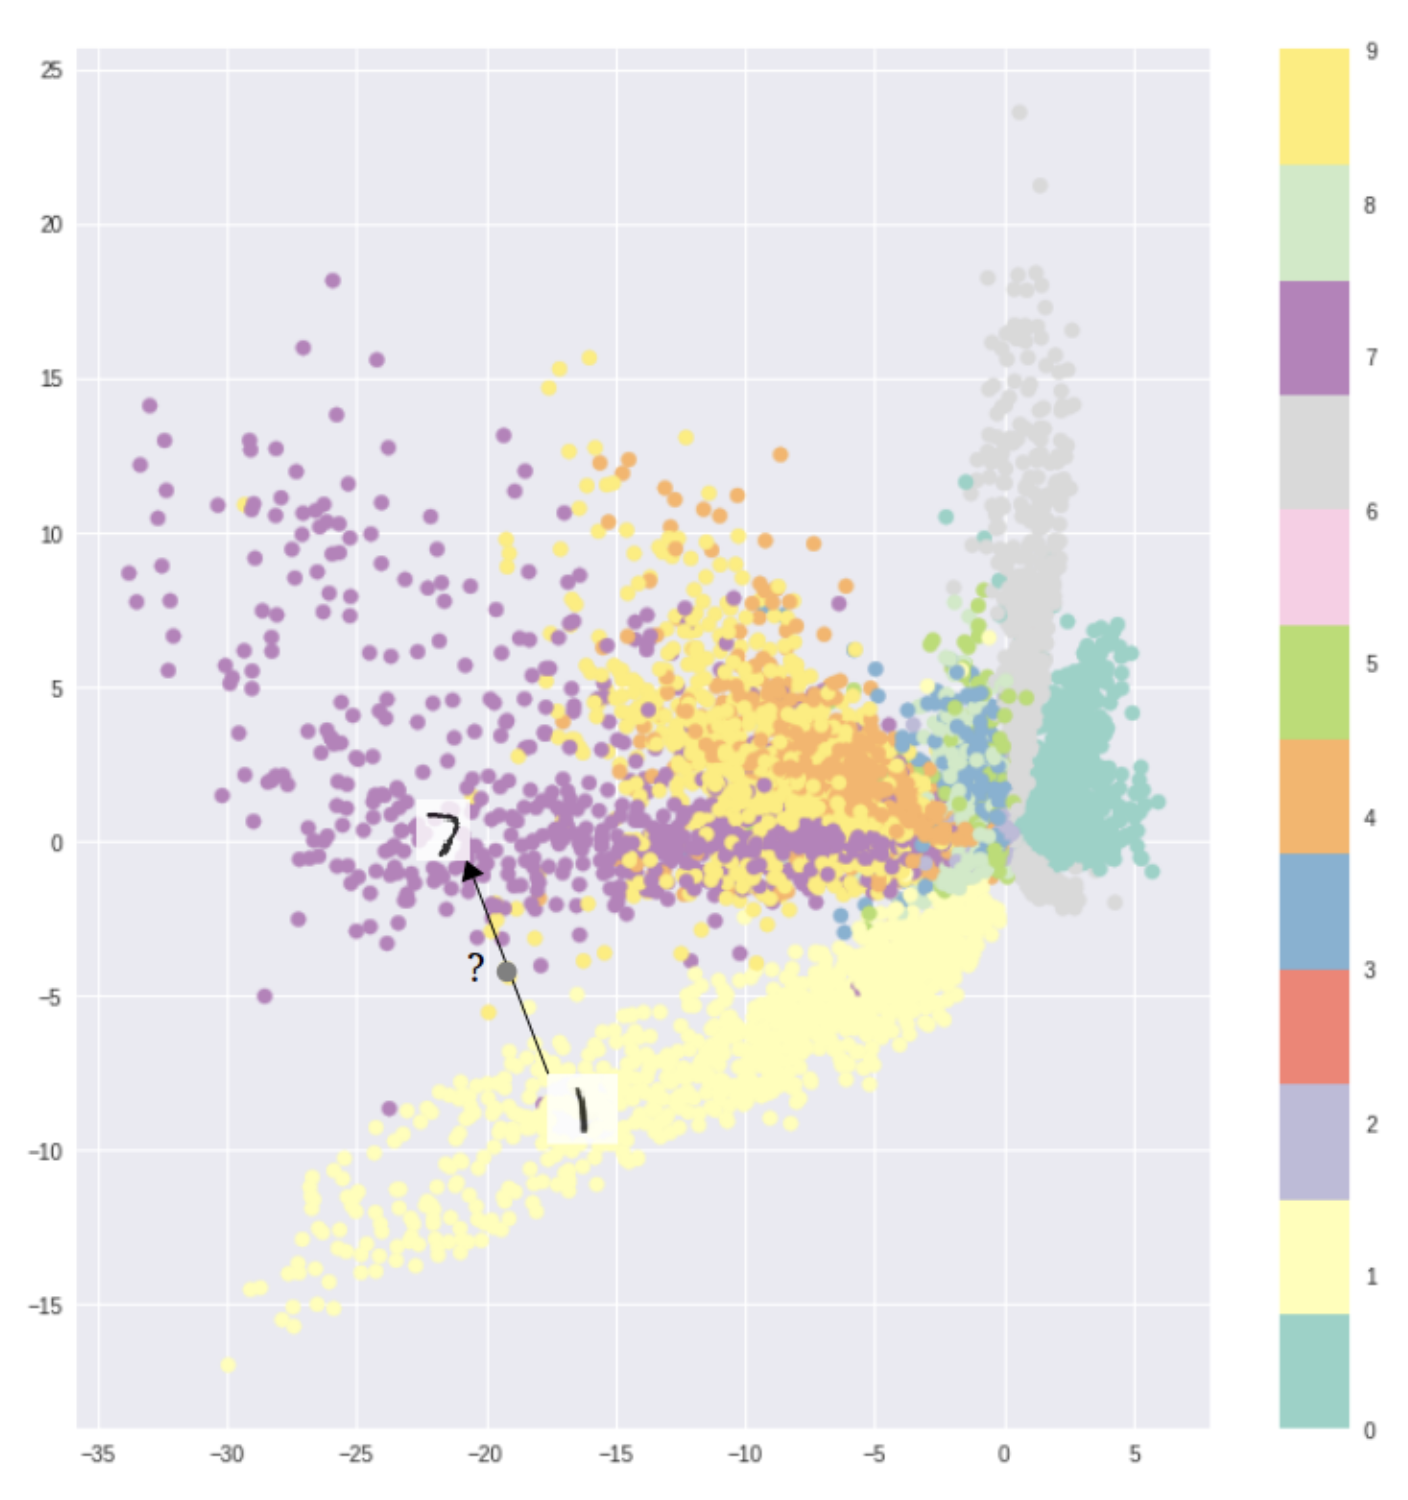
\includegraphics[width=2in]{pics/mnist-ae}
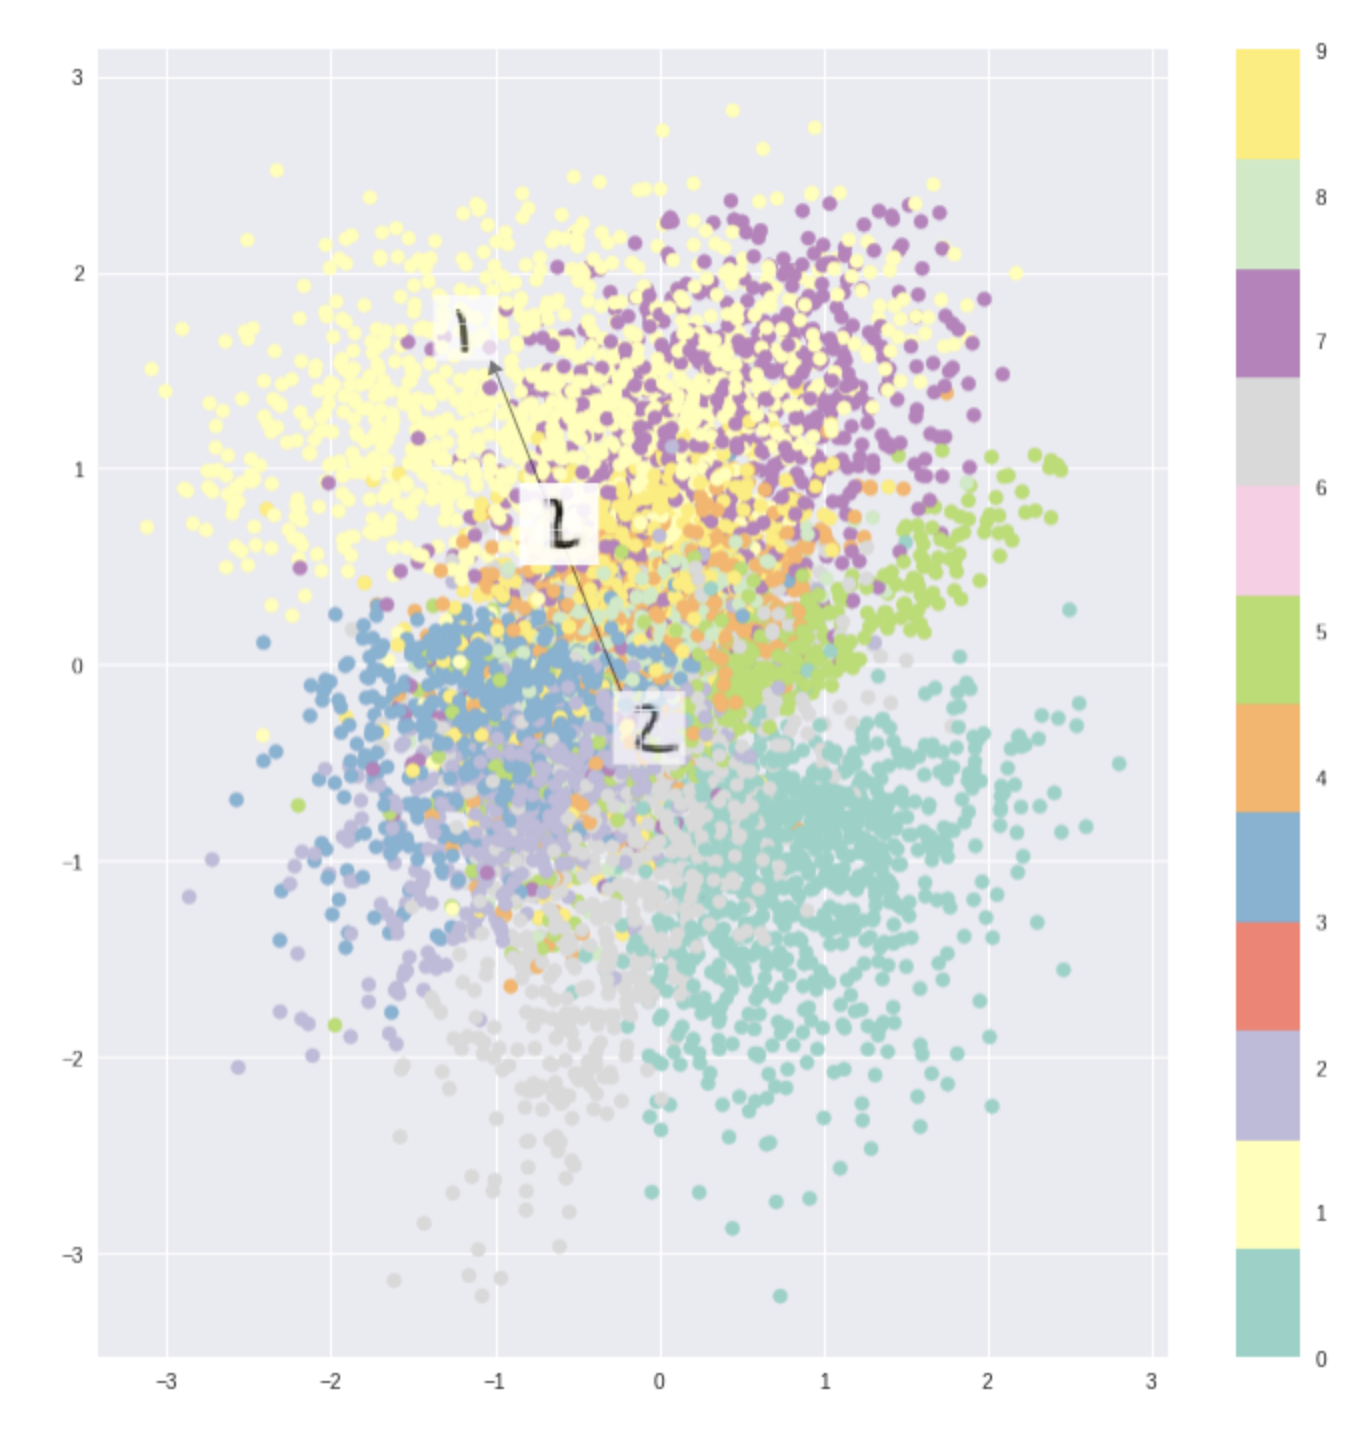
\includegraphics[width=2in]{pics/mnist-vae-c}
\end{figure}

  {\tiny Image credit: I.~Shafkat}
\end{frame}

\end{document}





%%% Local Variables:
%%% mode: latex
%%% TeX-master: t
%%% End:
